%%%% main.tex, 2022/08/10, 2.5
%%%% Copyright (C) 2020 Vinicius Pegorini (vinicius@utfpr.edu.br)
%%
%% This work may be distributed and/or modified under the conditions of the
%% LaTeX Project Public License, either version 1.3 of this license or (at your
%% option) any later version.
%% The latest version of this license is in
%%   http://www.latex-project.org/lppl.txt
%% and version 1.3 or later is part of all distributions of LaTeX version
%% 2005/12/01 or later.
%%
%% This work has the LPPL maintenance status `maintained'.
%%
%% The Current Maintainer of this work is Vinicius Pegorini.
%%
%% This work consists of the files utfprpb.cls, utfprpb.tex, and
%% utfprpb-dados.tex.
%%
%% The Current Maintainer of this work is Vinicius Pegorini.
%% Updated by:
%% - Marco Aurélio Graciotto Silva;
%% - Rogério Aparecido Gonçalves;
%% - Luiz Arthur Feitosa dos Santos.
%%
%% This work consists of the files utfpr.cls, main.tex, and
%% variaveis.tex.
%% A brief description of this work is in readme.md.

%% ####################################################
%%
%% >> Atenção - Leia isso antes de usar esse template<< 
%%
%% Esse template foi desenvolvido por professores,  com a intenção de ajudar os alunos com as entregas na biblioteca. Não há uma equipe especializada e dedicada mantendo tal template, mas sim professores trabalhando além das suas funções básicas, que são: ensino, pesquisa e extensão.
%
%% Também os mantenedores deste template não são especializados em LaTeX, muito menos em normas da ABNT. Todos que contribuíram com o template fizeram isso visando deixá-lo o mais próximo possível das normas da ABNT e das regras, anseios e expectativas da biblioteca da UTFPR. É muito importante entender que os desenvolvedores do template não têm relação direta com a biblioteca ou com a ABNT. Ou seja, não são os desenvolvedores do template que ditam as regras e normas dos textos que devem ser entregues à biblioteca.

%%É válido informar também, que como não há uma equipe dedicada e especializada, o tempo para colaborar com o template é curto. Desta forma, pode ser que não sejam empregadas as melhores técnicas, métodos e ferramentas para o desenvolvimento do template. Também pode acontecer do template não atender completamente todos os anseios e exigências da ABNT e da biblioteca, pois por exemplo, muitas regras de redação possuem questões interpretativas. Assim, o template sempre estará em contínua evolução e seria extremamente interessante que as pessoas (alunos,  professores,  técnicos e entusiastas) colaborarem com a evolução do template. Toda ajuda será bem vinda! Isso pode ser feito enviando e-mail para os desenvolvedores, desta forma, assim que possível esses vão tentar melhorar o template.

%%O template é apenas mais uma ferramenta para o desenvolvimento de trabalhos para a biblioteca. Todavia, podem existir outros templates LaTeX. Assim como há templates em outros formatos, que não o LaTeX. O mais importante é que qualquer pessoa, utilizando a princípio qualquer ferramenta, pode desenvolver textos que atendem os requisitos da biblioteca apenas estudando, interpretando e seguindo as regras da UTFPR e da ABNT, que estão disponíveis na página Web da instituição. O template é só um facilitador.

%%Por fim,  é necessário entender que infelizmente o ambiente LaTeX pode ser complexo e gerar resultados distintos dependendo do: sistema operacional,  pacotes LaTeX utilizados,  configurações alteradas, editor utilizado, a forma que está sendo redigida textos, figuras,  etc. Assim não há como garantir que o resultado final será o esperado.  Dito tudo isso,  >>UTILIZE ESSE TEMPLATE POR SUA CONTA E RISCO<<. Os desenvolvedores e colaboradores deste template não se responsabilizam pelo resultado do uso deste template e se eximem de qualquer responsabilidade.

%###################################################


% Luiz - pdfa: inclusão do pdfa
\PassOptionsToPackage{
	pdfa
}{hyperref}



%% Classe e opções de documento
\documentclass[%% Opções
%% -- Opções da classe memoir --
  12pt,%% Tamanho da fonte: 10pt, 11pt, 12pt, etc.
  a4paper,%% Tamanho do papel: a4paper (A4), letterpaper (carta), etc.
  % fleqn,%% Alinhamento das equações à esquerda (comente para alinhamento centralizado)
  % leqno,%% Numeração das equações no lado esquerdo (comente para lado direito)
  oneside,%% Impressão dos elementos textuais e pós-textuais: oneside (anverso) ou twoside (anverso e verso, se mais de 100 p.)
  openright,%% Impressão da primeira página dos capítulos: openright (anverso), openleft (verso) ou openany (anverso e verso)
%% -- Opções da classe abntex2 --
  sumario = abnt-6027-2012,%% Formatação do sumário: tradicional (estilo tradicional) ou abnt-6027-2012 (norma ABNT 6027-2012)
  chapter = TITLE,%% Títulos de capítulos em maiúsculas (comente para desabilitar)
  % luiz - comentar section para ser minusculo
  %section = TITLE,%% Títulos de seções secundárias em maiúsculas (comente para desabilitar)
  % subsection = TITLE,%% Títulos de seções terciárias em maiúsculas (comente para desabilitar)
  % subsubsection = TITLE,%% Títulos de seções quartenárias em maiúsculas (comente para desabilitar),
%% -- Opções da classe utfprpgtex --
  pretextualoneside,%% Impressão dos elementos pré  -textuais: pretextualoneside (anverso) ou pretextualtwoside (anverso e verso)
  fontetimes,%% Fonte do texto: fontetimes (times), fontearial (arial) ou fontecourier (courier)
  % vinculoscoloridos,%% Cores nos vínculos (citações, arquivos, links, url, etc.) (comente para desabilitar)
  semrecuonosumario,%% Remoção do recuo dos itens no sumário (comente para adição do recuo, se estilo tradicional)
  usemakeindex,%% Compilação de glossários e índices utilizando makeindex (comente para desabilitar)
  % legendascentralizadas,%% Alinhamento das legendas centralizado (comente para alinhamento à esquerda)
  %aprovacaoestiloppg,%% Folha de aprovação do programa de pós-graduação no estilo do PPG (comente para estilo padrão)
  pardeassinaturas,%% Assinaturas na folha de aprovação em até duas colunas (comente para em uma única coluna)
  % linhasdeassinaturas,%% Linhas de assinaturas na folha de aprovação (comente para remover as linhas)
%% -- Opções do pacote babel --
  english,%% Idioma adicional para hifenização
  french,%% Idioma adicional para hifenização
  spanish,%% Idioma adicional para hifenização
  brazil,%% Idioma principal do documento (último da lista)
]{utfpr}%% Classe utfpr

% Luiz: pdfa: necessário para criar pdfa
\usepackage[a-3b,mathxmp]{pdfx}[2018/12/22] % você pode escolher entre a-1b, a-2b, a-3b - o template ainda não suporta o a-Xa de 

\usepackage{float}

%%%% configuracoes.tex, 2022/05/02, 2.4a

%% ####################################################
%%
%% >> Atenção - Leia isso antes de usar esse template<< 
%%
%% Esse template foi desenvolvido por professores,  com a intenção de ajudar os alunos com as entregas na biblioteca. Não há uma equipe especializada e dedicada mantendo tal template, mas sim professores trabalhando além das suas funções básicas, que são: ensino, pesquisa e extensão.
%
%% Também os mantenedores deste template não são especializados em LaTeX, muito menos em normas da ABNT. Todos que contribuíram com o template fizeram isso visando deixá-lo o mais próximo possível das normas da ABNT e das regras, anseios e expectativas da biblioteca da UTFPR. É muito importante entender que os desenvolvedores do template não têm relação direta com a biblioteca ou com a ABNT. Ou seja, não são os desenvolvedores do template que ditam as regras e normas dos textos que devem ser entregues à biblioteca.

%%É válido informar também, que como não há uma equipe dedicada e especializada, o tempo para colaborar com o template é curto. Desta forma, pode ser que não sejam empregadas as melhores técnicas, métodos e ferramentas para o desenvolvimento do template. Também pode acontecer do template não atender completamente todos os anseios e exigências da ABNT e da biblioteca, pois por exemplo, muitas regras de redação possuem questões interpretativas. Assim, o template sempre estará em contínua evolução e seria extremamente interessante que as pessoas (alunos,  professores,  técnicos e entusiastas) colaborarem com a evolução do template. Toda ajuda será bem vinda! Isso pode ser feito enviando e-mail para os desenvolvedores, desta forma, assim que possível esses vão tentar melhorar o template.

%%O template é apenas mais uma ferramenta para o desenvolvimento de trabalhos para a biblioteca. Todavia, podem existir outros templates LaTeX. Assim como há templates em outros formatos, que não o LaTeX. O mais importante é que qualquer pessoa, utilizando a princípio qualquer ferramenta, pode desenvolver textos que atendem os requisitos da biblioteca apenas estudando, interpretando e seguindo as regras da UTFPR e da ABNT, que estão disponíveis na página Web da instituição. O template é só um facilitador.

%%Por fim,  é necessário entender que infelizmente o ambiente LaTeX pode ser complexo e gerar resultados distintos dependendo do: sistema operacional,  pacotes LaTeX utilizados,  configurações alteradas, editor utilizado, a forma que está sendo redigida textos, figuras,  etc. Assim não há como garantir que o resultado final será o esperado.  Dito tudo isso,  >>UTILIZE ESSE TEMPLATE POR SUA CONTA E RISCO<<. Os desenvolvedores e colaboradores deste template não se responsabilizam pelo resultado do uso deste template e se eximem de qualquer responsabilidade.

%###################################################

%% Pacotes carregados nas classes:
%%   memoir: abstract, appendix, array, booktabs, ccaption, chngcntr, chngpage, dcolumn, delarray, enumerate, epigraph, framed,
%%           ifmtarg, ifpdf, index, makeidx, moreverb, needspace, newfile, nextpage, parskip, patchcmd, setspace, shortvrb, showidx,
%%           tabularx, titleref, titling, tocbibind, tocloft, verbatim, verse.
%%   memoir (similares): crop, fancyhdr, geometry, sidecap, subfigure, titlesec.
%%   abntex2: babel, bookmark, calc, enumitem, ifthen, hyperref, textcase.
%%   utfprpgtex: abntex2cite, ae, algorithmic, amsmath, backref, breakurl, caption, cmap, color, eepic, epic, epsfig, etoolbox,
%%               fancyhdr, fix-cm, fontenc, glossaries, graphics, graphicx, helvet, hyphenat, indentfirst, inputenc, lastpage,
%%               morewrites, nomencl, sfmath, sistyle, substr, times, xtab.


%% Pacotes adicionais (\usepackage[options]{package})
\usepackage{bigdelim, booktabs, colortbl, longtable, multirow}%% Ferramentas para tabelas
\usepackage{amssymb, amstext, amsthm, icomma}%% Ferramentas para linguagem matemática
\usepackage{pifont, textcomp, wasysym}%% Símbolos de texto
\usepackage{lipsum}				% para geração de dummy text
\usepackage{subfig}             % para adicionar figuras lado a lado no texto                    
\usepackage{pdfpages}           % para adicionar documentos pdf ao trabalho
\usepackage{xspace}


% luiz: primeira letra maiúscula
% solução 1
%\usepackage{stringstrings}
%\newcommand{\firstcap}[1]{\caselower[e]{#1}\capitalize{\thestring}}

% solução 2 - não usei essa
% \usepackage[utf8]{inputenc}
% \usepackage{datatool-base}
% \usepackage{mfirstuc}

% Formatação do título da seção - primeira letra caixa alta e o resto em caixa baixa.
% \usepackage[explicit]{titlesec}
% \usepackage{lipsum}
% \titleformat{\section}{\normalfont}{\thesection}{1em}{\textbf{\firstcap{#1}}} % funciona mas apenas para o título da seção e não para o sumário (a configuração do sumário está mais para baixo

% luiz: define o underline colorido.
% https://github.com/abntex/abntex2-contrib/blob/master/customizacoes/pucminas/abntex2-pucminas.sty
% acabei não usando o black e o coloruline da solução do link

\usepackage[normalem]{ulem} % para o underline colorido na seção quaternária
\renewcommand*{\cftsubsubsectionfont}{\normalfont\uline} % underline no sumário
\setsubsubsecheadstyle{\ABNTEXsubsubsectionfont\ABNTEXsubsubsectionfontsize\ABNTEXsubsubsectionupperifneeded\uline} %underline no título da subsubsection

% luiz: bibliografia - opções

%% Comandos personalizados (\newcommand{name}[num]{definition})
\newcommand{\cpp}{\texttt{C$++$}}%% C++
\newcommand{\latex}{\LaTeX\xspace}%% LaTeX
\newcommand{\ds}{\displaystyle}%% Tamanho normal das equações
\newcommand{\bsym}[1]{\boldsymbol{#1}}%% Texto no modo matemático em negrito
\newcommand{\mr}[1]{\mathrm{#1}}%% Texto no modo matemático normal (não itálico)
\newcommand{\der}{\mr{d}}%% Operador diferencial
\newcommand{\deri}[2]{\frac{\der #1}{\der #2}}%% Derivada ordinária
\newcommand{\derip}[2]{\frac{\partial #1}{\partial #2}}%% Derivada parcial
\newcommand{\pare}[1]{\left( #1 \right)}%% Parênteses
\newcommand{\colc}[1]{\left[ #1 \right]}%% Colchetes
\newcommand{\chav}[1]{\left\lbrace #1 \right\rbrace}%% Chaves
\newcommand{\sen}{\operatorname{sen}}%% Operador seno
\newcommand{\senh}{\operatorname{senh}}%% Operador seno hiperbólico
\newcommand{\tg}{\operatorname{tg}}%% Operador tangente
\newcommand{\tgh}{\operatorname{tgh}}%% Operador tangente hiperbólico
\newcommand{\seqref}[1]{Equação~\eqref{#1}}%% Referência de uma única equação
\newcommand{\meqref}[1]{Equações~\eqref{#1}}%% Referência de múltiplas equações
\newcommand{\citep}[1]{\cite{#1}}%% Atalho para citação implícita
\newcommand{\citet}[1]{\citeonline{#1}}%% Atalho para citação explícita
\newcommand{\citepa}[1]{(\citeauthor{#1})}%% Atalho para citação implícita (somente autor)
\newcommand{\citeta}[1]{\citeauthoronline{#1}}%% Atalho para citação explícita (somente autor)
\newcommand{\citepy}[1]{(\citeyear{#1})}%% Atalho para citação implícita (somente ano)
\newcommand{\citety}[1]{\citeyear{#1}}%% Atalho para citação explícita (somente ano)

\newcommand{\fonteTexto}[1]{\renewcommand{\familydefault}{#1}}

% Define o caminho das figuras
\graphicspath{{figuras/}}

% Define a fonte ara helvet que é uma fonte similar à Arial, se for usar a Arial tem que mudar o compilador para XeLaTex, mas ai tem que arrumar os erros: https://latex.org/forum/viewtopic.php?t=25998
%\usepackage{helvet}
%\renewcommand{\familydefault}{\sfdefault}
%\usepackage{times} % para fonte time new roman
%\usepackage{pslatex} % ou essa aqui...

%\usepackage{titlesec}

%% Configuração de glossário
% \usepackage[portuguese]{nomencl}
% \usepackage[nogroupskip,nonumberlist,nopostdot,nohypertypes={acronym}]{glossaries}
% \makenoidxglossaries
\usepackage{glossaries}
\makeglossaries

% para siglas em português
\newcommand{\siglaPt}[2]
{
 \newglossaryentry{#1}{
  name=#1,
  description={#2},
  first={#2 (#1)},
  long={#2}
 }  
}

% para siglas de língua estrangeira, nessas a descrição longa fica em itálico.
\newcommand{\siglaIt}[2]
{
 \newglossaryentry{#1}{
  name=#1,
  description={\textit{#2}},
  first={\textit{#2} ({#1})},
  long={\textit{#2}}
 }  
}

%% luiz - para fazer os avisos
\usepackage{tcolorbox}

% use para criar caixas de avisos, pode ser utilizado para fazer anotações de tarefas indicadas pelo orientador/banca.
% \caixa{Atenção}{texto...}
\newcommand{\caixa}[2]{
\begin{tcolorbox}[colback=red!5!white,colframe=red!45!white, title = #1, fonttitle=\bfseries]
#2
\end{tcolorbox}
}

% Luiz - Linhas órfãs e viúvas
\widowpenalty=10000
\clubpenalty=10000

% Luiz - Caption do tamanho da Tabela
%\usepackage[width=1\textwidth]{caption}

% Luiz - configurar a margem dos itens
\setlength{\leftmargini}{1.5cm}
\setlength{\leftmarginii}{1.5cm}

\usepackage[utf8]{inputenc} %Pacote para acentuação
%\usepackage[portuguese,brazilian]{babel}

%% Arquivo de dados do modelo de documento LaTeX para produção de trabalhos acadêmicos da UTFPR
%%%% variaveis.tex, 2022/05/02, 2.4a
%%%% Copyright (C) 2020 Vinicius Pegorini (vinicius@utfpr.edu.br)
%%
%% This work may be distributed and/or modified under the conditions of the
%% LaTeX Project Public License, either version 1.3 of this license or (at your
%% option) any later version.
%% The latest version of this license is in
%%   http://www.latex-project.org/lppl.txt
%% and version 1.3 or later is part of all distributions of LaTeX version
%% 2005/12/01 or later.
%%
%% This work has the LPPL maintenance status `maintained'.
%%
%% The Current Maintainer of this work is Vinicius Pegorini.
%% Updated by:
%% - Marco Aurélio Graciotto Silva;
%% - Rogério Aparecido Gonçalves;
%% - Luiz Arthur Feitosa dos Santos.
%%
%% This work consists of the files utfpr.cls, main.tex, and
%% variaveis.tex.
%%
%% A brief description of this work is in readme.txt.

%% ####################################################
%%
%% >> Atenção - Leia isso antes de usar esse template<< 
%%
%% Esse template foi desenvolvido por professores,  com a intenção de ajudar os alunos com as entregas na biblioteca. Não há uma equipe especializada e dedicada mantendo tal template, mas sim professores trabalhando além das suas funções básicas, que são: ensino, pesquisa e extensão.
%
%% Também os mantenedores deste template não são especializados em LaTeX, muito menos em normas da ABNT. Todos que contribuíram com o template fizeram isso visando deixá-lo o mais próximo possível das normas da ABNT e das regras, anseios e expectativas da biblioteca da UTFPR. É muito importante entender que os desenvolvedores do template não têm relação direta com a biblioteca ou com a ABNT. Ou seja, não são os desenvolvedores do template que ditam as regras e normas dos textos que devem ser entregues à biblioteca.

%%É válido informar também, que como não há uma equipe dedicada e especializada, o tempo para colaborar com o template é curto. Desta forma, pode ser que não sejam empregadas as melhores técnicas, métodos e ferramentas para o desenvolvimento do template. Também pode acontecer do template não atender completamente todos os anseios e exigências da ABNT e da biblioteca, pois por exemplo, muitas regras de redação possuem questões interpretativas. Assim, o template sempre estará em contínua evolução e seria extremamente interessante que as pessoas (alunos,  professores,  técnicos e entusiastas) colaborarem com a evolução do template. Toda ajuda será bem vinda! Isso pode ser feito enviando e-mail para os desenvolvedores, desta forma, assim que possível esses vão tentar melhorar o template.

%%O template é apenas mais uma ferramenta para o desenvolvimento de trabalhos para a biblioteca. Todavia, podem existir outros templates LaTeX. Assim como há templates em outros formatos, que não o LaTeX. O mais importante é que qualquer pessoa, utilizando a princípio qualquer ferramenta, pode desenvolver textos que atendem os requisitos da biblioteca apenas estudando, interpretando e seguindo as regras da UTFPR e da ABNT, que estão disponíveis na página Web da instituição. O template é só um facilitador.

%%Por fim,  é necessário entender que infelizmente o ambiente LaTeX pode ser complexo e gerar resultados distintos dependendo do: sistema operacional,  pacotes LaTeX utilizados,  configurações alteradas, editor utilizado, a forma que está sendo redigida textos, figuras,  etc. Assim não há como garantir que o resultado final será o esperado.  Dito tudo isso,  >>UTILIZE ESSE TEMPLATE POR SUA CONTA E RISCO<<. Os desenvolvedores e colaboradores deste template não se responsabilizam pelo resultado do uso deste template e se eximem de qualquer responsabilidade.

%###################################################

%% Documento
%% Luiz: Define a fonte do texto da monografia
\fonteTexto{\sfdefault} % utilize \rmdefault para Times New Roman ou \sfdefault para Arial
\TipoDeDocumento{Trabalho de Conclusão de Curso de Graduação}%% Tipo de documento: "Tese", "Dissertação" ou "Trabalho de Conclusão de Curso de Graduação", "Estágio Supervisionado"
\NivelDeFormacao{Bacharelado}%% Nível de formação: "Doutorado", "Mestrado", "Bacharelado" ou "Tecnólogo" - ATENÇÃO, isso será utilizado para alterar a formatação do trabalho, pois pode haver formatações distintas dependendo o nível/tipo de trabalho.


%% luiz
% Template LaTex criado pelo Departamento Acadêmico de Computação (DACOM)
% da Universidade Tecnológica Federal do Paraná - Campus Campo Mourão (UTFPR-CM)
% Criado e alterado pelos professores:
% - Marco Aurélio Graciotto Silva
% - Rogério Aparecido Gonçalvez
% - Luiz Arthur Feitosa dos Santos
% Esse template utiliza a licença CC BY:
% Esta licença permite que outros distribuam, remixem, adaptem e criem a partir deste trabalho, mesmo para fins comerciais, desde que atribuam o devido crédito pela criação original.
% https://creativecommons.org/licenses/by/4.0/deed.pt_BR

% Dados do curso. Caso seja BCC:
\program{Curso de Bacharelado em Engenharia Eletrônica}
\programen{Undergradute Program in Electronic Engineering}
\degree{Bacharel}
\degreearea{Engenharia Eletrônica}
% Caso seja TSI:
% \program{Curso Superior de Tecnologia em Sistemas para Internet}
% \programen{Undergradute Program in Tecnology for Internet Systems}
% \degree{Tecnólogo}
% \degreearea{Tecnologia em Sistemas para Internet}


% Dados da disciplina. Escolha uma das opções e a descomente:
% TCC1:
%\goal{Proposta de Trabalho de Conclusão de Curso de Graduação}
%\course{Trabalho de Conclusão de Curso 1}
% TCC2:
 \goal{Trabalho de Conclusão de Curso de Graduação}
 \course{Trabalho de Conclusão de Curso 2}


% Dados do TCC (precisa alterar)
\author{Alessandro Massayuki Nakatani\\
        José Mário Nishihara de Albuquerque}  % Seu nome
\authorbib{Albuquerque, José Mário Nishihara de } % Seu nome para referência bibliográfica (Sobrenome, Nome)
\title{Análise do Uso de Informações de Profundidade para Classificação de Objetos em Sistemas Elétricos de Potência com um Sensor Multimodal 
} % Título do trabalho
\titleFA{}
\titleen{}
\advisor{Prof. Dr. Ronnier Frates Rohrich} % Nome do orientador. Lembre-se de prefixar com "Prof. Dr.", "Profª. Drª.", "Prof. Me." ou "Profª. Me."}
% Se não houver corientador, comente a linha a baixo
\coadvisor{Prof. Dr. André Schneider de Oliveira} % Nome do coorientador, caso exista. Caso não exista, comente a linha.
\depositshortdate{2025} % Ano em que depositou este documento
\approvaldate{dia / mês  / ano}

% Dados do curso que não precisam de alteração
\university{Universidade Tecnológica Federal do Paraná}
\universityen{Federal University of Technology -- Paraná}
\universitycampus{Campus Curitiba}
\universityunit{Departamento Acadêmico de Eletrônica}
\address{CURITIBA}
\addressen{Campus Curitiba, PR, Brazil}
\documenttype{Monografia}
\documenttypeen{Monograph}
\degreetype{Graduação}

\evalboardmember{Nome completo e por extenso do Membro 1 (de acordo com o Currículo Lattes)
}{Titulação (Especialização, Mestrado, Doutorado)}{Nome completo e por extenso da instituição a qual possui vínculo}
\evalboardmember{Nome completo e por extenso do Membro 2 (de acordo com o Currículo Lattes)
}{Titulação (Especialização, Mestrado, Doutorado)}{Nome completo e por extenso da instituição a qual possui vínculo}
\evalboardmember{Nome completo e por extenso do Membro 3 (de acordo com o Currículo Lattes)
}{Título (Titulação (Especialização, Mestrado, Doutorado)}{Nome completo e por extenso da instituição a qual possui vínculo}
%\evalboardmember{Nome completo e por extenso do Membro 4}{Título (especialização, mestrado, doutorado}{Nome completo e por extenso da instituição a qual possui vínculo}

%% Palavras-chave e keywords
%% ATENÇÃO - você deve indicar a quantidade de palavras chaves para o template LaTeX utilizar o pontuação correta!
\NumeroDePalavrasChave{5}%% Número de palavras-chave (máximo 5)
%% Atenção - por enquanto o template não está suportando acentos normais na palavra chave, por isso caso a palavra tenha acento, você deve utilizar o estilo antigo do LaTeX, sendo os acentos: á - \'a  é - \'e   â - \^a  ê - \^e  à - \`a  ä - \"a  ç - \c{c}
\PalavraChaveA{aprendizado de m\'aquina}%% Palavra-chave A
\PalavraChaveB{sensores de profundidade}%% Palavra-chave B
\PalavraChaveC{inspe\c{c}\~ao aut\^onoma}%% Palavra-chave C
\PalavraChaveD{classifica\c{c}\~ao de objetos}%% Palavra-chave D
\PalavraChaveE{linhas de transmiss\~ao}%% Palavra-chave E
%% Exemplo de como utilizar acentos na Palavra-chave:
% \PalavraChaveA{ol\'a}%% Olá
%\PalavraChaveB{voc\^e}%% você
%\PalavraChaveC{\`a}%% à
%\PalavraChaveD{a\c{c}\~ao}%% ação
%\PalavraChaveE{arg\"uir}%% argüir


%% ATENÇÃO - você deve indicar a quantidade de keywords para o template LaTeX utilizar o pontuação correta!
\NumeroDeKeywords{4}%% Número de keywords (máximo 5)
\KeywordA{machine learning}%% Keyword A
\KeywordB{deep sensors}%% Keyword B
\KeywordC{autonomous inspection}%% Keyword C
\KeywordD{power lines}%% Keyword D
%\KeywordE{Keyword 5}%% Keyword E


% É obrigatório o uso de uma licença Creative Commons (CC) nos trabalhos de TCC pelos cursos ligados a DACOM da UTFPR-CM.
% Veja: http://portal.utfpr.edu.br/biblioteca/trabalhos-academicos/docentes/procedimento-de-entrega-graduacao

% Sendo assim, escolha com o seu orientador uma das licenças CC a seguir: 

% CC BY: Esta licença permite que outros distribuam, remixem, adaptem e criem a partir deste trabalho, mesmo para fins comerciais, desde que atribuam o devido crédito pela criação original. Essa é a menos restritiva.
\licenca{ccbync}

% CC BY CA: Esta licença permite que outros remixem, adaptem e criem a partir deste trabalho, mesmo para fins comerciais, desde que atribuam o devido crédito e que licenciem as novas criações sob termos idênticos.
%\licenca{ccbysa}

% CC BY ND: Esta licença permite a redistribuição, comercial e não comercial, desde que o trabalho seja distribuído inalterado e no seu todo, com crédito ao autor.
%\licenca{ccbynd}

% CC BY NC: Esta licença permite que outros remixem, adaptem e criem a partir deste trabalho para fins não comerciais, e embora os novos trabalhos tenham de atribuir o devido crédito e não possam ser usados para fins comerciais, os trabalhos derivados não têm que serem licenciados sob os mesmos termos.
%\licenca{ccbync}

% CC BY NC SA: Esta licença permite que outros remixem, adaptem e criem a partir deste trabalho para fins não comerciais, desde que atribuam ao autor o devido crédito e que licenciem as novas criações sob termos idênticos.
%\licenca{ccbyncsa}

% CC BY NC ND: Esta licença só permite que outros façam download do trabalho e o compartilhe desde que atribuam crédito ao autor, mas sem que possam alterá-los de nenhuma forma ou utilizá-los para fins comerciais. Essa é a mais restritiva.
%\licenca{ccbyncnd}

% Deixar sem licença - isso é aplicado apenas aos trabalhos que não são obrigados a ter licença. Na duvida verifique isso com o seu orientador e professor responsável pelo TCC. Para deixar o texto sem licença deixe o comando licença em brando ou deixe comentado.
%\licenca{}
% by DACOM/UTFPR-CM%% Realize as modificações pertinentes no arquivo "utfprpb-dados.tex"

%% Ferramenta para criação de índices
\makeindex%% Não comente esta linha

%% Ferramenta para criação de glossários
\makeglossaries%% Não comente esta linha

%%%% LISTA DE ABREVIATURAS E SIGLAS 
%%
%% Relação, em ordem alfabética, das abreviaturas (representação de uma palavra por meio de alguma(s) de sua(s) sílaba(s) ou
%% letra(s)), siglas (conjunto de letras iniciais dos vocábulos e/ou números que representa um determinado nome) e acrônimos
%% (conjunto de letras iniciais dos vocábulos e/ou números que representa um determinado nome, formando uma palavra pronunciável).
%%
%% Este arquivo para definição de abreviaturas, siglas e acrônimos é utilizado com a opção "glossaries" (pacote)

%% Abreviaturas: \abreviatura{rótulo}{representação}{definição}

\abreviatura{art.}{art.}{Artigo}
\abreviatura{cap.}{cap.}{Capítulo}
\abreviatura{sec.}{sec.}{Seção}

%% Siglas: \sigla{rótulo}{representação}{definição}

\sigla{abnt}{ABNT}{Associação Brasileira de Normas Técnicas}
\sigla{cnpq}{CNPq}{Conselho Nacional de Desenvolvimento Científico e Tecnológico}
\sigla{eps}{EPS}{\textit{Encapsulated PostScript}}
\sigla{pdf}{PDF}{Formato de Documento Portátil, do inglês \textit{Portable Document Format}}
\sigla{ps}{PS}{\textit{PostScript}}
\sigla{utfpr}{UTFPR}{Universidade Tecnológica Federal do Paraná}


%% LEIA:

%% Para usar o \gls, você deve colocar a sigla aqui em \sigla

%% ADICIONAR SIGLAS: Quando você inclui alguma sigla, pode ser necessário compilar umas duas vezes para essa aparecer na lista de siglas.

%% ATENÇÃO REMOVER SIGLAS: se você remover a sigla do seu texto (não for usar mais), você deve comentar essa aqui e remover os \gls{} dessa sigla (se não vai ficar aparecendo a sigla na lista). Em caso de ERRO, quando o LaTeX informa que você ainda tem a sigla no texto, mesmo que não tenha. Você deve limpar o cache - no OverLeaf, clique no erro, vá:
%  ->view error
%%   ->(role para baixo, até o final)
%%     ->e clique em Clear cached files


%% Acrônimos: \acronimo{rótulo}{representação}{definição}
%\acronimo{gimp}{Gimp}{Programa de Manipulação de Imagem GNU, do inglês \textit{GNU Image Manipulation Program}}
%% Entradas da lista de abreviaturas e siglas - Comente para remover este item
%%%% GLOSSÁRIO
%%
%% Relação de palavras ou expressões técnicas de uso restrito ou de sentido obscuro, utilizadas no texto, acompanhadas das
%% respectivas definições.

%% Entradas do glossário: \newglossaryentry{rótulo}{informações da entrada}

\newglossaryentry{pai}{%% Informações da entrada
  name        = {pai},
  plural      = {pais},
  description = {um exemplo de entrada pai que possui subentradas (entradas filhas)}
}

\newglossaryentry{componente}{%% Informações da entrada
  name        = {componente},
  plural      = {componentes},
  parent      = {pai},
  description = {um exemplo de uma entrada componente, subentrada da entrada chamada \gls{pai}}
}

\newglossaryentry{filho}{%% Informações da entrada
  name        = {filho},
  plural      = {filhos},
  parent      = {pai},
  description = {um exemplo de uma entrada filha (subentrada) da entrada chamada \gls{pai}. Trata-se de uma entrada irmã da entrada chamada \gls{componente}}
}

\newglossaryentry{equilibrio}{%% Informações da entrada
  name        = {equilíbrio da configuração},
  see         = [veja também]{componente},
  description = {uma consistência entre os \glspl{componente}}
}

\newglossaryentry{tex}{%% Informações da entrada
  name        = {\TeX},
  sort        = {TeX},
  description = {é um sistema de tipografia criado por Donald E. Knuth}
}

\newglossaryentry{latex}{%% Informações da entrada
  name        = {\latex},
  sort        = {LaTeX},
  description = {um conjunto de macros para o processador de textos \gls{tex}, utilizado amplamente para a produção de textos matemáticos e científicos devido à sua alta qualidade tipográfica}
}

\newglossaryentry{bibtex}{%% Informações da entrada
  name        = {Bib\TeX},
  sort        = {BibTeX},
  parent      = {latex},
  description = {um software de gerenciamento de referências para a formatação de listas de referências. A ferramenta Bib\TeX\ é normalmente usada em conjunto com o sistema de preparação de documentos do \gls{latex}}
}

\newglossaryentry{abntex2}{%% Informações da entrada
  name        = {\abnTeX},
  sort        = {abnTeX2},
  see         = {latex},
  description = {uma suíte para \gls{latex} que atende os requisitos das normas da Associação Brasileira de Normas Técnicas (ABNT) para elaboração de documentos técnicos e científicos brasileiros, como artigos científicos, relatórios técnicos, trabalhos acadêmicos como teses, dissertações, projetos de pesquisa e outros documentos do gênero}
}

\newglossaryentry{utfprpbtex}{%% Informações da entrada
  name        = {\utfprpbtex},
  sort        = {UTFPRPBTeX},
  see         = {latex},
  parent      = {abntex2},
  description = {uma suíte para \gls{latex}, baseada na suíte \gls{abntex2}, que atende os requisitos das normas definidas pela Universidade Tecnológica Federal do Paraná (UTFPR), Câmpus Pato Branco, para elaboração de trabalhos acadêmicos}
}
%% Entradas do glossário - Comente para remover este item

%% Ferramenta para criação de nomenclaturas
\makenomenclature%% Não comente esta linha

%% Início do documento
\begin{document}%% Não comente esta linha



%% Formatação de páginas de elementos pré-textuais
\pretextual%% Não comente esta linha

%% Capa
%\incluircapa%% Comente para remover este item
\coverpageone

%% Folha de rosto (* coloca a ficha bibliográfica no verso)
%\incluirfolhaderosto*%% Comente para remover este item
\coverpagetwo

% luiz - iniciar contagem depois da folha de rosto
\clearpage
\setcounter{page}{2}

%% Ficha catalográfica (teses e dissertações)
%\incluirfichacatalografica%% Comente para remover este item

%% Errata
%%%%% ERRATA
%%
%% Lista dos erros ocorridos no texto, seguidos das devidas correções.

\begin{errata}%% Ambiente errata
\begin{table*}[htb]%% Ambiente table
\begin{tabularx}{\textwidth}{|l|l|X|X|}%% Ambiente tabularx
\hline
\textbf{Página(s)}         & \textbf{Linha(s)} & \textbf{Onde se lê} & \textbf{Leia-se}         \\ \hline
\pageref*{errata:capitulo} & 4, 9-11, 14-16    & capítulo(s)         & seção(ões) primária(s)   \\ \hline
\pageref*{errata:secao}    & 12-16             & seção(ões)          & seção(ões) secundária(s) \\ \hline
\pageref*{errata:subsecao} & 16                & subseção(ões)       & seção(ões) terciária(s)  \\ \hline
\end{tabularx}
\end{table*}
\end{errata}
%% Comente para remover este item

%% Folha de aprovação
%\incluirfolhaaprovacao
\approvalpage
%\incluirfolhadeaprovacao%% Para adicionar no formato de texto
%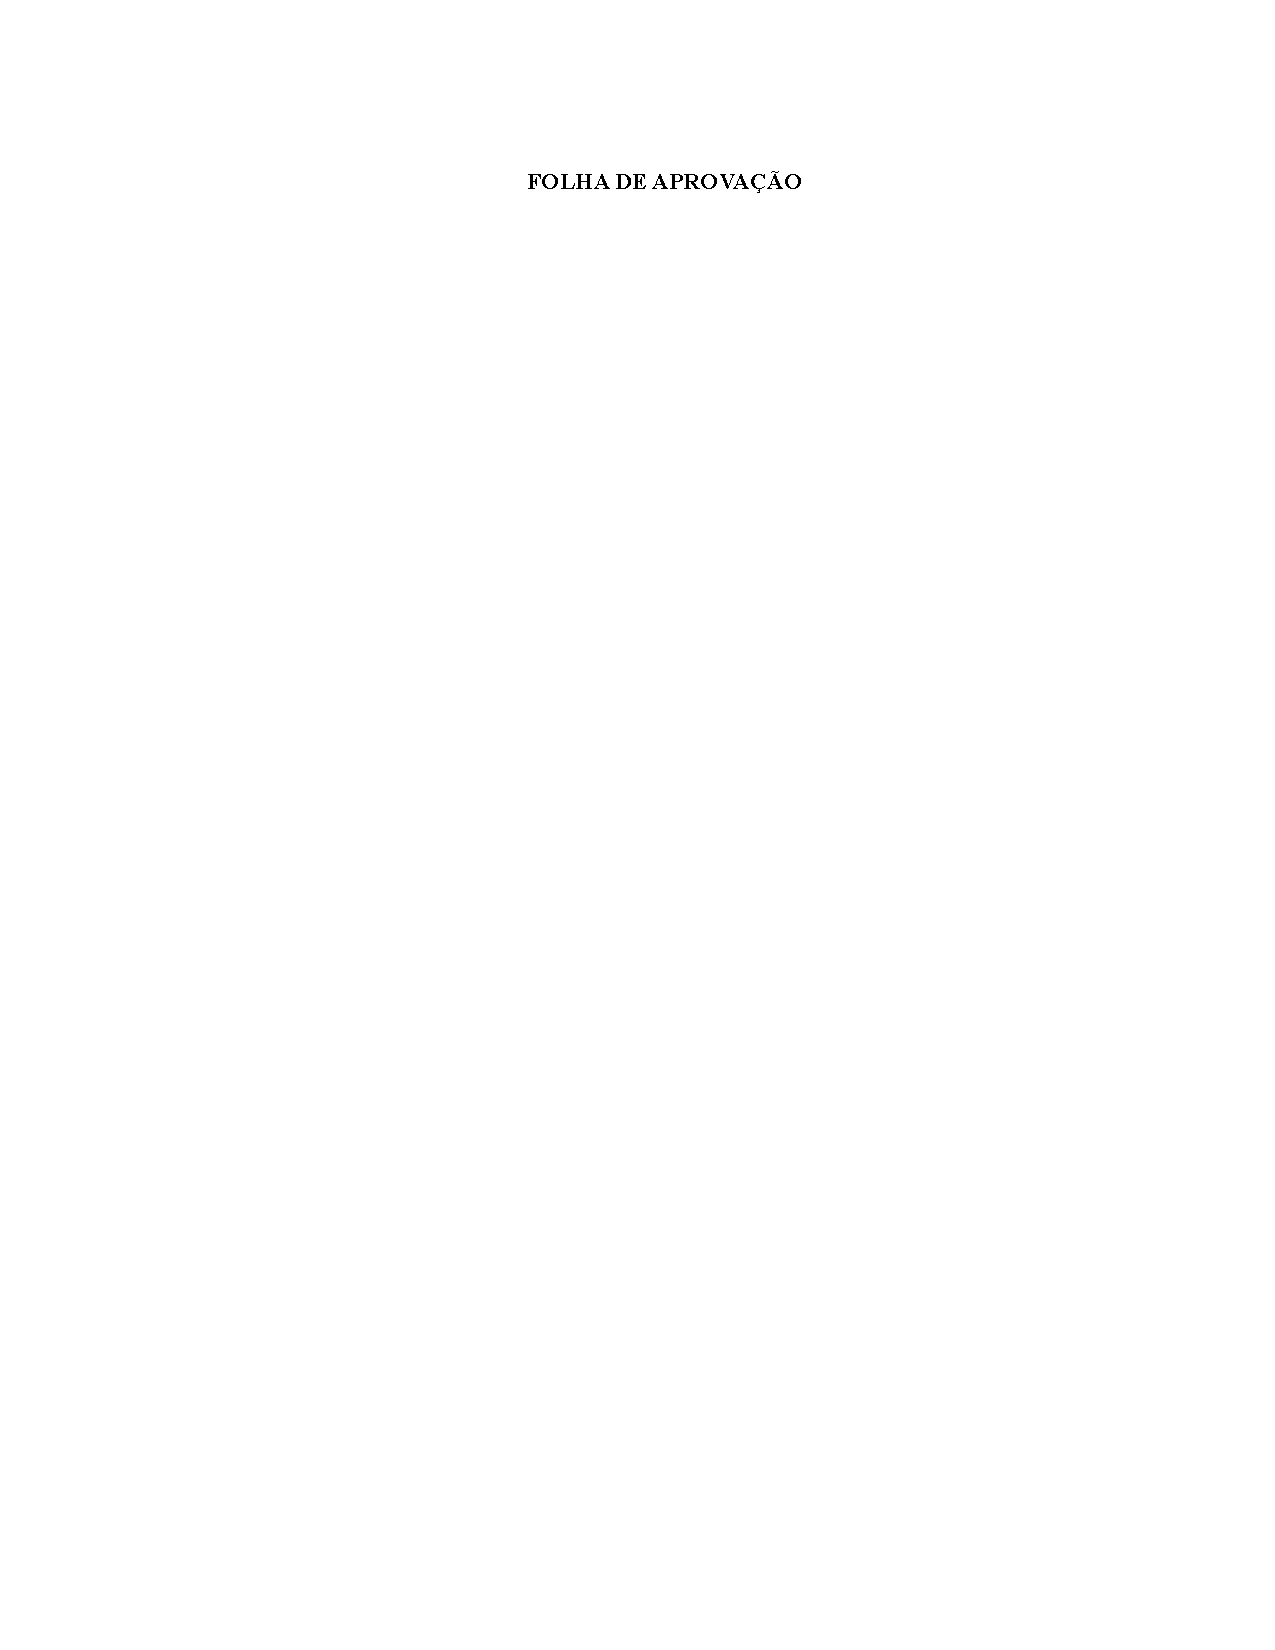
\includepdf[scale=1.0,pages=1]{./PreTexto/folha-aprovacao.pdf} % para adicionar o pdf enviado pelo professor apenas substitua o documento folha-aprovacao.pdf dentro da pasta PreTexto

%% Dedicatória
%%%% DEDICATÓRIA
%%
%% Texto em que o autor presta homenagem ou dedica seu trabalho.

\begin{dedicatoria}%% Ambiente dedicatoria

%Espaço destinado à dedicatória (elemento opcional). Folha que contém o oferecimento do trabalho à determinada pessoa ou pessoas. Exemplo:



Dedico este trabalho à minha família, pelos momentos de ausência.

\end{dedicatoria}
%% Comente para remover este item

%% Agradecimentos
%%%% AGRADECIMENTOS
%%
%% Texto em que o autor faz agradecimentos dirigidos àqueles que contribuíram de maneira relevante à elaboração do trabalho.

\begin{agradecimentos}%% Ambiente agradecimentos

Certamente estes parágrafos não irão atender a todas as pessoas que fizeram parte dessa importante fase de minha vida. Portanto, desde já peço desculpas àquelas que não estão presentes entre essas palavras, mas elas podem estar certas que fazem parte do meu pensamento e de minha gratidão. 

Agradeço ao(a) meu(minha) orientador(a) Prof.(a) Dr.(a) Nome Completo, pela sabedoria com que me guiou nesta trajetória.

Aos meus colegas de sala.

A Secretaria do Curso, pela cooperação.

Gostaria de deixar registrado também, o meu reconhecimento à minha família, pois acredito que sem o apoio deles seria muito difícil vencer esse desafio. 

Enfim, a todos os que por algum motivo contribuíram para a realização desta pesquisa.

%Espaço destinado aos agradecimentos (elemento opcional). Folha que contém manifestação de reconhecimento a pessoas e/ou instituições que realmente contribuíram com o(a) autor(a), devendo ser expressos de maneira simples. Exemplo:

%Não devem ser incluídas informações que nominem empresas ou instituições não nominadas no trabalho.

%Se o aluno recebeu bolsa de fomento à pesquisa, informar o nome completo da agência de fomento. Ex: Capes, CNPq, Fundação Araucária, UTFPR, etc. Incluir o número do projeto após a agência de fomento. Este item deve ser o último.

%Atenção: não utilizar este exemplo na versão final. Use a sua criatividade!


\end{agradecimentos}
%% Comente para remover este item

%% Epígrafe
%%%% EPÍGRAFE
%%
%% Texto em que o autor apresenta uma citação, seguida de indicação de autoria, relacionada com a matéria tratada no corpo do
%% trabalho.

\begin{epigrafe}%% Ambiente epigrafe
%
%Espaço destinado à epígrafe (elemento opcional). Nesta folha, o(a) autor(a) usa uma citação, seguida de indicação de autoria e ano, relacionada, preferencialmente, com o assunto tratado no corpo do trabalho. A citação deverá constar na lista de referências. Exemplo: 
%


\end{epigrafe}
%% Comente para remover este item

%% Resumo
%%%% RESUMO
%%
%% Apresentação concisa dos pontos relevantes de um texto, fornecendo uma visão rápida e clara do conteúdo e das conclusões do
%% trabalho.

\begin{resumoutfpr}%% Ambiente resumoutfpr

Este trabalho apresenta o desenvolvimento e avaliação de modelos de aprendizado de máquina aplicados à classificação de objetos em linhas de transmissão, utilizando dados de profundidade capturados por uma câmera \textit{RealSense D415}, um sensor LiDAR \textit{RPLIDAR A1} da Slamtec e a combinação de ambos. Foram testados cinco modelos - \textit{k-Nearest Neighbors}, Árvore de Decisões, \textit{Naive Bayes}, Rede Neural e Floresta Aleatória - com dados simulados e reais. Os resultados indicaram que o uso de apenas um dos sensores já permite uma classificação satisfatória, mas a fusão sensorial torna o sistema mais robusto. Os modelos mais leves apresentaram desempenho competitivo, evidenciando seu potencial para futura implementação embarcada. O estudo também explora técnicas de pré-processamento de imagens e dados para a criação de \textit{features} utilizadas no treinamento dos modelos. Destaca-se, assim, a viabilidade do uso de sensores de profundidade na inspeção autônoma de linhas de transmissão, com ganhos em segurança e redução de custos operacionais.

\end{resumoutfpr}
%De acordo com a NBR 6028:2021, a apresentação gráfica deve seguir o padrão do documento no qual o resumo está inserido. Para definição das palavras-chave (e suas correspondentes em inglês no abstract) consultar em Termo tópico do Catálogo de Autoridades da Biblioteca Nacional, disponível em: http://acervo.bn.gov.br/sophia_web/autoridade%% Comente para remover este item

%% Abstract
%%%% ABSTRACT
%%
%% Versão do resumo para idioma de divulgação internacional.

\begin{abstractutfpr}%% Ambiente abstractutfpr
Seguir o mesmo padrão do resumo, com a tradução do texto do resumo e referência, se houver, para a língua estrangeira (língua inglesa).
\end{abstractutfpr}
%% Comente para remover este item

%% Lista de algoritmos
%\incluirlistadealgoritmos%% Comente para remover este item


%% Lista de Ilustrações
%% Figuras, Gráficos, Quadros e Fotografias são incluídos juntos em uma mesma lista
%% Na UTFPR sugere-se adotar listas próprias, conforme a natureza da ilustração, a partir da existência de 3 elementos da mesma natureza.Neste caso, cada lista deverá iniciar em folha distinta. Não criar listas com apenas um item.


%\incluirlistadeilustracoes


%% Lista de figuras
\incluirlistadefiguras%% Comente para remover este item

%\incluirlistageraldeilustracoes
%\listofgeneralilust



%% Lista de Fotografias
%\incluirlistadefotografias %% Comente para remover este item


%% Lista de Gráficos
%\incluirlistadegraficos %% Comente para remover este item

%% Lista de tabelas
\incluirlistadetabelas%% Comente para remover este item

%% Lista de quadros
%\incluirlistadequadros

%% Listagem de códigos fonte
%\incluirlistadecodigosfonte

%% Lista de abreviaturas, siglas e acrônimos
\incluirlistadeacronimos{none}%% Opções: "glossaries" (pacote) ou "file" (arquivo) ou "none" (desabilita)

%% Lista de símbolos
\incluirlistadesimbolos{none}%% Opções: "nomencl" (pacote) ou "file" (arquivo) ou "none" (desabilita)

%% Sumário
\incluirsumario%% Comente para remover este item

%% Formatação de páginas de elementos textuais
\textual%% Não comente esta linha

%% Parte
% \part{Introdução}%% Comente para remover este item

%% Capítulo introdução - obrigatório
%------------------------------------------------------------%

\chapter{Introdução}
\label{cap:trabalhos:introducao}

\section{Inspeções e Classificação de Objetos em Linhas de Transmissão}

As inspeções periódicas em linhas de transmissão de alta tensão, pertencentes ao Sistema Elétrico de Potência (SEP), são essenciais para a manutenção da confiabilidade e segurança de todo o sistema, evitando acidentes e interrupções no fornecimento de energia elétrica. Essas estruturas operam em ambientes adversos e estão sujeitas a danos causados por condições climáticas extremas e objetos estranhos na fiação. \par
Existem diferentes métodos com finalidades específicas para a realização da inspeção, seja de modo preventivo ou corretivo. Tradicionalmente, o serviço é executado por equipes que escalam torres ou utilizam drones. Embora drones cubram grandes áreas com agilidade e baixo custo, enfrentam limitações como autonomia reduzida, dependência de visibilidade e menor precisão em detalhes complexos. Já a inspeção manual, apesar de precisa, apresenta altos custos, riscos operacionais, riscos de vida e baixa escalabilidade. \par
Com o avanço das tecnologias de inspeção, os métodos tradicionais aplicados em instalações de energia têm se mostrado insuficientes para atender às demandas atuais do setor, principalmente devido à baixa eficiência das inspeções manuais, aos altos riscos envolvidos e à detecção limitada de falhas potenciais. Nesse cenário, observa-se um crescente interesse na automação dessas tarefas por meio de sistemas robóticos embarcados, capazes de percorrer fisicamente os cabos das linhas de transmissão e realizar inspeções de forma autônoma e contínua. Tais sistemas podem ser equipados com sensores capazes de capturar informações detalhadas dos componentes da linha, mesmo em condições adversas. Entre os sensores, destacam-se as câmeras de profundidade, como a RealSense D415, e os sensores LiDAR, como o RPLIDAR A1, que permitem a obtenção de dados tridimensionais da cena com alta precisão. \par
Este trabalho investiga o uso de modelos de aprendizado de máquina para a classificação de objetos em linhas de transmissão, com dados de sensores em ambientes simulados e reais. A análise considera dados da RealSense, do LiDAR e a combinação dos dois, com foco na eficiência, no processamento embarcado e em técnicas de pré-processamento e extração de \textit{features}. Os objetos de interesse foram alguns dos mais populares presentes nas linhas: sinalizadores, amortecedores e isoladores.

\section{Justificativa}

Para que robôs autônomos de inspeção possam realizar rotinas de superação de obstáculos, existe a necessidade de classificação dos objetos presentes em linhas de transmissão. A identificação assertiva possibilita que o sistema opere de forma mais adequada àquela situação, uma vez que cada objeto possui diferentes dimensões, pontos de fixação e funcionalidades. Este trabalho consiste na interpretação de dados recebidos pelos sensores e seus respectivos tratamentos via modelos de aprendizado de máquina, buscando comparações de resultados e desempenho.

\section{Objetivos}
\subsection{Objetivos Gerais}

Avaliar o uso de sensores LiDAR 360º e RealSense para classificação de objetos em linhas de transmissão e avaliar os resultados com base no desempenho medido por métricas como acurácia, tempo de processamento e quantidade de informações utilizadas.

\subsection{Objetivos Específicos}

Desenvolvimento de Códigos de Configuração e Acionamento dos Sensores: Criar os scripts necessários para configurar e acionar os sensores, utilizando Python para controlar a captura dos dados. O processo envolverá o desenvolvimento de códigos para coletar imagens de profundidade e dados do LiDAR, com armazenamento em arquivos CSV e imagens.

Sensor multimodal: Desenvolver o projeto com a flexibilidade necessária para permitir sua integração em diferentes topologias, incluindo robôs terrestres, aéreos e aqueles que se locomovem diretamente no cabo de linhas de transmissão.

Montagem de Cenas Simuladas no CoppeliaSim: Criar cenas simuladas no CoppeliaSim, onde os sensores serão acoplados ao robô, que percorrerá a linha de transmissão. O robô será posicionado entre duas torres, com um cabo rígido esticado entre elas, e os sensores de profundidade e LiDAR 360º serão usados para coletar dados enquanto o robô se move ao longo do cabo. As cenas levarão em consideração o movimento do robô, com acionamento dos motores para simular a coleta de dados em tempo real.

Montagem de Ambientes Controlados no Laboratório: Construir ambientes controlados no laboratório, com os sensores presos a mecanismos que simulem diferentes ângulos e distâncias, onde os sensores não estarão no robô. Além disso, será montada uma pequena cena com um cabo pendurado, contendo objetos encontrados em linhas de alta tensão onde o robô será preso ao cabo, com os sensores fixados a ele, e percorrerá o trajeto enquanto coleta dados sobre os objetos presentes no cabo.

Treinamento de Modelos de Aprendizado de Máquina: Utilizar os dados coletados para treinar diferentes modelos de aprendizado de máquina, com o objetivo de avaliar a capacidade dos modelos em classificar os objetos presentes nas linhas de transmissão. Para isso, serão montados diferentes datasets, considerando separadamente as informações do LiDAR, da câmera de profundidade e a combinação de ambos, permitindo a análise do impacto de cada sensor na performance dos modelos.

Avaliação de Desempenho: Avaliar o desempenho dos modelos treinados, utilizando métricas de performance como acurácia, precisão, recall e tempo de processamento para comparar os resultados obtidos pelos diferentes sensores e modelos.

%-----------------------------------------------------------%

%% Comente para remover este item

%% Capítulo
%------------------------------------------------------------%

\chapter{Revisão Bibliográfica}
\label{cap:trabalhos:revisao}



%-----------------------------------------------------------%

%% Comente para remover este item

%% Capítulo
%------------------------------------------------------------%

\chapter{Metodologia}
\label{cap:trabalhos:metodologia}

Este capítulo apresenta a metodologia adotada para o desenvolvimento e validação do sistema proposto neste trabalho. O estudo foi estruturado em duas etapas principais: simulação e implementação real. A simulação foi realizada utilizando o ambiente CoppeliaSim integrado ao Robot Operating System (ROS), permitindo a criação de cenários controlados para a coleta inicial de dados e testes com diferentes configurações robóticas. Na etapa real, os dados foram coletados em um ambiente físico montado no laboratório, onde o sistema foi submetido a condições práticas semelhantes às encontradas em linhas de transmissão reais. Além disso, são descritos os processos de aquisição, armazenamento e pré-processamento dos dados provenientes de sensores LiDAR e câmera de profundidade, bem como a construção das cenas simuladas e físicas, os modelos e algoritmos de aprendizado de máquina utilizados no treinamento e avaliação do sistema. Essa abordagem híbrida entre simulação e experimentação física visa garantir robustez, reprodutibilidade e aplicabilidade prática dos resultados obtidos ao longo do projeto.

\section{Ambiente de Desenvolvimento e Simulação}

Nesta seção, são descritas as ferramentas e tecnologias utilizadas para a construção do ambiente de simulação e desenvolvimento do projeto. O foco está na criação de uma infraestrutura que permita tanto a comunicação entre sensores e o robô quanto a simulação realista das operações. A subseção está dividida em quatro partes: introdução ao ROS (Robot Operating System), introdução ao CoppeliaSim, comunicação entre componentes e justificativa do uso de um ambiente híbrido.


\subsection{Robot Operating System}

O \textit{Robot Operating System} é um middleware de código aberto amplamente utilizado no desenvolvimento de sistemas robóticos. Longe de ser um sistema operacional tradicional, o ROS funciona como uma camada de abstração que oferece um conjunto de bibliotecas e ferramentas para simplificar a criação de softwares robóticos complexos. Ele fornece funcionalidades essenciais como gerenciamento de pacotes, comunicação entre processos (nós), manipulação de sensores e atuadores, visualização de dados e integração com ambientes de simulação \cite{quigley2009ros}. Neste projeto foi adotada a distribuição \textbf{ROS Noetic Ninjemys}, que é a última versão de longo suporte (LTS) da linha ROS 1 e é compatível com o sistema operacional \textbf{Ubuntu 20.04}. A necessidade de uma versão específica do sistema operacional se dá pelo fato de que o ROS é altamente dependente do ambiente Linux e das versões específicas das bibliotecas de sistema, que variam entre distribuições e versões do Ubuntu. Isso garante estabilidade e compatibilidade com os pacotes oficiais mantidos pela comunidade. A escolha do ROS Noetic também se justifica pelo alinhamento com as plataformas robóticas consideradas no projeto, as quais já utilizam o ROS como base para controle de seus elementos, permitindo uma integração mais fluida e reduzindo o esforço de configuração e implementação de funcionalidades. Além disso, o ecossistema do ROS conta com uma vasta gama de bibliotecas e drivers desenvolvidos e mantidos pela comunidade, oferecendo suporte a diversos sensores, como o LiDAR (Light Detection and Ranging) e câmeras de profundidade, utilizados neste trabalho. Essa modularidade e flexibilidade tornam-o uma escolha ideal para o desenvolvimento de aplicações autônomas e simulações realistas em ambientes robóticos.

No ROS, a arquitetura é baseada em uma estrutura distribuída composta por nós (\textit{nodes}) que se comunicam entre si por meio de tópicos (\textit{topics}). Cada nó pode atuar como publicador (\textit{publisher}) ou assinante (\textit{subscriber}), permitindo a troca de mensagens de forma assíncrona. Essa estrutura possibilita uma comunicação modular e flexível entre diferentes componentes do sistema robótico. No contexto deste projeto, foram definidos nós específicos para realizar o controle, aquisição, armazenamento e simulação dos dados. Um dos tópicos foi dedicado à configuração dos sensores, no qual os próprios sensores atuam como assinantes e recebem parâmetros de operação — como limites de leitura e frequência de varredura — a partir de um nó publicador controlado pelo usuário. Paralelamente, os sensores também atuam como publicadores em seus respectivos tópicos de dados, transmitindo continuamente as informações captadas. Esses tópicos são monitorados por nós assinantes responsáveis por armazenar os dados em arquivos locais, para posterior análise e uso no treinamento dos modelos de classificação. Essa organização garante a separação de responsabilidades e facilita a manutenção e expansão do sistema.

\subsubsection{Ferramentas do ROS}

O funcionamento do ROS depende da execução do \textit{roscore}, um serviço mestre responsável por gerenciar a comunicação entre os nós. O \textit{roscore} atua como um servidor central que permite o registro e a descoberta de nós, tópicos e serviços, garantindo que os nós publicadores e assinantes consigam localizar-se mutuamente em tempo de execução. Após sua inicialização, os demais componentes do sistema podem ser executados de forma distribuída. A estrutura de pacotes do ROS organiza os scripts e arquivos de configuração em unidades reutilizáveis. Para executar scripts localizados em pacotes, utiliza-se o comando \textit{rosrun}, que permite a execução direta de nós sem necessidade de navegar até seus diretórios. Para monitorar, depurar e inspecionar os dados que circulam entre os nós, a ferramenta \textit{rostopic} é amplamente utilizada. Com ela, é possível listar tópicos ativos, verificar suas taxas de publicação e até mesmo visualizar em tempo real o conteúdo das mensagens publicadas.

O armazenamento dos dados publicados em tópicos é feito com o uso do \textit{rosbag}, uma ferramenta que grava todas as mensagens trafegadas por tópicos especificados, criando arquivos reutilizáveis em análises futuras ou no treinamento de modelos. Para fins de visualização, o ambiente gráfico \textit{RViz} é empregado, permitindo representar em tempo real a leitura de sensores como câmeras de profundidade e LiDARs, além da posição e orientação do robô no ambiente. O \textit{RViz} se comunica diretamente com os tópicos do ROS, proporcionando uma visualização clara e precisa dos dados sensoriais e do estado geral do sistema. Embora o \textit{rosbag} seja uma ferramenta poderosa para o registro direto das mensagens trocadas nos tópicos, ele não foi utilizado neste projeto devido à necessidade de pré-processamento imediato dos dados brutos obtidos pelos sensores. Para isso, foram desenvolvidos nós dedicados que se inscrevem nos tópicos dos sensores e executam rotinas personalizadas de filtragem, formatação e armazenamento dos dados. Isso permitiu maior controle sobre a estrutura e organização das informações coletadas, facilitando a etapa posterior de treinamento dos modelos de aprendizado de máquina e possibilitando a integração com bibliotecas externas de processamento.

\subsection{CoppeliaSim}

O CoppeliaSim, anteriormente conhecido como V-REP (Virtual Robot Experimentation Platform), é um ambiente de simulação 3D amplamente utilizado na área de robótica para o desenvolvimento e teste de sistemas autônomos. Segundo \citeonline{rohmer2013v}, o CoppeliaSim se destaca por sua flexibilidade, escalabilidade e suporte a múltiplos paradigmas de controle, permitindo que scripts sejam executados de forma embutida ou remota, e que interações com softwares externos ocorram de maneira transparente por meio de interfaces como o ROS. A escolha do CoppeliaSim neste projeto se justifica por diversas vantagens. Entre elas, destaca-se a ampla biblioteca de modelos de robôs e sensores disponibilizados pela comunidade, o que facilita a adaptação e acelera o processo de prototipagem. Além disso, já existem projetos específicos relacionados à inspeção de linhas de transmissão de alta tensão desenvolvidos no simulador, possibilitando avaliar a portabilidade do sensor multimodal deste trabalho em diferentes topologias robóticas. Dessa forma, o CoppeliaSim proporciona um ambiente ideal tanto para a simulação realista do comportamento dos sensores quanto para testes de integração com diferentes configurações robóticas.

Para permitir a comunicação entre o ambiente de simulação CoppeliaSim e o middleware ROS, foi utilizado o plugin ROS Interface que fornece uma ponte bidirecional entre o simulador e o sistema operacional robótico, possibilitando que entidades simuladas no CoppeliaSim (como sensores, atuadores e o próprio robô) publiquem e assinem tópicos ROS em tempo real. Essa integração é essencial para manter a consistência entre os ambientes de simulação e implementação real, pois permite que os mesmos scripts e algoritmos de controle e aquisição de dados sejam reaproveitados em ambos os contextos. A comunicação entre o CoppeliaSim e o ROS é configurada por meio de scripts escritos em linguagem Lua, executados diretamente no simulador. Esses scripts utilizam funções específicas da API \texttt{simROS} para publicar mensagens em tópicos ROS, como dados de sensores LiDAR ou câmeras de profundidade, além de receber comandos de controle vindos de nós externos no ROS. Através dessa abordagem, foi possível simular o comportamento dos sensores e do robô com precisão, enquanto os dados gerados na simulação eram processados e armazenados por scripts no ROS, exatamente como será feito na aplicação real.


\subsection{Ambiente Híbrido}

O uso inicial da simulação se mostrou fundamental para a validação preliminar do sistema proposto, especialmente no que diz respeito às configurações e posicionamento dos sensores. Através do ambiente virtual, foi possível testar diferentes posições e suportes para os sensores LiDAR e câmera de profundidade, observando sua viabilidade prática e identificando possíveis impedimentos impostos pela geometria e topologia dos robôs utilizados. Além disso, a simulação oferece uma série de benefícios importantes: a \textbf{repetibilidade} garante que os experimentos possam ser reproduzidos com precisão, facilitando a comparação de resultados entre diferentes configurações; o \textbf{controle de variáveis} permite isolar fatores específicos, como distância entre objetos e velocidade de deslocamento do robô, assegurando uma avaliação mais precisa do desempenho dos sensores e algoritmos; por fim, a \textbf{redução de riscos} evita danos ao hardware e acidentes durante a fase inicial de testes, que poderiam comprometer o cronograma e os recursos do projeto. Dessa forma, o ambiente simulado atua como uma etapa crucial de validação antes da implementação em cenários reais.

Um dos principais benefícios de utilizar o ROS como plataforma central do projeto é a facilidade de transição entre os ambientes simulado e real. Devido à estrutura modular e ao uso de tópicos padronizados, a maioria dos scripts desenvolvidos para configuração dos sensores, controle do robô e processamento dos dados pôde ser reaproveitada sem modificações significativas. Essa portabilidade se deve ao fato de que, tanto na simulação quanto na aplicação real, os sensores e atuadores interagem com o sistema através de interfaces ROS bem definidas. Dessa forma, o mesmo código que coleta e processa dados de sensores simulados no \textit{CoppeliaSim} pôde ser utilizado para lidar com dados de sensores reais, bastando apenas ajustar os parâmetros específicos de cada dispositivo ou ambiente. Esse reaproveitamento agiliza o desenvolvimento, reduz a ocorrência de erros e reforça a confiabilidade do sistema, pois permite testar previamente todos os módulos em um ambiente seguro e controlado.



\section{Aquisição de Dados}

A aquisição de dados constitui uma etapa fundamental deste trabalho, pois fornece as informações brutas que serão utilizadas no treinamento e validação dos modelos de classificação. Esta seção descreve a estratégia adotada para a coleta de dados, os tipos de sensores utilizados, a forma como os dados foram organizados e armazenados, além das ferramentas e scripts empregados no processo. Também são discutidas práticas de pré-processamento inicial, com o objetivo de garantir a consistência e a qualidade dos dados coletados. Por fim, são abordadas considerações relacionadas à reprodutibilidade do processo de coleta e à avaliação crítica da base de dados gerada. A seção está dividida em cinco partes principais: estratégia geral de coleta, estrutura de armazenamento, ferramentas utilizadas, pré-processamento e considerações éticas e técnicas sobre a coleta.

\subsection{Classes de Objetos a Serem Detectadas}

No contexto deste projeto, as classes de objetos a serem detectadas incluem:

\begin{itemize}
    \item \textbf{Isoladores Poliméricos}: Dispositivos utilizados para isolar condutores em linhas de alta tensão, essenciais para garantir a segurança e a eficiência das linhas elétricas.
    \item \textbf{Sinalizadores de Linhas de Alta Tensão}: Marcadores visuais colocados em linhas de alta tensão para aumentar a visibilidade e evitar acidentes.
    \item \textbf{Amortecedores}: Dispositivos que ajudam a reduzir vibrações e choques em sistemas de transmissão e suportes de linhas de alta tensão.
    \item \textbf{Ausência de Obstáculos}: Situações em que não há nenhum objeto em frente ao robô, o que é uma condição importante a ser monitorada durante a operação.
\end{itemize}

% \begin{figure}[h]
%     \centering
%     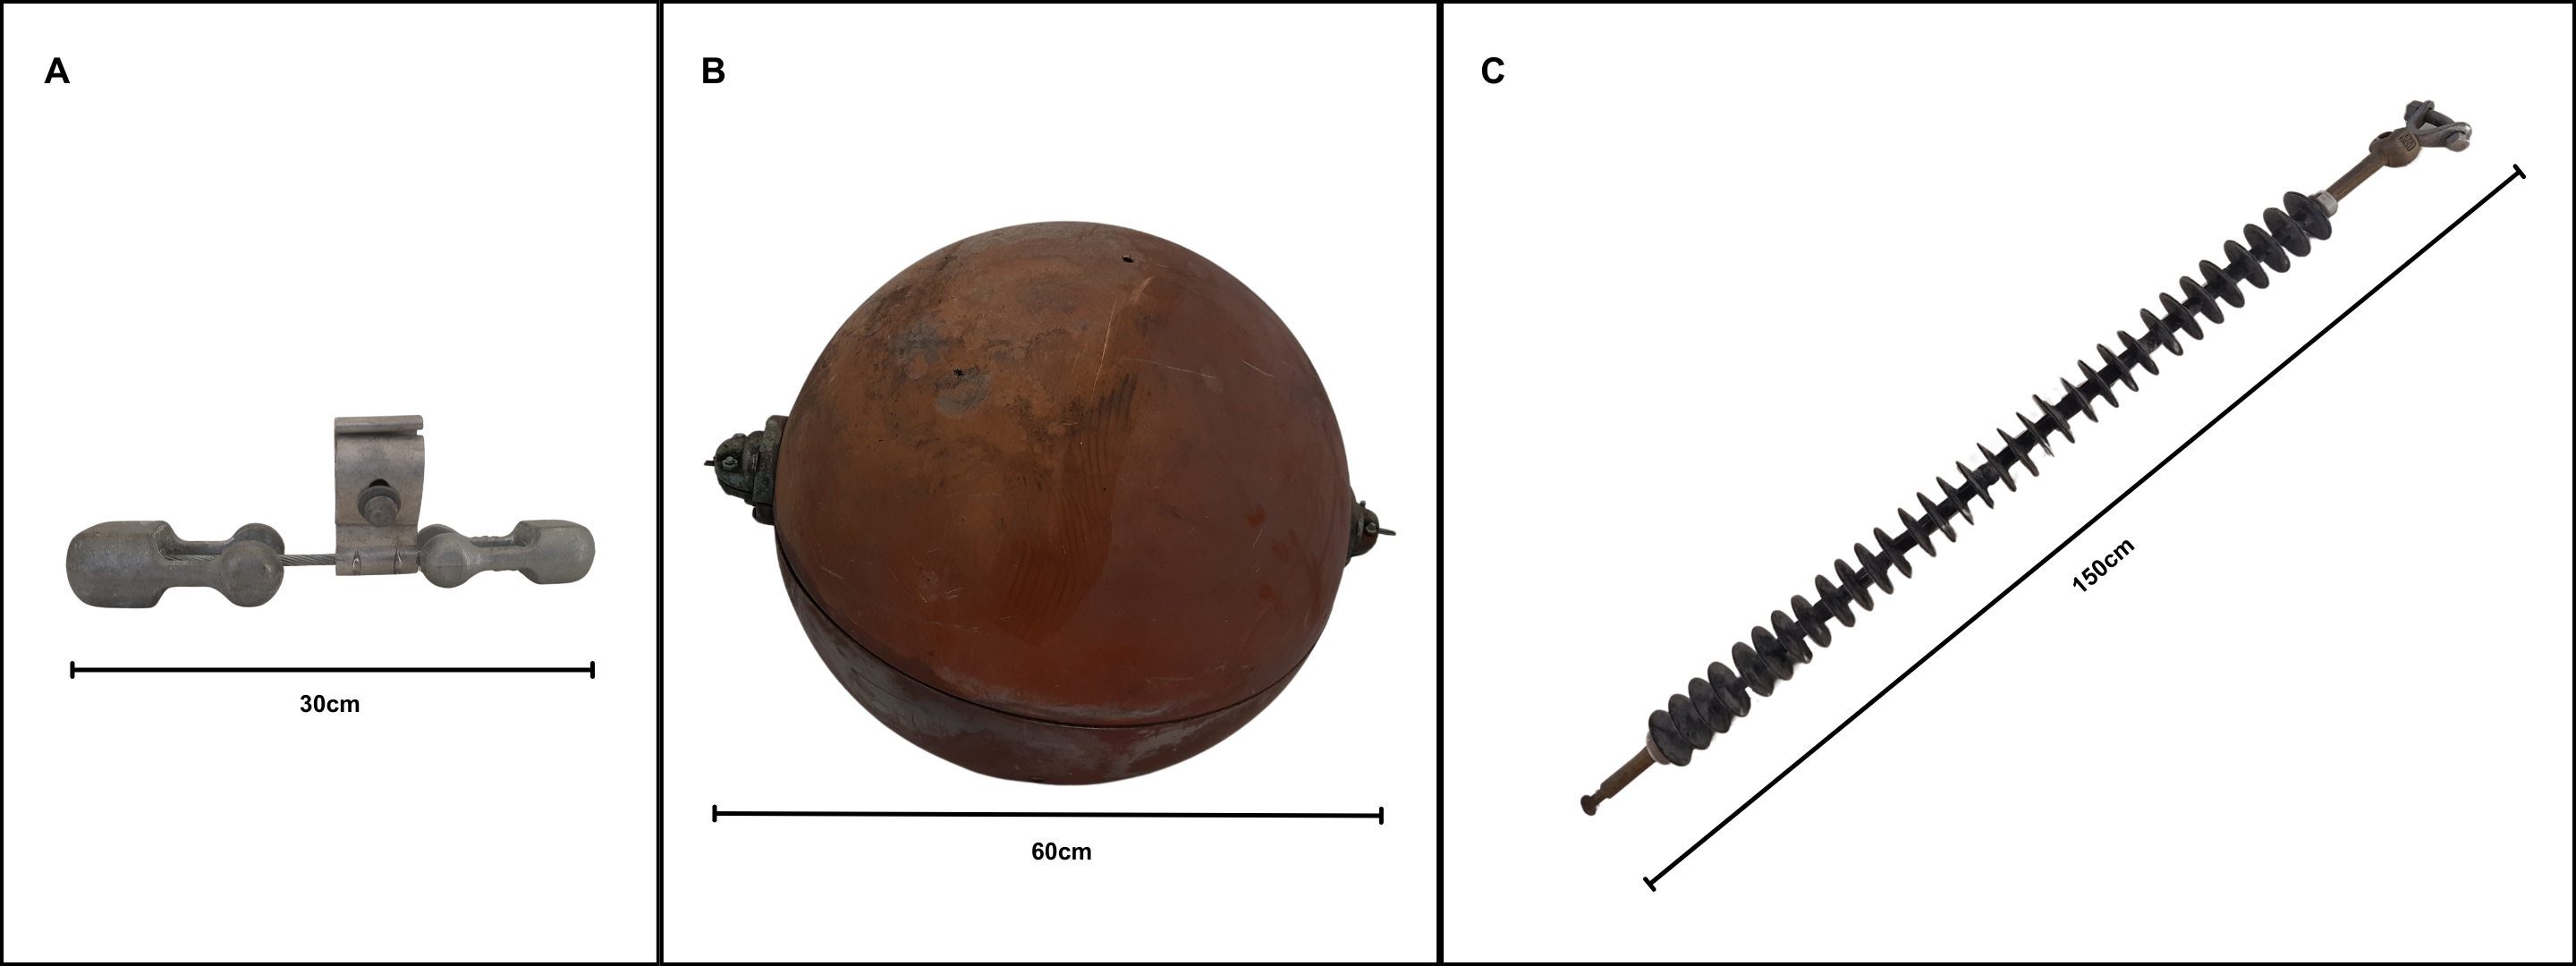
\includegraphics[width=0.8\textwidth]{Objetos.png} 
%     \caption{Objetos a Serem Detectadas}
%     \label{fig:classes_objetos}
% \end{figure}

% \begin{figure}[h]
%         \centering
%         \includegraphics[width=0.8\textwidth]{ObjetosSimu.png} 
%         \caption{Objetos a Serem Detectadas (Simulação)}
%         \label{fig:classes_objetos}
%     \end{figure}

\subsection{Sensores utilizados}

Neste projeto, foram utilizados dois tipos de sensores: o LiDAR e a câmera de profundidade. O LiDAR funciona emitindo feixes de luz laser que são refletidos pelos objetos ao seu redor. A partir do tempo que o feixe leva para retornar ao sensor, é possível calcular a distância até o objeto com alta precisão. Ele gera um valor de distância para cada ângulo de varredura, cobrindo um campo de visão de 360º, o que permite mapear a estrutura tridimensional do ambiente de forma eficiente. Já a câmera de profundidade utiliza luz infravermelha para gerar um mapa denso de profundidade, capturando a distância de cada ponto em sua linha de visão. Diferentemente do LiDAR, que mede distâncias pontuais a partir de um feixe, a câmera de profundidade fornece uma imagem completa com a informação de distância de cada pixel.

\subsection{Planejamento da Coleta de Dados}

A coleta de dados neste trabalho foi planejada com o objetivo de gerar uma base diversificada e representativa de amostras que permitisse o treinamento eficaz de modelos de aprendizado de máquina para a classificação de objetos em linhas de transmissão. Para isso, buscou-se capturar diferentes características espaciais dos objetos de interesse, considerando variações de distância. Foram utilizados dois tipos de sensores de profundidade, de modo a enriquecer a base com diferentes perspectivas e formatos de dados. A coleta foi realizada em dois cenários distintos, um simulado e outro real, seguindo um protocolo padronizado de captura de múltiplas amostras por objeto. Em ambos os cenários, será coletado um total de 150 instâncias de dados para cada tipo de objeto, totalizando um número significativo de amostras que ajudam na robustez do modelo de aprendizado. Cada instância corresponde a uma varredura de 360º realizada pelo LiDAR, bem como uma imagem capturada pela câmera de profundidade, com cada amostra variando em relação à distância do robô aos objetos, e consequentemente, a distância entre os sensores e os mesmos. Os dados foram organizados e rotulados de forma a permitir sua posterior divisão em conjuntos de treinamento, validação e teste. 

A base de dados coletada neste trabalho é crucial para o treinamento dos modelos de aprendizado de máquina, pois sua riqueza em informações determina diretamente a eficácia e precisão da classificação dos objetos. Quanto mais diversificada e representativa for a base de dados, mais robusto e preciso será o modelo treinado, ainda que o treinamento se torne mais intenso e demorado devido ao volume de dados. O objetivo principal da coleta é capturar as características espaciais dos objetos de interesse. Espera-se que os sensores de profundidade possam extrair informações detalhadas sobre a geometria dos objetos, suas dimensões, e suas posições relativas dentro do ambiente de inspeção. Esses dados são essenciais para permitir uma classificação precisa e eficiente dos diferentes tipos de objetos encontrados durante a inspeção das linhas de transmissão.

\subsection{Organização e Formato dos Dados Coletados}

Para possibilitar o uso eficiente dos dados capturados no treinamento e validação dos modelos de aprendizado de máquina, adotou-se uma estrutura de armazenamento clara e padronizada. Os dados do sensor LiDAR foram armazenados em arquivos \textit{CSV} (Comma-Separated Values), e os dados da câmera de profundidade foram salvos em imagens no formato \textit{PNG} (Portable Network Graphics), ambos amplamente compatíveis com bibliotecas de processamento. Além disso, cada amostra foi acompanhada por metadados como rótulo da classe, origem (simulado ou real) e timestamp, assegurando organização e rastreabilidade.

No caso do LiDAR, cada arquivo CSV contém 150 leituras, correspondendo a 150 amostras capturadas em diferentes distâncias entre o robô e o objeto. Cada linha representa uma leitura completa, e cada coluna corresponde a um ângulo fixo dentro do campo de visão de 360°, com os valores expressando distâncias em metros (até 12 m). A estrutura tabular simplifica o processamento e permite fácil inspeção e depuração, além de possibilitar sincronização com os dados da câmera.

As imagens da câmera de profundidade foram salvas em escala de cinza, com codificação ajustada conforme a origem dos dados. Para as imagens obtidas na simulação, os valores de cada pixel foram representados por inteiros sem sinal de 8 bits, totalizando uma escala de 0 a 255. Cada valor nessa escala foi linearmente associado a uma distância entre 0 e 10 metros, permitindo a reconstrução aproximada da profundidade observada em cada ponto da imagem. Já para a câmera real, os valores de pixel foram salvos utilizando inteiros sem sinal de 16 bits, com valores de 0 a 65.535. Nesse caso, a correspondência entre o valor do pixel e a distância é direta: cada unidade representa um milímetro de distância entre o objeto e o sensor. Em ambos os casos, a resolução da câmera foi mantida em 1280 × 720 pixels, garantindo consistência na estrutura dos dados para posterior processamento.

Para assegurar a correta associação entre sensores e objetos, cada leitura foi feita com apenas um objeto presente no campo de visão, o que elimina ambiguidades na rotulagem. Os dados foram organizados em pastas hierárquicas: o diretório principal indica a origem (\textit{real} ou \textit{simulado}) e contém subpastas nomeadas conforme o tipo de objeto (amortecedor, isolador, sinalizador ou nenhum), o que facilita a navegação e o uso por scripts automatizados.

\subsection{Ferramentas e Scripts de Coleta}

A aquisição dos dados foi conduzida por meio de scripts desenvolvidos em Python~\cite{python}, integrados ao ROS para gerenciar a comunicação entre os componentes do sistema. Esses scripts eram responsáveis por subscrever os tópicos dos sensores LiDAR e da câmera de profundidade, controlar o fluxo de aquisição e salvar os dados de forma sincronizada.

Para manipulação e organização dos dados, foram empregadas bibliotecas amplamente utilizadas na comunidade científica. O \textit{NumPy}~\cite{2020NumPy-Array} foi utilizado para processar vetores numéricos com eficiência, enquanto o \textit{Pandas}~\cite{mckinney2010data} facilitou a estruturação e exportação dos dados em arquivos \textit{CSV}. Para as imagens de profundidade, a biblioteca \textit{OpenCV}~\cite{opencv_library} foi utilizada na conversão e salvamento das imagens no formato \textit{PNG} em escala de cinza, conforme os padrões de codificação descritos anteriormente.

A coleta foi automatizada por meio de um loop de captura controlado, no qual cada iteração realizava a aquisição simultânea dos dados dos dois sensores. Entre as capturas, o robô era deslocado progressivamente em direção ao objeto alvo, com a distância de movimentação variando conforme o tipo de objeto analisado. Isso permitiu a obtenção de amostras com diferentes distâncias, aumentando a diversidade e representatividade da base de dados.

Para garantir a integridade e rastreabilidade dos dados, implementou-se também um sistema de registro de logs. Esse sistema armazenava informações como timestamp das amostras, falhas na leitura e inconsistências detectadas. Leituras fora do padrão esperado, como arquivos corrompidos, valores nulos ou discrepantes, foram automaticamente sinalizadas e descartadas.

Essa abordagem automatizada e monitorada proporcionou uma coleta de dados robusta, consistente e reprodutível, minimizando a intervenção manual e otimizando o tempo necessário para aquisição.

\subsection{Pré-processamento Inicial}

Devido ao funcionamento do sensor LiDAR, que realiza leituras em 360°, foi necessário filtrar os dados para considerar apenas os ângulos relevantes ao projeto, uma vez que essa configuração não pode ser alterada diretamente via hardware ou firmware. Assim, durante a captura, são selecionados apenas os valores correspondentes à faixa angular de interesse.

Já as imagens capturadas pela câmera de profundidade não passaram por pré-processamento antes do salvamento, pois os dados foram armazenados diretamente no formato esperado para as etapas subsequentes.

\subsection{Considerações Éticas e Reprodutibilidade}

O processo de coleta de dados foi planejado para garantir que outros pesquisadores possam replicar os experimentos e utilizar a base de dados gerada. Para isso, toda a metodologia, configurações dos sensores, scripts de aquisição e construção dos cenários simulados foram documentados detalhadamente. Além disso, os dados coletados e os datasets construídos estão disponíveis para acesso público no seguinte endereço: \href{https://drive.google.com/drive/folders/15SVMC3oxSVKuzv5S0CRKXIKJzF0k-9lz?usp=sharing}{Datasets}. 

O objetivo é que o projeto seja totalmente replicável, ou que seus dados possam ser reutilizados em trabalhos futuros, mediante solicitação prévia para fins de colaboração ou desenvolvimento.

Quanto à qualidade dos dados, foram aplicados filtros para eliminar valores aberrantes ou muito discrepantes durante as aquisições. As rotulações foram cuidadosamente revisadas para evitar erros de classificação. A quantidade de amostras para cada tipo de objeto é considerada suficiente para o escopo deste trabalho, cobrindo variações realistas de distância entre os sensores e os objetos.

Entretanto, é importante destacar que, apesar dos cuidados adotados, algumas fontes de viés podem estar presentes nos dados. Por exemplo, a coleta realizada em ambientes controlados, tanto simulados quanto reais, pode não contemplar todas as variações e ruídos presentes em situações operacionais reais. Além disso, a escolha dos objetos e das distâncias pode influenciar a representatividade dos dados para outros cenários. Reconhecer essas limitações é fundamental para a correta interpretação dos resultados e para orientar futuros trabalhos de validação e expansão da base.

\section{Construção das Cenas Simuladas}

Nesta seção são apresentados os procedimentos adotados para a criação das cenas simuladas no ambiente virtual, essenciais para a coleta controlada dos dados utilizados no treinamento e validação dos modelos de classificação. A simulação permitiu a definição precisa da configuração espacial dos sensores e dos objetos de interesse, a experimentação ágil de diferentes cenários e parâmetros, além de garantir segurança e redução de custos ao evitar o desgaste e riscos associados à operação em ambientes reais. Os detalhes da modelagem, posicionamento dos sensores, controle do robô simulado e integração com o ROS serão detalhados nas subseções seguintes, assim como o protocolo de coleta e as limitações inerentes ao uso da simulação.

\subsection{Ambiente Virtual Criado no CoppeliaSim}

A estrutura geral da cena simulada consistia em duas torres de transmissão posicionadas a 100 metros de distância uma da outra, conectadas por um cabo cilíndrico e retilíneo, sem curvaturas, a fim de simplificar a análise e evitar instabilidades na simulação. Os objetos de interesse foram pendurados ao longo do cabo, dispostos de forma que pudessem ser capturados individualmente pelos sensores. O robô foi posicionado sobre o cabo com liberdade de movimento linear, controlado pelo usuário por meio de comandos com velocidade ajustável. Os sensores foram acoplados a um suporte fixado no robô, permitindo sua movimentação ao longo da linha.

A modelagem dos componentes utilizados na simulação foi realizada por meio de uma combinação entre o software SolidWorks e os recursos nativos do CoppeliaSim. Os modelos dos robôs foram inicialmente criados no SolidWorks, o que possibilitou uma construção geométrica precisa. Posteriormente, foram exportados para o CoppeliaSim, onde as partes dinâmicas dos robôs foram substituídas por formas primitivas, como cubos e cilindros, a fim de garantir maior leveza e estabilidade na simulação sem comprometer a fidelidade das interações físicas.

Os objetos de interesse para classificação — amortecedores, isoladores e sinalizadores — bem como as torres, também foram modelados no SolidWorks e importados integralmente para o simulador. Diferente do robô, esses elementos mantiveram suas formas completas, pois era essencial preservar suas características físicas e visuais para uma correta detecção e classificação pelos sensores. O cabo foi representado por um cilindro simples, evitando o uso de simulação de curvatura realista, que poderia sobrecarregar o ambiente.

Para assegurar a portabilidade do sensor multimodal (LiDAR e câmera de profundidade) entre diferentes plataformas robóticas, foi desenvolvido um suporte específico no SolidWorks, projetado para manter os sensores corretamente alinhados e fixos. Esse suporte foi integrado ao robô no ambiente do CoppeliaSim, e pode ser facilmente adaptado a diferentes topologias robóticas, permitindo testes variados com o mesmo conjunto de sensores.

A complementaridade dos sensores utilizados está diretamente relacionada à sua posição no robô: a câmera de profundidade foi posicionada na parte superior, oferecendo uma visão panorâmica da porção superior do cabo e dos objetos suspensos, enquanto o LiDAR foi instalado abaixo do robô, capturando dados da região inferior. A combinação dessas perspectivas amplia a qualidade e a riqueza dos dados obtidos, fornecendo uma visão tridimensional mais completa dos componentes inspecionados nas linhas de transmissão.

\subsection{Robô Simulado}

Neste projeto, foram utilizados três protótipos de robôs simulados com o objetivo principal de testar a portabilidade e a adaptabilidade do suporte de sensores entre diferentes topologias robóticas. No entanto, apenas um desses robôs foi utilizado para a coleta dos dados de treinamento dos modelos, enquanto os outros dois serviram para validar o desempenho dos modelos em estruturas distintas.

O robô utilizado na fase de treinamento é o mais simples dos três. Sua estrutura é composta por um suporte de sensores posicionado de forma perpendicular ao cabo e alinhado ao corpo do robô. Ele possui um mecanismo de travamento que permite sua fixação ao cabo e é capaz de realizar deslocamentos lineares com velocidade ajustável, controlada via ROS. A simplicidade desse modelo favorece maior estabilidade durante a coleta de dados, reduzindo variáveis que poderiam interferir nos resultados.

Os dois robôs adicionais apresentam maior complexidade estrutural e foram projetados para superar obstáculos presentes nas linhas de transmissão. Nesses modelos, o suporte dos sensores foi instalado com uma leve inclinação em relação ao corpo principal do robô, simulando diferentes ângulos de visualização. Ambos mantêm o mesmo sistema de controle via ROS, com velocidades lineares também ajustáveis por código, permitindo comparações consistentes com o modelo mais simples.

A construção dos sistemas robóticos foi inteiramente baseada em juntas rotacionais simples disponibilizadas pelo CoppeliaSim. Essas juntas simulam movimentos giratórios básicos e, quando combinadas, possibilitam a reprodução de movimentos mais complexos. Todas as juntas foram integradas ao ROS, o que facilitou a implementação e o controle. Essa abordagem modular e padronizada simplifica o desenvolvimento e a replicação do sistema em diferentes configurações robóticas.

\subsection{Integração com ROS}

A integração entre o ambiente de simulação CoppeliaSim e o sistema ROS foi realizada por meio de scripts escritos em Lua diretamente no simulador. Cada objeto da cena recebe um identificador único no script, o que permite controlar suas propriedades diretamente. No caso de juntas, por exemplo, é possível configurar parâmetros como torque e velocidade.

Utilizando a biblioteca integrada do ROS fornecida pelo CoppeliaSim, foram implementados publicadores e assinantes diretamente nos scripts em Lua. Essa comunicação permite que o simulador interaja em tempo real com o ROS rodando na máquina. As juntas do robô foram controladas por assinantes que recebiam comandos externos, gerados por um código fora do ambiente CoppeliaSim, sob controle do usuário. Por outro lado, os sensores, como a câmera de profundidade e o LiDAR, funcionaram como publicadores, transmitindo dados para seus respectivos tópicos definidos no script de simulação. Esses dados eram então capturados por outro código externo responsável por processá-los e armazená-los para uso posterior.

Para garantir a confiabilidade da integração e dos dados utilizados nos experimentos, foram realizados testes de validação. Objetos foram posicionados a distâncias conhecidas dos sensores, permitindo verificar a acurácia dos dados de profundidade publicados. Além disso, foi verificada a sincronização temporal e espacial entre os sensores antes do início da coleta definitiva dos dados, assegurando que as leituras fossem consistentes e alinhadas para uso no treinamento dos modelos de classificação.

\subsection{Protocolo de Coleta na Simulação}

Para realizar a coleta de dados nas cenas simuladas, os objetos foram posicionados individualmente à frente dos sensores do robô. O controle do robô foi feito manualmente pelo usuário, que o aproximava dos objetos até que o sensor LiDAR detectasse sua presença. A partir desse momento, era iniciada a gravação dos dados, enquanto o robô se deslocava em direção ao objeto com velocidade constante.

A velocidade de deslocamento foi configurada de forma distinta para cada objeto, levando em consideração suas dimensões. Objetos menores, por exemplo, exigiram velocidades menores para garantir uma quantidade suficiente de amostras, de modo a equilibrar o volume de dados coletado em relação aos objetos maiores.

Após a coleta, os dados passaram por um processo de inspeção para a identificação e remoção de valores discrepantes ou incoerentes. Caso necessário, o processo de aquisição era repetido, a fim de garantir que os dados representassem com fidelidade o objeto analisado. Os dados finais foram então organizados e armazenados de maneira estruturada, incluindo os rótulos correspondentes a cada classe de objeto, para posterior uso no treinamento e avaliação dos modelos de aprendizado de máquina.

\subsection{Limitações e Considerações sobre a Simulação}

A simulação apresenta algumas limitações em relação ao ambiente real, principalmente no que diz respeito à fidelidade das leituras dos sensores. Nos ambientes simulados não há presença de ruídos, reflexos ou deformações nos dados capturados, o que favorece a obtenção de informações limpas e consistentes. No entanto, essa ausência de imperfeições pode comprometer a generalização dos modelos treinados exclusivamente com dados simulados, uma vez que sensores reais estão sujeitos a reflexos, interferências e variações físicas nas medições.

Como ambos os sensores utilizados operam por meio da emissão de feixes de luz (infravermelho), o fator que mais impacta a qualidade das medições no mundo real são as reflexões em superfícies irregulares ou brilhantes. Essa característica não é reproduzida na simulação, pois o CoppeliaSim não modela o comportamento real dos feixes de luz nem as propriedades ópticas dos materiais simulados.

Apesar dessas limitações, a simulação desempenha um papel fundamental como etapa preliminar do desenvolvimento. Ela permite gerar conjuntos de dados organizados, com classes bem definidas e isentas de ruído, que são extremamente úteis para a validação inicial dos modelos de aprendizado de máquina. Além disso, os resultados obtidos com dados simulados servem como base de comparação para os modelos treinados com dados reais, oferecendo uma referência inicial sobre o desempenho esperado e facilitando a análise das discrepâncias entre os dois contextos.

\section{Construção das Cenas no Laboratório}

Após a etapa de simulação, torna-se essencial validar o desempenho do sistema em condições reais, onde as limitações dos sensores e os desafios do ambiente físico podem impactar diretamente a eficácia dos modelos desenvolvidos. Esta seção descreve o processo de construção das cenas no laboratório, utilizado como ambiente de testes controlado para replicar, em escala reduzida, os elementos principais de uma linha de transmissão de energia. O objetivo é analisar a robustez do sistema diante de variações naturais e ruídos típicos dos sensores reais, bem como avaliar a viabilidade prática da solução proposta. Serão abordadas desde a infraestrutura física do laboratório, passando pela montagem do protótipo e do cabo suspenso, até os métodos de coleta e gerenciamento dos dados em ambiente real. A integração com o ROS, a comunicação embarcada e a adaptação dos scripts desenvolvidos na simulação para a coleta física também são discutidas, permitindo uma comparação direta entre os dados simulados e reais.


\subsection{Objetivos da Validação em Ambiente Real}

A validação em ambiente real tem como principal finalidade confirmar a viabilidade prática do sistema desenvolvido, observando o comportamento dos sensores físicos e do robô em condições controladas, porém reais. Por meio desses testes, é possível identificar limitações operacionais dos sensores, como perdas de dados por reflexões, ruídos de leitura e falhas na aquisição, que não estão presentes na simulação. Além disso, essa etapa permite avaliar a robustez dos modelos de classificação quando expostos a variações naturais no ambiente, garantindo que o desempenho observado virtualmente possa ser replicado, ao menos em parte, no cenário físico. A coleta em laboratório representa, portanto, um elo essencial entre o ambiente idealizado da simulação e as futuras aplicações operacionais do sistema em campo.

\subsection{Infraestrutura do Laboratório}

Os testes em ambiente real foram realizados em um laboratório com infraestrutura necessária para a montagem de uma linha de transmissão em escala reduzida, bem como para a construção e operação dos protótipos robóticos utilizados no projeto. O espaço físico disponível permitia a instalação de um cabo suspenso com cerca de 5 metros de comprimento, fixado a aproximadamente 2 metros do solo, proporcionando um ambiente controlado e representativo para a realização dos experimentos.

A sustentação do cabo foi viabilizada por meio de suportes metálicos do tipo cotovelo, fixados diretamente às paredes laterais do laboratório. O cabo foi preso aos suportes utilizando abraçadeiras de aço, garantindo rigidez e leve afundamento central, simulando a curvatura natural de cabos em linhas reais. Essa configuração permitiu a instalação segura dos objetos de interesse e possibilitou o deslocamento contínuo do robô ao longo do trecho durante as coletas.

\subsection{Coleta com Robô em Cabo Suspenso}

O robô utilizado nas coletas em ambiente real é uma réplica funcional do modelo empregado nas simulações virtuais. Trata-se de um protótipo móvel desenvolvido para se deslocar linearmente sobre um cabo suspenso, com capacidade de ajuste de velocidade e mecanismos de travamento e destravamento, garantindo segurança e estabilidade durante a movimentação e a aquisição dos dados.

O sistema de locomoção é composto por dois motores de passo: um responsável pelo deslocamento linear ao longo do cabo e outro dedicado ao acionamento do mecanismo de travamento. Ambos os motores são controlados por um microcontrolador Arduino, que atua como interface entre o hardware e o ROS, permitindo a reutilização do mesmo código e lógica de controle aplicados na simulação. A estrutura completa do robô e seu funcionamento detalhado podem ser consultados em \citeonline{10.1007/978-3-031-58676-7_42}.

O controle e a alimentação do sistema são realizados por uma Raspberry Pi 5, que se comunica com o Arduino e com os sensores (LiDAR e câmera de profundidade) por meio de interfaces seriais. Toda a alimentação elétrica é provida por baterias embarcadas, tornando o sistema completamente autônomo e dispensando conexões externas durante os testes.

\subsubsection{Estrutura do cabo suspenso}

A estrutura do experimento consiste em um cabo de alumínio com alma de aço (ACSR — Aluminium Conductor Steel Reinforced), similar aos utilizados em linhas de transmissão reais. O cabo, com cerca de 5 metros de comprimento, foi suspenso a uma altura aproximada de 2 metros do solo, fixado nas extremidades por meio de suportes metálicos do tipo cotovelo ancorados nas paredes do laboratório. A fixação foi feita com abraçadeiras de aço, garantindo estabilidade e uma leve curvatura natural do cabo.

Os objetos de interesse — como isoladores, amortecedores e sinalizadores — foram fixados ao cabo individualmente durante os testes. Os componentes utilizados são peças reais, idênticas às aplicadas em linhas de transmissão de alta tensão, e foram montados utilizando os mesmos métodos de fixação empregados em campo, assegurando uma representação fidedigna do ambiente operacional.

\subsection{Integração com ROS}

Para a integração dos sensores e atuadores no ambiente real, o ROS é executado diretamente na Raspberry Pi 5 embarcada no robô. A Raspberry atuou como nó mestre, sendo responsável pela orquestração e processamento de todas as informações do sistema. No entanto, ela não possui suporte nativo aos sistemas operacionais Ubuntu 20.04 ou Debian 10, os quais são requisitos para o ROS Noetic — versão escolhida para este projeto. Para contornar essa limitação, optou-se pelo uso do Docker, uma plataforma de virtualização leve baseada em contêineres que permite a execução isolada de aplicações em qualquer sistema operacional compatível~\cite{merkel2014docker}.

O contêiner Docker foi configurado com permissões equivalentes ao usuário root do sistema, garantindo acesso irrestrito a portas seriais e arquivos do dispositivo. Dentro desse contêiner, o ambiente ROS foi completamente configurado, incluindo os nós responsáveis por publicar os dados dos sensores e comandar os motores.

O controle dos motores foi realizado por meio do pacote \textit{rosserial}, que provê uma interface de comunicação entre dispositivos embarcados, como o Arduino, e o ROS, permitindo a publicação e subscrição de tópicos por meio de uma conexão serial~\cite{rosserial}.

Para a câmera de profundidade fui utilizada a Intel RealSense D415 com o pacote \textit{realsense-ros}, fornecido pela própria Intel. Esse pacote oferece \textit{launch files} e configurações prontas para a integração da câmera ao ROS, facilitando a captura e publicação dos dados de profundidade e cor~\cite{realsense_ros}.

O sensor LiDAR empregado foi o RPLIDAR A1, cuja integração foi realizada por meio do pacote \textit{rplidar\_ros}, disponibilizado pela Slamtec. O pacote contém arquivos de configuração específicos para cada modelo de sensor, incluindo parâmetros de calibração e tópicos de publicação compatíveis com o ROS~\cite{rplidar_ros}.

Com esses pacotes devidamente configurados e em execução no contêiner Docker, os dados brutos dos sensores passaram a ser publicados em tópicos ROS, estando assim disponíveis para subscrição e processamento por outros módulos do sistema.

A coleta dos dados foi realizada utilizando os mesmos scripts empregados na fase de simulação, garantindo consistência e sincronização entre os sensores. Os dados adquiridos foram armazenados localmente na Raspberry Pi durante as sessões de coleta e, posteriormente, transferidos para uma estação de trabalho dedicada, onde foram utilizados para o treinamento e validação dos modelos de classificação.

\subsection{Protocolo de Coleta no Laboratório}

A coleta de dados no ambiente real foi conduzida de forma similar à realizada na simulação. O robô foi posicionado de forma manual próximo a cada objeto até que se confirmasse a correta detecção e leitura pelos sensores. Em seguida, o robô foi configurado para se deslocar com velocidade constante ao longo do cabo, realizando a captura dos dados sensoriais.

Cada objeto foi analisado individualmente, sendo necessário ajustar a velocidade do robô para cada caso, de modo a garantir a qualidade da leitura — assim como foi feito na fase de simulação. A velocidade foi escolhida de forma que os sensores pudessem capturar uma quantidade suficiente de amostras com o objeto dentro do campo de visão.

Após a coleta, os dados foram inspecionados manualmente para remoção de valores discrepantes ou amostras com ruídos excessivos. Esse processo garantiu que o conjunto final fosse conciso, representativo e estivesse devidamente rotulado, assegurando a integridade e a confiabilidade das informações utilizadas no treinamento e validação dos modelos de aprendizado de máquina.

\subsection{Comparação com a Simulação}

Os dados coletados com os sensores reais apresentaram níveis de ruído, como era esperado, mas de forma geral mantiveram boa qualidade quando comparados aos dados da simulação, especialmente na análise de objetos com superfícies não reflexivas. Nesses casos, as leituras do LiDAR e da câmera de profundidade se mostraram consistentes e compatíveis com os dados simulados, validando a fidelidade do ambiente de simulação.

No entanto, ao lidar com objetos reflexivos, como o próprio cabo utilizado na estrutura, foram observadas distorções nas leituras. O LiDAR apresentou, em diversos momentos, medições no limite superior de alcance (cerca de 12 metros), especialmente nas primeiras e últimas amostras do objeto, quando os feixes eram emitidos em ângulos muito abertos em relação ao cabo. Tais valores são fisicamente impossíveis dentro do ambiente de teste — cujo teto estava a apenas 2 metros de altura — e indicam perda de dados devido à reflexão inadequada do feixe do sensor.

Já a câmera de profundidade demonstrou dificuldades ainda maiores nesse cenário. Durante toda a coleta, não foi possível obter leituras válidas de profundidade referentes ao cabo, mesmo em posições mais próximas. O sensor simplesmente atribuía o valor zero para esses pontos, indicando que a luz infravermelha não estava sendo refletida de forma adequada para que a profundidade pudesse ser estimada.

\section{Registro e Gestão dos Dados}

A organização dos arquivos gerados seguiu um padrão simples e funcional, dado que os dados foram coletados individualmente para cada objeto e devidamente rotulados no momento da aquisição. Isso evitou a necessidade de processos posteriores de separação ou balanceamento dos dados.

A nomenclatura adotada para os arquivos refletia diretamente o conteúdo dos dados, indicando o nome do objeto, o sensor utilizado (LiDAR ou câmera de profundidade) e a origem dos dados (simulação ou ambiente real). Essa padronização facilitou o processo de criação e manipulação dos \textit{datasets}.

Os dados utilizados para o treinamento dos modelos foram organizados em 10 \textit{datasets} distintos. As divisões foram feitas considerando:

\begin{itemize}
  \item Origem dos dados: simulado ou real;
  \item Tipo de sensor: apenas LiDAR, apenas câmera de profundidade ou ambos combinados;
  \item Forma de representação: dados brutos ou extração de \textit{features}.
\end{itemize}

Cada \textit{dataset} era composto por arquivos no formato \texttt{.csv}, contendo 150 amostras para cada uma das quatro classes de objetos (amortecedor, isolador, sinalizador, nada), totalizando 600 amostras por \textit{dataset}.

Além dos arquivos tabulares, foram criados dois \textit{datasets} adicionais com imagens de profundidade:

\begin{itemize}
  \item Um composto por imagens simuladas, obtidas diretamente do ambiente virtual;
  \item Outro composto por imagens reais, submetidas a técnicas de pré-processamento para remoção de ruído e aprimoramento da qualidade.
\end{itemize}

Esses conjuntos de imagens foram utilizados para o treinamento de uma rede neural convolucional, que serviu como \textit{benchmark} para avaliar a utilidade das informações visuais nas tarefas de classificação.


\section{Treinamento e Avaliação dos Modelos}

Esta seção descreve o processo de modelagem e avaliação dos algoritmos de aprendizado de máquina utilizados para a classificação de objetos em linhas de transmissão, com base em informações de profundidade coletadas por sensores. A motivação para o uso de técnicas de inteligência artificial neste contexto está na capacidade dessas abordagens de extrair padrões complexos dos dados, superando limitações de sistemas baseados apenas em regras ou análise manual. Ao treinar modelos supervisionados com os dados previamente rotulados, busca-se criar um sistema autônomo de classificação que seja robusto a variações dentro de um cenário real ou simulado.

\subsection{Objetivo da Etapa de Treinamento}

A etapa de treinamento tem como propósito utilizar os dados coletados — tanto simulados quanto reais — para desenvolver modelos capazes de classificar automaticamente os objetos encontrados ao longo de uma linha de transmissão, como isoladores, sinalizadores, amortecedores ou a ausência de objetos (classe “nada”). A modelagem visa permitir que, a partir das informações de profundidade fornecidas pelos sensores, seja possível inferir corretamente a classe do objeto observado.

\subsection{Arquiteturas e Algoritmos Testados}

Os modelos testados neste trabalho foram k-Vizinhos Mais Próximos (k-NN), Árvore de Decisão, Naive Bayes, Floresta Aleatória, Perceptron Multicamadas (MLP) e uma Rede Neural Convolucional (SqueezeNet), todos amplamente utilizados em tarefas de classificação. A seguir, descrevemos o funcionamento de cada modelo e seus principais hiperparâmetros, que impactam diretamente o desempenho e a capacidade de generalização. Para uma explicação mais aprofundada, consulte \cite{bishop2006pattern}.

\subsubsection{k-Vizinhos mais proximos}

O kNN é um modelo de aprendizado supervisionado que classifica um objeto com base na proximidade com exemplos já conhecidos no espaço de características. O princípio básico é encontrar os \textit{k} exemplos mais próximos (vizinhos) e decidir a classe do novo objeto segundo as classes desses vizinhos.

Os hiperparâmetros importantes do kNN incluem o número de vizinhos considerados, que define quantos exemplos próximos serão usados para a decisão, a métrica de distância, que determina como a proximidade entre pontos é calculada e pode influenciar a sensibilidade do modelo a diferentes características, e o esquema de pesos, que pode dar maior importância a vizinhos mais próximos.

\subsubsection{Árvore de Decisões}

A árvore de decisões utiliza uma estrutura hierárquica de perguntas sobre atributos dos dados para chegar a uma classificação final. Cada nó interno representa uma condição sobre um atributo e as folhas indicam a classe predita.

Os hiperparâmetros que controlam a árvore incluem a profundidade máxima, que limita o tamanho da árvore para evitar que ela se ajuste demais aos dados de treinamento (\textit{overfitting}), o número mínimo de amostras para dividir um nó, e o número mínimo de amostras para formar uma folha. Esses parâmetros ajudam a balancear a complexidade do modelo.

\subsubsection{Naive Bayes}

O Naive Bayes é um modelo probabilístico que assume independência condicional entre as características dado a classe. Ele calcula a probabilidade de cada classe dado o vetor de características e escolhe a mais provável.

Embora possua poucos hiperparâmetros, um deles é a escolha da distribuição probabilística usada para modelar os dados, como Gaussiana ou multinomial, o que afeta o cálculo das probabilidades condicionais e, consequentemente, o desempenho do modelo.

\subsubsection{Floresta Aleatória}

A Floresta Aleatória é um conjunto de árvores de decisão treinadas em subconjuntos aleatórios dos dados e características, cuja decisão final é feita por votação entre as árvores.

Os principais hiperparâmetros são o número de árvores no conjunto, que influencia a estabilidade e robustez da predição; a profundidade máxima das árvores; o número mínimo de amostras para dividir nós ou formar folhas; e o número máximo de características consideradas em cada divisão, que impacta a diversidade entre as árvores e ajuda a evitar \textit{overfitting}.

\subsubsection{Perceptron Multicamadas}

O MLP é uma rede neural feedforward composta por múltiplas camadas de neurônios totalmente conectados, capaz de modelar relações não lineares complexas entre as características e as classes.

Seus hiperparâmetros incluem a arquitetura da rede, ou seja, o número de camadas e neurônios por camada, que definem a capacidade de representação do modelo; a taxa de aprendizado, que afeta a velocidade e qualidade da convergência durante o treinamento; a função de ativação, que introduz não linearidade; e o número de épocas, que determina quantas vezes o conjunto de dados é usado para atualizar os pesos.

\subsubsection{Rede Neural Convolucional – SqueezeNet}

Além dos modelos clássicos, foi utilizada uma rede neural convolucional para classificação das imagens de profundidade capturadas pela câmera. A rede escolhida foi a SqueezeNet \cite{SqueezeNet}, que é conhecida por atingir acurácia comparável à AlexNet com um número muito menor de parâmetros e tamanho reduzido do modelo, facilitando sua implementação em sistemas embarcados.

A SqueezeNet é composta por blocos “fire”, que combinam camadas convolucionais de filtros pequenos (1x1) e maiores (3x3) para extrair características complexas das imagens de forma eficiente. Seus hiperparâmetros envolvem a configuração do número de filtros em cada camada, o tamanho dos filtros convolucionais, além dos parâmetros típicos de treinamento, como taxa de aprendizado, tamanho do lote (batch size) e número de épocas. Esperava-se que essa rede apresentasse desempenho superior em acurácia, ainda que com tempo de processamento maior que os modelos clássicos, sendo usada como referência para validação dos dados obtidos pela câmera de profundidade.

\subsection{Treinamento dos Modelos}

Os modelos foram treinados utilizando ferramentas robustas e amplamente adotadas na comunidade de aprendizado de máquina e aprendizado profundo. As principais bibliotecas utilizadas foram o \texttt{scikit-learn} e o \texttt{PyTorch}, ambas desenvolvidas em Python.

O \texttt{scikit-learn} é uma biblioteca de aprendizado de máquina de alto nível que oferece uma ampla variedade de algoritmos clássicos, incluindo kNN, árvores de decisão, Naive Bayes e Florestas Aleatórias, além de utilitários para pré-processamento, avaliação e seleção de modelos. Sua interface simples e eficiente facilita a implementação rápida de experimentos, sendo ideal para o treinamento e validação dos modelos clássicos usados neste trabalho \cite{pedregosa2011scikit}.

Já o \texttt{PyTorch} é uma biblioteca focada em aprendizado profundo, que proporciona um estilo imperativo de programação com alta performance e flexibilidade na construção de redes neurais, como a rede convolucional SqueezeNet utilizada neste projeto. Com suporte dinâmico para computação em GPU e funcionalidades avançadas para otimização e manipulação de tensores, o PyTorch permite o desenvolvimento e treinamento eficiente de modelos complexos \cite{NEURIPS2019_9015}.

Essas ferramentas complementares permitiram o desenvolvimento dos modelos clássicos e da rede neural convolucional, garantindo uma base sólida para o processo de treinamento e avaliação.

\subsection{Avaliação de Desempenho}

A avaliação dos modelos desenvolvidos foi realizada utilizando a técnica de validação cruzada, que consiste em dividir o conjunto de dados em subconjuntos para garantir uma análise mais robusta e menos enviesada do desempenho do modelo. Na validação cruzada, os dados são segmentados em múltiplas partições, onde, em cada iteração, um subconjunto é utilizado para teste enquanto os demais servem para treinamento. Esse processo é repetido até que todos os subconjuntos tenham sido usados como teste, e os resultados são então agregados para obter uma estimativa geral da performance.

A métrica escolhida para quantificar o desempenho dos modelos foi a acurácia, definida como a proporção de classificações corretas em relação ao total de amostras avaliadas. A acurácia é uma medida intuitiva e amplamente utilizada para problemas de classificação, pois indica diretamente a eficácia do modelo em reconhecer corretamente as classes presentes nos dados.

Além da avaliação tradicional, foi realizada uma validação específica para testar a capacidade dos modelos de generalizar entre diferentes configurações robóticas. Para isso, os modelos foram treinados utilizando um dataset obtido a partir de uma topologia robótica e validados em outro conjunto de dados capturado por uma topologia distinta. Essa abordagem visa avaliar a robustez do sistema frente a variações nas topologias de robôs inspetores.

O tempo gasto no processo de validação foi também monitorado, pois é um fator importante para aplicações em sistemas embarcados e em tempo real, onde a eficiência computacional é crítica para o funcionamento prático dos classificadores.

\subsection{Limitações da Metodologia}

A metodologia adotada neste trabalho apresenta algumas limitações importantes, principalmente relacionadas à coleta de dados reais para treinamento e validação dos modelos. Primeiramente, a coleta de dados reais está sujeita a restrições de espaço físico disponível no laboratório. O que impacta diretamente na representatividade e diversidade dos dados coletados.

No ambiente simulado, apesar de fornecer uma boa aproximação do cenário real de uma linha de transmissão, os sensores não sofrem interferências externas, como ruídos e reflexões, o que resulta em dados mais limpos e idealizados, que podem não refletir completamente as condições reais encontradas em campo.

Por outro lado, no ambiente de laboratório, os dados são capturados de sensores reais e, portanto, incluem reflexões e interferências típicas do mundo real, tornando-os mais concretos. Contudo, devido ao espaço físico limitado, o cenário representa apenas uma aproximação parcial das condições reais de uma linha de transmissão. Especificamente, o fundo de escala dos sensores nesse ambiente varia entre 2 e 5 metros, enquanto em uma estrutura real o fundo de escala pode alcançar até 12 metros, devido à ausência de objetos além da própria linha. Isso implica que as leituras obtidas no laboratório não reproduzem com fidelidade todas as características do ambiente real.

Além disso, por se tratar de um ambiente controlado, existe o risco de \textit{overfitting} dos modelos, isto é, os modelos podem apresentar bom desempenho nos dados utilizados para treinamento, mas ter baixa capacidade de generalização para situações não contempladas, como a presença de objetos inesperados na linha de transmissão ou variações significativas na posição dos objetos.

Essas limitações indicam a necessidade de futuras coletas de dados em ambientes reais e diversificados para melhorar a robustez e aplicabilidade dos modelos desenvolvidos.




%-----------------------------------------------------------%%% Comente para remover este item

%% Capítulo
%------------------------------------------------------------%

\chapter{Desenvolvimento}
\label{cap:trabalhos:desenvolvimento}

Este capítulo apresenta o desenvolvimento do sistema robótico proposto, abrangendo tanto os aspectos de hardware quanto os de software. Inicialmente, são descritas as características físicas e funcionais da plataforma robótica desenvolvida, incluindo alguns detalhes sobre a estrutura mecânica, os sensores embarcados e os sistemas de controle e comunicação utilizados. Também são apresentados os dois outros protótipos empregados durante as fases de simulação, com destaque para suas diferenças estruturais e contribuições ao processo de validação. Em seguida, é detalhada a configuração dos sensores no ambiente ROS, abordando os drivers utilizados, os parâmetros operacionais ajustados e as estratégias adotadas para formatar os dados obtidos em diferentes plataformas. Posteriormente, são explorados os aspectos de software, incluindo o controle do robô via ROS, o processamento e organização dos dados adquiridos e a implementação dos modelos de aprendizado de máquina. Todo o pipeline, desde a aquisição até a inferência em tempo real, foi projetado para ser modular, adaptável e compatível tanto com simulações quanto com a operação embarcada em plataformas reais.

\section{Hardware}

Esta seção descreve os aspectos físicos e estruturais do sistema robótico desenvolvido, incluindo detalhes da construção mecânica do robô utilizado para a coleta de dados reais, os protótipos testados em simulação, e a configuração do suporte dos sensores multimodais. São apresentados também os sensores utilizados e suas principais especificações técnicas.

\subsection{Estrutura Mecânica dos Robôs}

O robô utilizado na coleta de dados em ambiente real foi construído com estrutura impressa em 3D, baseada no mesmo modelo utilizado nas simulações desenvolvidas no CoppeliaSim. Seu deslocamento ocorre sobre um cabo rígido, representando uma linha de transmissão, e utiliza dois motores de passo: um responsável pelo deslocamento linear ao longo do cabo e outro para acionar o mecanismo de travamento/destravamento. Este mecanismo garante que o robô permaneça fixo ao cabo, impedindo quedas ou movimentos involuntários durante a coleta de dados.

Este modelo apresenta uma estrutura simplificada e não conta com sistemas embarcados para a superação de obstáculos. A escolha por este robô para a coleta de dados se deu por sua maior confiabilidade estrutural, sendo o mais estável dentre os disponíveis no laboratório. A proposta para uma versão final inclui a adição de um segundo conjunto de garra e um corpo robusto capaz de sustentar o robô com apenas uma garra acoplada. Em presença de obstáculos, a ideia é que o robô desacople uma das garras, rotacione-a para ultrapassar o obstáculo, recoloque-a no cabo após o objeto e, em seguida, repita o processo com a outra garra, garantindo a continuidade do deslocamento.

Além do protótipo utilizado na coleta real, dois outros robôs com mecanismos funcionais de superação de obstáculos foram projetados e simulados. O primeiro deles é composto por um corpo central com duas rodas laterais e uma garra central. Quando detecta um obstáculo, a garra se prende ao cabo, a roda dianteira se desacopla, desce, e o corpo do robô se estende para reposicionar a roda à frente do obstáculo. Após reposicionada, a roda retorna à altura do cabo, se fecha e o robô solta a garra, retrai o corpo e avança, repetindo o processo com a outra roda para completar a travessia do obstáculo.

O segundo robô possui três braços articulados, cada um equipado com rodas e um “cotovelo” acionável. Ao detectar um obstáculo, o primeiro braço eleva seu cotovelo e ultrapassa o obstáculo. Em seguida, os outros dois braços repetem o movimento sequencialmente, permitindo que o robô supere a barreira mantendo estabilidade e tração no cabo. Apesar da complexidade desses mecanismos, a instabilidade estrutural observada nos protótipos reais inviabilizou sua utilização na coleta física de dados, sendo restritos às simulações computacionais.

\subsection{Sensor Multimodal}

Para este projeto, foi construído um suporte físico com o objetivo de manter fixas a orientação e a posição dos sensores utilizados. O suporte foi projetado com o menor tamanho possível, desde que não comprometesse a estabilidade dos sensores. A escolha das posições relativas entre os sensores foi determinada com base em seus papéis específicos dentro do sistema robótico e nas exigências geométricas para uma coleta eficiente dos dados.

O sensor LiDAR tem como principal função levantar informações de profundidade ao redor da linha, sendo, portanto, essencial que ele possua uma visão desobstruída do ambiente. Para maximizar a utilidade das suas leituras, o plano de varredura do sensor deve estar livre de rotações em relação ao eixo da linha. Além disso, o ângulo do plano de leitura não pode ser muito próximo ao da própria linha, pois isso limitaria a abrangência das medições. Idealmente, o plano do LiDAR estaria orientado a $90^\circ$ em relação ao eixo do cabo, oferecendo uma visão lateral completa do entorno. No entanto, para que o robô seja capaz de detectar e classificar objetos à sua frente antes de se aproximar demasiadamente, é necessário inclinar o sensor em relação ao eixo do cabo. O melhor caso, nesse sentido, seria o sensor operando a $0^\circ$ em relação ao eixo do cabo, mirando diretamente à frente. (Figura para demonstrar?)

A câmera de profundidade também tem papel relevante na análise da linha e dos objetos presentes nela, sendo usada principalmente para detecção de possíveis danos físicos. Para evitar distorções e maximizar a qualidade das imagens, a câmera deve ser posicionada acima do cabo, com seu plano óptico perpendicular ao eixo da linha e voltado para frente.

Considerando os requisitos específicos de cada sensor, o suporte multimodal foi projetado para equilibrar as limitações de ambos. O ângulo de fixação do LiDAR foi definido como $45^\circ$ em relação ao eixo do cabo. Essa inclinação permite a coleta tanto de dados laterais quanto frontais, desde que o sensor esteja a uma distância horizontal adequada em relação ao cabo. A câmera foi posicionada na parte superior do robô, acima do cabo, a uma distância de $5\,\text{cm}$ a partir do centro do mesmo. (Figura com as medidas)

Foi estabelecido que a classificação dos objetos deve ser feita a partir da leitura combinada de ambos os sensores. Como a câmera de profundidade possui maior alcance visual em relação ao LiDAR (devido à sua posição elevada), definiu-se uma distância mínima de $40\,\text{cm}$ para a detecção e classificação de objetos. Ou seja, qualquer objeto a $40\,\text{cm}$ ou menos da frente do robô deve ser processado pelo sistema multimodal.

Para garantir essa faixa de detecção, o suporte foi projetado com $50\,\text{cm}$ de comprimento horizontal, mantendo o LiDAR a $45\,\text{cm}$ abaixo do cabo (a partir do seu centro) e a câmera a $5\,\text{cm}$ acima. Essa configuração assegura que o LiDAR possa detectar objetos a mais de $45\,\text{cm}$ de distância, caso estejam abaixo do cabo, e objetos a pelo menos $40\,\text{cm}$ se estiverem posicionados ligeiramente acima da linha. Dessa forma, o arranjo garante a eficácia do sistema de classificação sem comprometer a integridade ou a estabilidade do robô durante o deslocamento.

\subsection{Sensores Utilizados}

Para a realização deste projeto, foram selecionados dois sensores principais capazes de fornecer informações de profundidade complementares: a câmera Intel RealSense D415 e o LiDAR RPLIDAR A1M8. Ambos os sensores foram integrados ao sistema embarcado do robô para permitir a coleta de dados tridimensionais, usados para a tarefa de classificação de objetos sobre as linhas de transmissão. A escolha por sensores de profundidade com diferentes princípios de funcionamento — estereoscopia ativa e triangulação a laser — visa garantir robustez ao sistema em diferentes condições de iluminação, ângulos de incidência e posicionamentos relativos dos objetos. A seguir, são descritas as principais características técnicas de cada sensor.

\subsubsection{Intel RealSense D415}

A câmera de profundidade Intel RealSense D415 utiliza um sistema estereoscópico ativo para gerar mapas de profundidade com alta precisão. A tecnologia baseia-se na captura simultânea de imagens por duas câmeras infravermelhas, associadas a um projetor de padrões que melhora a detecção em superfícies com baixo contraste visual. Essa configuração permite estimar a profundidade por meio da disparidade entre os pares de imagens. O sensor é amplamente empregado em aplicações de robótica, visão computacional e automação, dada sua confiabilidade e facilidade de integração com plataformas embarcadas.

% \begin{figure}[!h]
%     \centering
%     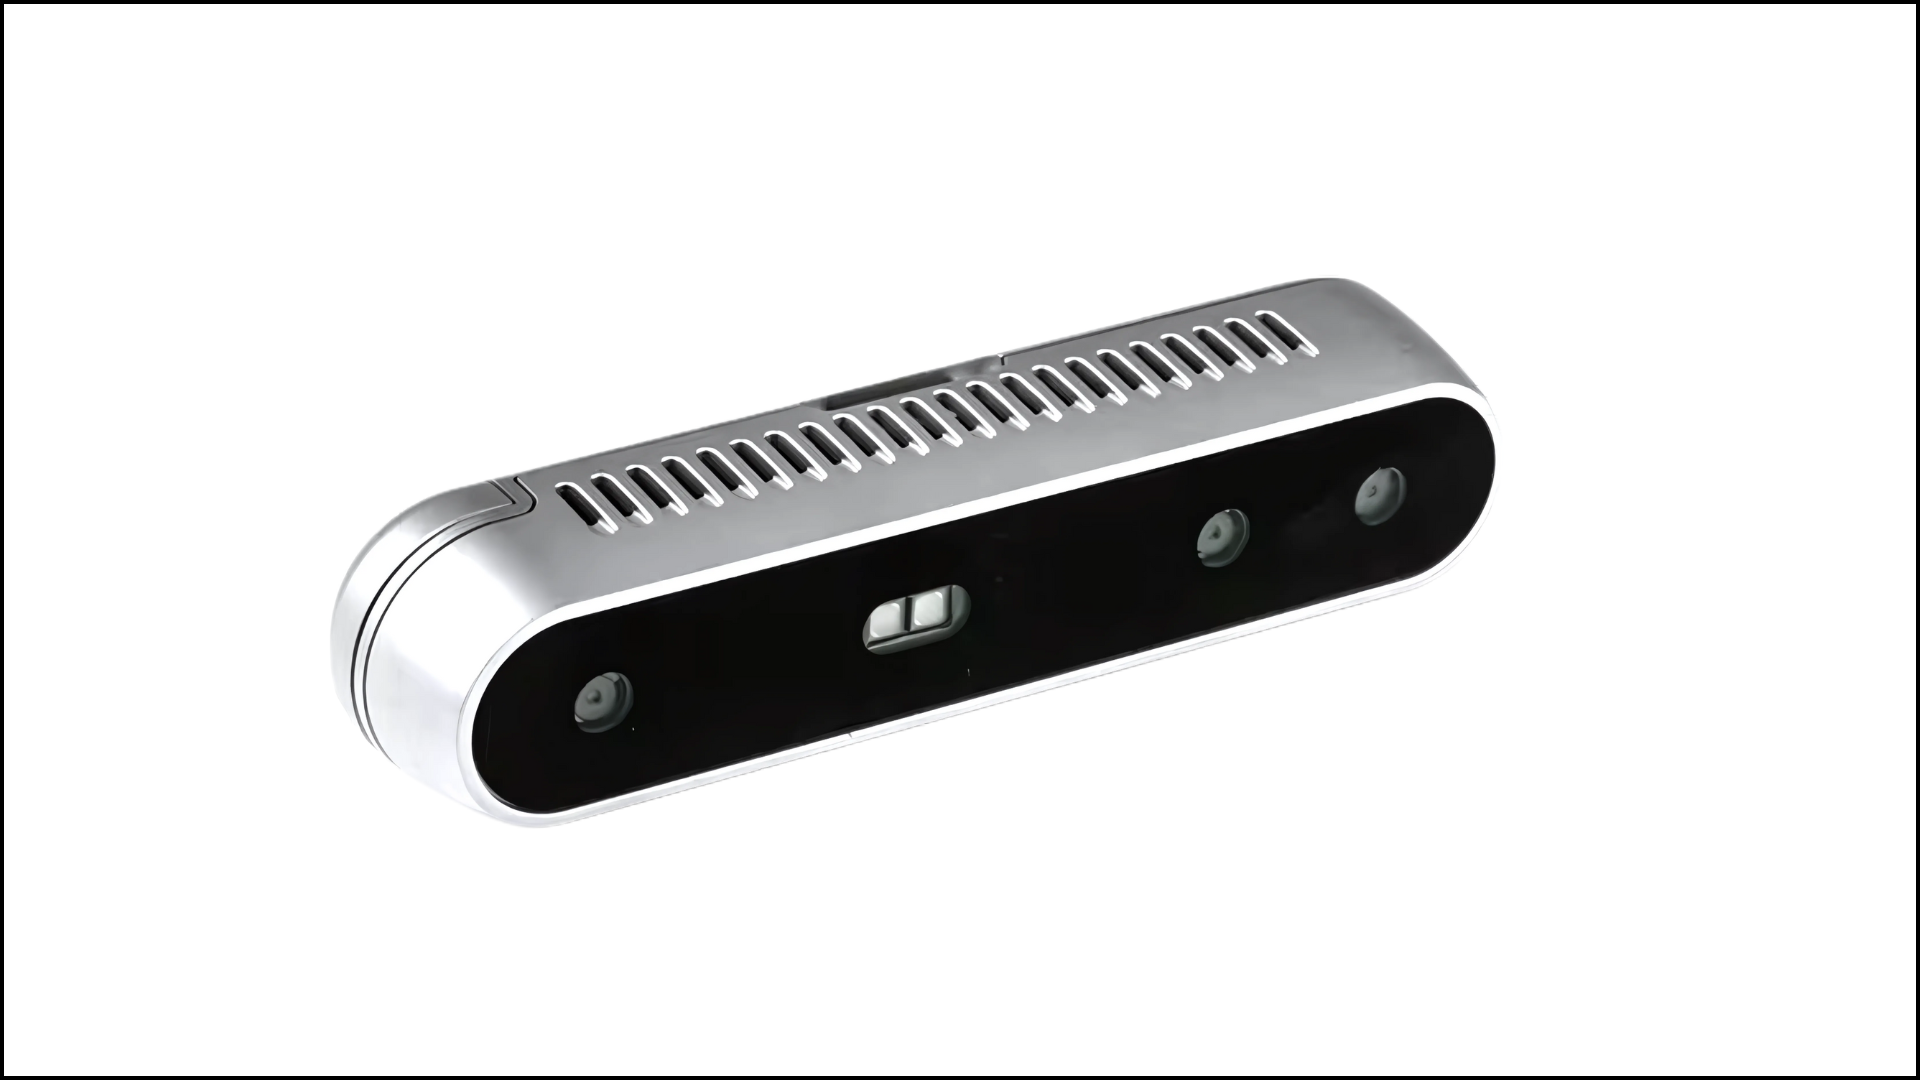
\includegraphics[width=0.4\columnwidth]{RealSense.jpg}
%     \caption{Intel RealSense D415}
%     \label{fig:realsense-D415}
% \end{figure}

As principais especificações técnicas da RealSense D415 incluem:

\begin{itemize}
    \item \textbf{Tecnologia de profundidade}: Estereoscopia ativa com projetor infravermelho
    \item \textbf{Distância mínima de operação}: Aproximadamente $0{,}45\,\text{m}$ para resolução máxima
    \item \textbf{Precisão de profundidade}: Erro inferior a $2\%$ a $2\,\text{m}$
    \item \textbf{Campo de visão (FOV)}: $65^\circ \times 40^\circ$
    \item \textbf{Resolução de saída}: Até $1280 \times 720$ pixels
    \item \textbf{Taxa de quadros (depth)}: Até $90\,\text{fps}$
\end{itemize}

\subsubsection{RPLIDAR A1M8}

O sensor RPLIDAR A1M8, desenvolvido pela Slamtec, é um sensor LiDAR de baixo custo que opera por meio da técnica de triangulação a laser infravermelho. Sua principal funcionalidade está na realização de escaneamentos 2D em $360^\circ$, sendo capaz de gerar nuvens de pontos com alta densidade. Devido à sua leveza, baixo consumo energético e boa precisão, o sensor é amplamente empregado em sistemas de navegação autônoma e mapeamento em tempo real (SLAM). Um motor rotativo interno aciona o movimento contínuo do feixe de laser, permitindo medições em tempo real com ampla cobertura angular.

As principais especificações técnicas do RPLIDAR A1M8 são:

\begin{itemize}
    \item \textbf{Tecnologia de medição}: Triangulação com laser infravermelho
    \item \textbf{Alcance de detecção}: $0{,}15\,\text{m}$ a $12\,\text{m}$
    \item \textbf{Campo de visão (FOV)}: $360^\circ$ contínuo
    \item \textbf{Frequência de varredura}: $10\,\text{Hz}$
    \item \textbf{Resolução angular}: $\leq 1^\circ$
    \item \textbf{Frequência de amostragem}: $\geq 8000$ pontos por segundo
    \item \textbf{Precisão de distância}: Erro inferior a $1\%$ da distância medida
    \item \textbf{Interface de comunicação}: UART (TTL $3{,}3\,\text{V}$)
\end{itemize}

\section{Firmware e Software}

O funcionamento do sistema proposto depende da integração eficiente entre o hardware embarcado, os sensores e os algoritmos de controle e aquisição de dados. Para isso, foi desenvolvido um conjunto de códigos em Python e C++ utilizando o framework ROS, que facilita a comunicação entre os diversos componentes do sistema. O firmware, executado na placa Arduino, é responsável apenas pela interface direta com os drivers dos motores, enquanto o software, executado na Raspberry Pi, gerencia os sensores, o controle dos atuadores e a coleta dos dados. As seções a seguir descrevem detalhadamente a configuração dos sensores, a estrutura de controle dos robôs, tanto em ambiente simulado quanto real, e o script de coleta e armazenamento dos dados utilizados no treinamento dos modelos de classificação.

\subsection{Controle do Robô via ROS}

O controle dos motores foi realizado por meio de um microcontrolador Arduino, que funcionou como interface entre o sistema ROS e os drivers dos motores. Para essa comunicação, foi criado um tópico específico no ROS, no qual as mensagens eram do tipo \texttt{std\_msgs/Int64MultiArray}. Cada posição do vetor representava um motor, e seu valor indicava, conforme a topologia do robô, a velocidade ou o número de passos a ser executado. O Arduino recebia os comandos por meio da porta serial e os repassava aos motores, sendo responsável apenas pela comunicação com os drivers. Nenhuma lógica de controle era executada no próprio Arduino, ficando essa tarefa completamente a cargo dos nós do ROS.

No robô utilizado para aquisição dos dados, existiam dois elementos principais de controle: a trava de segurança e o motor responsável pelo deslocamento linear ao longo da linha de transmissão. A trava recebia, por meio do vetor de controle, o número de passos necessários para travar e destravar o robô no cabo condutor. O motor de movimentação, por sua vez, recebia a velocidade desejada. O código de controle desenvolvido no ROS impedia que o robô iniciasse o movimento sem que a trava estivesse acionada, garantindo a segurança da estrutura e prevenindo quedas.

Para os robôs utilizados nas simulações, foram adotados os mesmos códigos utilizados no robô físico, com adaptações no tamanho do vetor de controle para refletir o número de atuadores presentes em cada topologia. O robô simulado utilizado na aquisição de dados operava de forma idêntica ao robô real, enquanto outras topologias simuladas apresentavam variações no número de motores ou atuadores, mantendo, contudo, o mesmo princípio de controle por meio de tópicos ROS e vetores de comandos.

\subsection{Configuração dos Sensores}

Na simulação, foram utilizados modelos de sensores que reproduzem as mesmas características dos sensores reais adotados na implementação prática. As configurações foram realizadas por meio das bibliotecas \texttt{rplidar\_ros} e \texttt{realsense2\_camera}, disponíveis no ecossistema do ROS. Para o LiDAR, não foram necessárias modificações adicionais, pois a configuração padrão já atendia aos requisitos do projeto. No caso da câmera RealSense D415, foi ajustada para operar a uma taxa de 10~Hz e com resolução de 1280$\times$720 pixels, de modo a sincronizar sua aquisição com o LiDAR. Essa configuração resultou em uma distância mínima de leitura de aproximadamente 4,5 centímetros.

Uma vez configurados e iniciados os respectivos nós dos sensores, os dados passaram a ser publicados nos tópicos definidos pelas bibliotecas. O sensor LiDAR publica mensagens do tipo \texttt{sensor\_msgs/LaserScan}, que consistem em uma estrutura padronizada para representar leituras de distância obtidas por varredura a laser. Essa mensagem contém informações como o ângulo inicial (\texttt{angle\_min}) e final (\texttt{angle\_max}) da varredura, o incremento angular entre medições (\texttt{angle\_increment}), a distância mínima (\texttt{range\_min}) e máxima (\texttt{range\_max}) detectáveis, e o vetor \texttt{ranges}, que armazena as distâncias medidas, em metros, para cada ângulo. Opcionalmente, o campo \texttt{intensities} pode conter dados referentes à intensidade do sinal refletido, útil para análise de propriedades ópticas dos objetos. O campo \texttt{header}, presente em todas as mensagens ROS, fornece informações de carimbo de tempo e identificação do sistema de coordenadas (\texttt{frame\_id}) associado à leitura.

Para os sensores de visão, como a câmera de profundidade RealSense, os dados são publicados em tópicos do tipo \texttt{sensor\_msgs/Image}. Essa mensagem carrega as imagens ou quadros de vídeo capturados e contém metadados como a resolução da imagem (\texttt{width} e \texttt{height}), o número de bytes por linha (\texttt{step}) e os dados brutos da imagem no campo \texttt{data}. A codificação dos pixels é especificada no campo \texttt{encoding}, com formatos comuns como \texttt{"rgb8"}, \texttt{"bgr8"}, \texttt{"mono8"} ou \texttt{"yuv422"}. O campo \texttt{is\_bigendian} informa a ordem dos bytes utilizada. Neste projeto, foram utilizadas imagens em escala de cinza (\textit{grayscale}), com codificação de 8 bits por pixel para os dados simulados e de 16 bits por pixel para os dados adquiridos em ambiente real.

\subsection{Script de Coleta}

O script de coleta de dados foi desenvolvido em \textit{Python}, com o objetivo de registrar as informações publicadas nos tópicos dos sensores utilizados. Para a câmera de profundidade, o script armazenava diretamente as imagens geradas, enquanto, para o LiDAR real, era aplicado um pré-processamento com a finalidade de restringir o campo de leitura do sensor.

Esse pré-processamento consistia em limitar o ângulo de leitura para um setor de 10 graus, centrado à frente do sensor, de modo que apenas as amostras dentro desse intervalo fossem consideradas. Como resultado, cada varredura do LiDAR fornecia 63 leituras, correspondentes a esse setor angular reduzido.

Após iniciado, o script realizava a inscrição nos tópicos dos sensores e armazenava os dados recebidos. Como ambos os sensores estavam configurados para operar a uma frequência de 10 Hz, os dados capturados já estavam naturalmente sincronizados no tempo, dispensando a necessidade de sincronização adicional. O script permanecia em execução até atingir o número desejado de amostras, que, neste caso, foi de 160 registros por objeto observado.

\section{Coleta dos Dados}

Para a coleta dos dados, os objetos foram posicionados um a um em frente aos sensores, de modo que ficassem visíveis tanto para o LiDAR quanto para a câmera de profundidade. Em seguida, o robô era aproximado gradualmente até que o sensor LiDAR passasse a registrar leituras referentes ao objeto. Nesse momento, o script de coleta era iniciado, e o robô começava a se deslocar lentamente em direção ao objeto, conforme ilustrado na Figura%~\ref{fig:coleta_dados}.

% \begin{figure}[!h]
%     \centering
%     \includegraphics[width=0.75\textwidth]{figs/coleta_dados.png}
%     \caption{Representação do processo de coleta de dados com o objeto posicionado à frente dos sensores.}
%     \label{fig:coleta_dados}
% \end{figure}

A velocidade de deslocamento era ajustada individualmente para cada objeto, com o intuito de capturar a maior variedade possível de distâncias ao longo da aproximação. A coleta era interrompida somente quando o robô alcançava a última posição em que ambos os sensores ainda conseguiam registrar o objeto de forma eficaz. Considerando que os sensores operavam a uma taxa de 10 Hz, cada sessão de coleta durava 16 segundos, o que resultava em 160 amostras por objeto.

Ao todo, foram coletadas 1.280 imagens de profundidade e 80.640 leituras de distância do LiDAR provenientes do robô principal (dados reais e simulados). Além disso, foram obtidas 640 imagens de profundidade e 40.320 leituras de distância de dados simulados de cada um dos dois robôs utilizados para validar a abordagem multimodal. Os dados foram organizados em quatro classes: amortecedor, isolador, sinalizador e nada.

A partir dessas coletas, foram criados cinco \textit{datasets} distintos para cada origem de dado, totalizando 4 conjuntos por tipo de topologia (principal [simulado e real], secundárias [simulado]). Esses conjuntos compreendem: (i) imagens brutas da câmera de profundidade; (ii) dados brutos do LiDAR; (iii) \textit{features} extraídas das imagens de profundidade; (iv) \textit{features} extraídas dos dados do LiDAR; e (v) uma junção das \textit{features} das duas modalidades. Essa organização foi essencial para a análise comparativa entre sensores e para o desenvolvimento de modelos capazes de explorar diferentes níveis de abstração e fusão de dados.

\section{Processamento de Dados}

Nesta seção são apresentadas as técnicas empregadas no processamento dos dados coletados pelos sensores, com foco na extração de \textit{features} relevantes para a classificação dos objetos. Também são descritos os métodos utilizados para a organização e construção dos conjuntos de dados (datasets) utilizados no treinamento dos modelos de aprendizado de máquina.

Para ambos os sensores — LiDAR e câmera de profundidade — foram aplicadas etapas de pré-processamento com o objetivo de reduzir ruídos e tornar os dados mais consistentes. Inicialmente, valores discrepantes (outliers) foram removidos, e todos os dados brutos foram truncados para conter 150 elementos, de forma a padronizar as entradas para os classificadores. Os trechos a seguir detalham os procedimentos adotados para cada sensor individualmente, abordando tanto a estrutura dos dados coletados quanto o processo de extração de características específicas (\textit{features}) que representam propriedades dos objetos observados.

\subsection{Dados do LiDAR}

Os dados coletados pelo sensor LiDAR foram armazenados em arquivos no formato de tabela, onde cada linha representa uma varredura completa (ou \textit{scan}) do sensor, e cada coluna corresponde a um ângulo específico da leitura. O campo de visão considerado para o processamento foi de $10^\circ$, centrado na frente do sensor, isto é, de $-5^\circ$ a $+5^\circ$, totalizando 63 amostras por varredura. As distâncias registradas variam entre 0 e 12 metros.

Para compor os vetores de características (\textit{features}) utilizados nos modelos de classificação, foram extraídas duas informações principais de cada varredura do sensor:

\begin{itemize}
    \item \textbf{Número de leituras consecutivas representando o objeto}: Essa \textit{feature} corresponde à quantidade de amostras dentro de uma varredura que indicam a presença de um objeto. A ideia é que, quando o sensor não detecta nenhum objeto, ele retorna valores equivalentes ao "fundo de escala", ou seja, a distância máxima possível (12 metros). Isso é válido nos dados simulados, onde o ambiente é aberto, mas não se aplica diretamente ao laboratório real, onde o sensor pode registrar leituras de até 2 metros devido à proximidade de paredes e objetos. Além disso, quando o sensor real não consegue realizar a leitura, ele também retorna valores máximos. Para contornar esse problema, o algoritmo começa analisando a primeira leitura da varredura e a compara com a seguinte. Se forem iguais, assume-se que o sensor ainda não detectou um objeto. A detecção do início do objeto só é confirmada se as duas próximas leituras forem diferentes. A partir daí, o algoritmo continua até identificar o retorno ao valor inicial (indicando o fim do objeto), contando o número de amostras distintas do fundo de escala. Esse valor é proporcional ao diâmetro aparente do objeto: quanto maior o objeto, maior o número de leituras consecutivas representando sua presença.
    
    \item \textbf{Distância média do objeto}: Após identificado o intervalo das leituras correspondentes ao objeto, é calculada a média desses valores. Essa média representa a distância média entre o objeto e o sensor LiDAR durante aquela varredura. Essa \textit{feature} é importante para distinguir objetos que, mesmo com tamanhos semelhantes, são posicionados a distâncias diferentes.
\end{itemize}

\subsection{Dados da RealSense}

Para o processamento das imagens de profundidade obtidas pela câmera Intel RealSense D415, foram adotadas técnicas leves de extração de \textit{features}, visando a viabilidade de uso em sistemas embarcados com recursos computacionais limitados. Dessa forma, evitou-se o uso de redes convolucionais complexas para as etapas iniciais de processamento.

Inicialmente, todas as imagens foram redimensionadas para $460 \times 460$ pixels. Como a posição relativa do robô em relação aos objetos de interesse era fixa, essa janela foi suficiente para capturar os objetos com boa visibilidade e, ao mesmo tempo, reduzir o custo de processamento.

\subsubsection{Limite de profundidade}

A primeira etapa do processamento consistiu na aplicação de um limite de profundidade às imagens. Essa técnica atua como uma forma de segmentação grosseira, onde apenas objetos posicionados até uma certa distância da câmera são considerados relevantes. O limite escolhido foi de 1 metro.

No caso das imagens simuladas (com 8 bits por pixel, variando de 0 a 255 para representar 0 a 12 metros), esse corte foi feito fixando o valor de 22 como o limite superior. Assim, pixels com valores acima de 22 foram convertidos para 0, descartando regiões além de 1 metro. Para as imagens reais (com 16 bits por pixel, onde cada unidade representa 1 mm), o valor limite foi definido como 1000, seguindo a mesma lógica.

Após essa filtragem, restaram apenas os pixels associados aos objetos de interesse, facilitando a extração de características. As primeiras \textit{features} extraídas foram a média e a variância dos valores dos pixels remanescentes, refletindo respectivamente a distância média dos objetos e a sua dispersão na imagem.

\subsubsection{Preparação das imagens para a rede SqueezeNet}

As imagens simuladas, devido à sua codificação simples, foram diretamente utilizadas para o treinamento da SqueezeNet. No entanto, as imagens reais apresentavam baixa luminosidade aparente devido à sua codificação em profundidade de 16 bits, o que dificultava sua interpretação visual e o uso direto em redes neurais.

Para resolver esse problema, foi aplicada a técnica de \textbf{equalização de histograma}, que visa melhorar o contraste da imagem redistribuindo os valores de intensidade. Essa técnica reatribui os níveis de cinza de forma que o histograma da imagem se aproxime de uma distribuição uniforme. Com isso, detalhes que antes estavam comprimidos em faixas de intensidade estreitas passam a ser mais destacados, tornando a imagem mais nítida para o aprendizado da rede.

\subsubsection{Contorno dos objetos}

Outra \textit{feature} extraída das imagens foi a quantidade de pixels localizados nas bordas dos objetos. Para isso, foi aplicado o \textbf{filtro Laplaciano}, um operador de detecção de bordas baseado na segunda derivada da imagem, que enfatiza regiões onde ocorrem mudanças abruptas de intensidade — ou seja, as bordas dos objetos. Foi aplicado um filtro com um \textbf{kernel} pequeno (3x3), que define a área da imagem analisada por vez na aplicação do operador (neste caso, o filtro Laplaciano). O \textit{kernel} funciona como uma matriz que percorre a imagem, realizando operações locais — quanto menor o kernel, mais local é a detecção de variações. Como os valores dos pixels não foram multiplicados por um fator de ganho, apenas as bordas mais marcantes dos objetos foram evidenciadas, já que a imagem eram valores de profundidade as variações entre pixels era pequena se analisada em locais referentes ao mesmo objeto.

Em seguida, a imagem foi \textbf{binarizada}, convertendo todos os valores com variação maior que 20 centímetros para 1 e o resto para 0, o que resultou em uma imagem que destaca apenas os contornos principais dos objetos. Em seguida, contou-se o número total de pixels com valor 1, o que fornece uma estimativa do perímetro dos objetos.

\subsubsection{Operações morfológicas}

A última \textit{feature} extraída baseou-se em operações morfológicas aplicadas sobre a imagem com o limite de profundidade. Primeiramente, a imagem foi binarizada, com todos os pixels diferentes de zero convertidos em 1. Em seguida, foram aplicadas duas operações:

\begin{itemize}
    \item \textbf{Fechamento}: operação composta por uma dilatação seguida de erosão. Serve para preencher pequenos buracos e eliminar pequenos vazios internos nos objetos, unificando contornos desconexos.
    \item \textbf{Abertura}: operação composta por uma erosão seguida de dilatação. Tem como função remover pequenos ruídos e detalhes irrelevantes, suavizando os contornos dos objetos.
\end{itemize}

Essas operações foram aplicadas duas vezes: uma com um \textbf{kernel grande} ($15 \times 15$), o que resulta em uma suavização mais agressiva, unificando áreas extensas e eliminando ruídos significativos; e outra com um \textbf{kernel pequeno} ($2 \times 2$), que atua de forma mais sutil, preservando detalhes finos.

Ao final dessas operações, a imagem resultante continha apenas a silhueta binária dos objetos principais. A contagem do número de pixels com valor 1 nessa imagem foi utilizada como a última \textit{feature}, representando a área total ocupada pelo objeto visível ao sensor.

% \begin{figure}[!h]
%     \centering
%     \includegraphics[width=0.8\textwidth]{figuras/exemplo_features_realsense.png}
%     \caption{Exemplo de imagem de profundidade e etapas de extração de \textit{features}.}
%     \label{fig:features_realsense}
% \end{figure}

\section{Treinamento e Validação}

Nesta seção são apresentadas as configurações utilizadas para o treinamento dos modelos de aprendizado de máquina, bem como os procedimentos adotados para validação dos mesmos. Inicialmente, são detalados os parâmetros e arquiteturas de cada um dos classificadores utilizados neste trabalho, com justificativas para as escolhas feitas em cada caso. Em seguida, são descritos os dois métodos de validação empregados: o primeiro, com validação cruzada, busca avaliar o desempenho dos modelos com os próprios dados coletados; o segundo testa a capacidade dos modelos em generalizar para novas topologias de sensores, avaliando sua portabilidade em cenários distintos daquele utilizado no treinamento.

\subsection{Configuração dos Modelos}

Nesta subseção são descritas as configurações específicas adotadas para cada um dos modelos de classificação utilizados no experimento. Os modelos foram selecionados por sua ampla utilização em problemas de classificação supervisionada. Para cada modelo, são detalhados os hiperparâmetros ajustados, as estratégias de pré-processamento aplicadas e, quando relevante, as características particulares da implementação. As escolhas foram feitas com o objetivo de equilibrar desempenho, simplicidade e viabilidade de implementação em sistemas embarcados.

\subsubsection{Árvore de Decisão}

O classificador de Árvore de Decisão foi utilizado com as configurações padrão oferecidas pela biblioteca \textit{scikit-learn}, exceto pelo parâmetro \texttt{random\_state}, definido como 42 para garantir a reprodutibilidade dos resultados. A profundidade máxima da árvore foi mantida ilimitada (\texttt{max\_depth=None}), permitindo a expansão dos nós até que todas as folhas fossem puras. O número mínimo de amostras necessário para realizar uma divisão foi fixado em 2 (\texttt{min\_samples\_split=2}), enquanto o número mínimo de amostras exigido para formar uma folha foi mantido em 1 (\texttt{min\_samples\_leaf=1}). A quantidade máxima de características consideradas por divisão foi deixada como \texttt{None}, indicando que todas estavam disponíveis para análise em cada nó.

Esses parâmetros favorecem o sobreajuste aos dados de treinamento, mas esse comportamento não é problemático no contexto deste trabalho, visto que os dados seguem um padrão bem definido. O critério de divisão adotado foi o índice Gini (\texttt{criterion='gini'}), amplamente utilizado por sua simplicidade e eficiência. A estratégia de seleção das divisões foi a \texttt{'best'}, escolhendo a característica e o valor de corte que maximizam a redução da impureza em cada nó.

\subsubsection{k-Vizinhos mais proximos}

Para o classificador kNN, foi adotado o valor de $k=3$, ou seja, a classe atribuída a uma nova amostra é determinada com base nas três amostras mais próximas no conjunto de treinamento. A métrica utilizada para o cálculo das distâncias foi a distância Euclidiana, devido à sua simplicidade e adequação a espaços vetoriais contínuos. Todos os vizinhos tiveram o mesmo peso na votação (\texttt{weights='uniform'}), o que significa que cada um dos $k$ vizinhos contribui igualmente para a decisão da classe final.

\subsubsection{Naive Bayes}

Foi utilizado o classificador \texttt{GaussianNB}, que assume que as características seguem uma distribuição normal (gaussiana). As probabilidades a priori das classes foram consideradas iguais, com o parâmetro \texttt{priors} definido como $[0{,}25,\ 0{,}25,\ 0{,}25,\ 0{,}25]$. O parâmetro \texttt{var\_smoothing}, responsável por suavizar a variância e evitar instabilidades numéricas, foi mantido em seu valor padrão de $1 \times 10^{-9}$. 

\subsubsection{Random Forest}

O classificador de Floresta Aleatória foi configurado com 100 estimadores (\texttt{n\_estimators=100}), ou seja, o modelo é composto por 100 árvores de decisão independentes. O parâmetro \texttt{random\_state} foi fixado em 42 para garantir reprodutibilidade. Os demais hiperparâmetros foram mantidos nos valores padrão da biblioteca, incluindo profundidade ilimitada (\texttt{max\_depth=None}), divisão mínima de duas amostras (\texttt{min\_samples\_split=2}), critério Gini (\texttt{criterion='gini'}) e amostragem com reposição (\texttt{bootstrap=True}).

Além disso, foi incluído um estágio de normalização no pipeline utilizando o \texttt{StandardScaler}, que transforma as características para média zero e desvio padrão unitário, contribuindo para o equilíbrio das variáveis no treinamento.

\subsubsection{Rede Neural}

A arquitetura de rede neural densa utilizada foi composta por três camadas totalmente conectadas, intercaladas com funções de ativação ReLU. A primeira camada oculta contém 128 neurônios, a segunda 64, e a camada de saída possui 4 neurônios, correspondentes às quatro classes do problema. Foi utilizada a função de perda \texttt{CrossEntropyLoss}, adequada para tarefas de classificação multiclasse, e o otimizador \texttt{Adam} com taxa de aprendizado de 0{,}001.

O treinamento foi realizado por até 200 épocas, com tamanho de lote (\texttt{batch\_size}) de 32 amostras. Implementou-se ainda uma estratégia de parada antecipada, que interrompe o treinamento caso a perda média da época fosse inferior a 0{,}001.

\subsubsection{SqueezeNet}

A arquitetura SqueezeNet foi adaptada para este trabalho pela modificação de sua camada final, ajustando o número de saídas para 4 (\texttt{num\_classes=4}). O treinamento foi realizado com a função de perda \texttt{CrossEntropyLoss} e o otimizador \texttt{Adam}, com taxa de aprendizado de 0{,}001. O processo de treinamento foi conduzido por até 100 épocas, com lotes de 16 amostras (\texttt{batch\_size=16}).

Foi empregada uma estratégia de parada antecipada caso a perda média por época atingisse valor inferior a 0{,}001. Todas as imagens utilizadas foram redimensionadas para $224 \times 224$ pixels e normalizadas com média e desvio padrão iguais a 0{,}5, de acordo com as recomendações usuais para esse tipo de arquitetura.

\subsection{Validação}

Foram realizados dois testes distintos para validação dos modelos de classificação. O primeiro teve como objetivo verificar se os dados coletados eram suficientemente representativos para permitir a distinção entre as classes. O segundo visou avaliar a portabilidade dos modelos treinados, bem como a capacidade do sensor multimodal de generalizar os resultados para diferentes topologias robóticas.

No primeiro teste, foi aplicada a técnica de validação cruzada com 5 dobras (\textit{5-fold cross-validation}). O conjunto de dados foi dividido em cinco partes, mantendo a distribuição de classes equilibrada — cada uma das quatro classes apresentou 30 amostras em cada divisão, totalizando 120 amostras por dobra. Em cada iteração da validação cruzada, quatro partes foram utilizadas para o treinamento e a parte restante, que não participou do treinamento, foi usada para validação. Esse processo foi repetido cinco vezes, garantindo que todas as subdivisões fossem utilizadas como conjunto de validação uma vez.

Durante cada validação, foram registradas as seguintes métricas:
\begin{itemize}
    \item \textbf{Acurácia da dobra}: proporção de classificações corretas sobre o total de amostras;
    \item \textbf{Perda (Loss)} e \textbf{época final}: quando aplicável, indicam a performance do modelo ao final do treinamento;
    \item \textbf{Tempo de validação}: tempo necessário para que o modelo, já treinado, classificasse as 120 amostras da dobra de validação;
    \item \textbf{Matriz de confusão}: registrou-se, para cada modelo treinado, a matriz de confusão resultante, com o intuito de identificar padrões de erro na classificação.
\end{itemize}

A matriz de confusão apresenta, para cada classe, a quantidade de amostras corretamente classificadas (na diagonal principal) e os erros de classificação (nas demais posições), permitindo uma análise detalhada do desempenho do modelo em cada classe individualmente.

O segundo teste de validação teve como foco a verificação da portabilidade dos modelos e da robustez do sensor multimodal frente a diferentes topologias robóticas. Os modelos foram treinados exclusivamente com os dados obtidos na simulação da primeira topologia. Em seguida, os dados das outras duas topologias foram utilizados como conjuntos de validação independentes.

As métricas registradas foram as mesmas do primeiro teste — acurácia, perda final, época final (quando aplicável) e tempo de validação. A diferença principal foi o número de amostras envolvidas: cada topologia forneceu 600 dados para validação, tornando essa avaliação mais robusta em termos estatísticos.


%-----------------------------------------------------------%%% Comente para remover este item


%% Capítulo
\chapter{Resultados e Discussões}
\label{ch:resultados_discussoes}

Todos os resultados detalhados obtidos neste projeto encontram-se compilados no \textbf{Apêndice A}. Neste apêndice, para cada modelo de aprendizado de máquina e para cada conjunto de dados avaliado, foram registrados todos os resultados de cada teste, incluindo os valores para cada dobra de validação e métricas como acurácia, tempo de validação, além da época e perda final, quando aplicáveis a cada algoritmo.

Este trabalho teve como um de seus eixos centrais a avaliação do uso de um sensor multimodal, composto por uma câmera de profundidade RealSense D415 e um sensor LiDAR RPLIDAR A1, para a classificação de objetos em linhas de transmissão. Uma vertente crucial foi a análise da portabilidade desta solução para diferentes topologias robóticas. Conforme detalhado no Apêndice A, a primeira grande seção de resultados (Seção A.1) apresenta o desempenho dos modelos quando treinados e avaliados utilizando dados do robô principal do projeto (tanto simulados quanto reais), empregando a técnica de validação cruzada. Subsequentemente, a Seção A.2 explora a robustez e a capacidade de generalização dos modelos: são apresentados os resultados de quando os modelos, treinados com os dados adquiridos pelo robô principal, foram validados com dados provenientes de duas topologias robóticas secundárias simuladas. Esta segunda análise visa determinar a viabilidade da aplicação do conceito do sensor multimodal em diferentes plataformas robóticas.

O presente capítulo, portanto, não replicará a totalidade desses dados, mas se concentrará na análise e interpretação dos principais achados. O foco será em discutir como a utilização dos dados de cada sensor individualmente (RealSense e LiDAR), das \textit{features} extraídas de cada um, e da combinação multimodal de informações afeta o desempenho da classificação. Adicionalmente, será analisado como os diferentes modelos de aprendizado de máquina são impactados pelas mudanças nas topologias robóticas.

Para guiar esta discussão, o capítulo está estruturado da seguinte forma: inicialmente, será realizado um comparativo geral do desempenho médio dos modelos de aprendizado de máquina, considerando sua acurácia e tempo de validação em todos os testes realizados. Em seguida, será feita uma análise comparativa entre o uso de dados brutos versus \textit{features} processadas, e o impacto da fusão sensorial. A eficácia de cada sensor (RealSense e LiDAR) para as finalidades do projeto também será discutida. Posteriormente, a análise se aprofundará por cenário experimental, começando pelos resultados do robô principal, onde se comparará o desempenho com dados simulados e reais. Na sequência, serão abordados os testes de portabilidade do sensor multimodal, analisando o comportamento dos modelos frente aos dados dos robôs secundários e discutindo a capacidade de generalização dos modelos para cada tipo de dado. Serão destacados os melhores achados, identificando as configurações ótimas para o robô principal e para os robôs secundários. Uma análise das matrizes de confusão permitirá confrontar os resultados esperados com os efetivamente observados. A discussão também abrangerá a viabilidade de embarcar os modelos propostos, considerando não apenas o tempo de validação, mas também o uso de dados e possíveis casos de sobreajuste (\textit{overfitting}). Finalmente, será avaliado o impacto da extração de \textit{features} no desempenho global dos classificadores.

\section{Comparativo Geral do Desempenho dos Modelos}

A Tabela~\ref{tab:resumo_geral_desempenho} a seguir apresenta um resumo consolidado do desempenho médio dos modelos de aprendizado de máquina avaliados neste trabalho. Os valores de acurácia média e tempo de validação médio foram calculados a partir dos resultados detalhados apresentados no Apêndice A, buscando oferecer uma visão comparativa entre os diferentes algoritmos e cenários de teste.

Para o cenário "Principal", que engloba os testes com dados do robô principal (tanto simulados quanto reais), a "Acurácia Média" e o "Tempo de Validação Médio" de cada modelo (k-Vizinhos mais próximos, Naive Bayes, Rede Neural e Floresta Aleatória) representam a média aritmética dos desempenhos médios obtidos em oito configurações distintas de dados (quatro tipos de datasets simulados e quatro tipos de datasets reais: dados brutos do LiDAR, features extraídas das imagens, features extraídas do LiDAR e features combinadas). A SqueezeNet foi avaliada em duas (imagens brutas simuladas e reais). Cada uma dessas configurações individuais foi, por sua vez, avaliada utilizando validação cruzada de 5 dobras, onde cada dobra de validação continha 120 amostras (30 amostras por cada uma das quatro classes).

No cenário "Multimodal", que corresponde aos testes de portabilidade para os robôs secundários, os valores apresentados para cada modelo (k-Vizinhos mais próximos, Árvore de Decisão, Naive Bayes, Rede Neural e Floresta Aleatória) também são a média aritmética dos desempenhos obtidos em oito configurações distintas: quatro tipos de datasets (dados brutos do LiDAR, features extraídas das imagens, features extraídas do LiDAR e features combinadas) para o primeiro robô secundário, e as mesmas quatro para o segundo robô secundário. Para a SqueezeNet, a média no cenário multimodal considera os resultados com imagens brutas para cada um dos dois robôs secundários.

É importante ressaltar uma diferença fundamental no cálculo e interpretação do tempo de validação entre os cenários. Enquanto no cenário "Principal", o tempo de validação médio de cada configuração de dados é derivado de testes em dobras contendo 120 amostras cada (30 para cada classe), nos testes de portabilidade do cenário "Multimodal", os modelos (treinados com dados do robô principal) foram validados utilizando o conjunto de dados completo de cada robô secundário. Cada um desses conjuntos de validação dos robôs secundários totaliza 600 amostras (150 amostras por cada uma das quatro classes). Portanto, o "Tempo de Validação Médio" reportado na Tabela~\ref{tab:resumo_geral_desempenho} para o cenário "Multimodal" reflete o processamento de um volume de dados de validação cinco vezes maior em cada teste individual que compõe a média, em comparação com cada dobra do cenário "Principal". Contudo, uma relação direta entre o tempo de validação e a quantidade de amostras não pode ser estabelecida de forma simplista, já que diversos outros fatores influenciam o tempo de processamento dos modelos. Dentre eles, destacam-se a complexidade intrínseca de cada algoritmo (por exemplo, a busca por vizinhos no k-NN versus as operações matriciais em redes neurais), a eficiência da implementação do modelo na biblioteca utilizada (scikit-learn ou PyTorch), e a própria natureza dos dados de entrada (dados brutos versus \textit{features} processadas, que podem ter dimensionalidades e tipos diferentes). Além disso, o estado do sistema computacional no momento da execução do teste, como carga de processamento de outras tarefas ou variações no acesso a recursos, também pode introduzir pequenas variações no tempo de validação que não são diretamente proporcionais ao número de amostras. Dessa forma, a comparação direta dos valores absolutos do 'Tempo de Validação Médio' entre os cenários 'Principal' e 'Multimodal' para um mesmo modelo pode ser menos informativa do que a análise comparativa dos tempos de validação entre os diferentes modelos dentro de um mesmo cenário. A avaliação da eficiência temporal, portanto, deve ser contextualizada preferencialmente dentro de cada cenário experimental específico.



\begin{table}[!ht]
\caption{Resumo da Acurácia Média e Tempo de Validação Médio por Modelo e Cenário.}
\centering
\begin{tabular}{llcc}
\hline
\textbf{Modelo} & \textbf{Cenário} & \textbf{Acurácia Média (\%)} & \textbf{Tempo de Validação Médio (s)} \\
\hline
k-NN                     & Principal & 97.15 & 0.003055 \\
                         & Multimodal & 74.25 & 0.013950 \\
\hline
\textbf{Árvore de Decisão}        & Principal & 99.17 & \textbf{0.000128} \\
                         & Multimodal & 67.17 & \textbf{0.000174} \\
\hline
Naive Bayes              & Principal & 95.52 & 0.000244 \\
                         & Multimodal & 54.08 & 0.000399 \\
\hline
Rede Neural              & Principal & 94.59 & 0.003588 \\
                         & Multimodal & 77.00 & 0.014177 \\
\hline
Floresta Aleatória       & Principal & 99.36 & 0.005717 \\
                         & Multimodal & 69.35 & 0.007775 \\
\hline
\textbf{SqueezeNet }              & Principal & \textbf{100.00} & 0.659450 \\
                         & Multimodal & \textbf{97.67} & 3.356276 \\
\hline
\end{tabular}
\fonte{Autoria própria (2025), com base nos dados do Apêndice A}
\label{tab:resumo_geral_desempenho}
\end{table}

Observando a Tabela~\ref{tab:resumo_geral_desempenho}, que consolida o desempenho médio dos modelos, percebe-se que para o cenário \textbf{"Principal"} todos os modelos alcançaram uma acurácia média elevada, indicando que, de maneira geral, seriam capazes de realizar a classificação dos objetos de forma satisfatória para os propósitos do projeto. Este desempenho sugere também que os \textit{datasets} construídos a partir do robô principal conseguiram representar adequadamente os objetos de interesse, permitindo aos modelos aprenderem padrões distintivos.

A diferença mais notável entre os modelos neste cenário reside no tempo médio de validação. A Árvore de Decisão consistentemente apresentou o menor tempo, o que se deve à sua simplicidade computacional após o treinamento. Uma vez construída, a classificação envolve uma série de comparações diretas de atributos com valores limiares, que são operações computacionalmente leves. As árvores geradas, em sua maioria, não necessitaram de mais do que quatro níveis para classificar os objetos, o que contribui para essa rapidez.

Em contraste, a rede convolucional SqueezeNet registrou o maior tempo de validação. Diversos fatores contribuem para isso: primeiramente, os dados de entrada consistem em imagens de $224 \times 224$ pixels, representando um volume de dados consideravelmente maior por amostra em comparação com os vetores de \textit{features} ou dados brutos do LiDAR utilizados pelos outros modelos. Essas imagens são então processadas por múltiplas camadas convolucionais, que realizam operações matriciais intensivas para extrair hierarquias de \textit{features} e efetuar a classificação. A natureza custosa dessas operações é evidenciada ao comparar o tempo de validação entre os cenários "Principal" e "Multimodal" para a SqueezeNet: um aumento de cinco vezes no número de amostras de validação (de 120 para 600) resultou em um aumento quase proporcional no tempo de validação. Isso demonstra que o principal gargalo para este modelo é, de fato, a complexidade das operações realizadas em cada imagem.

Os demais modelos (k-Vizinhos mais próximos, Naive Bayes, Rede Neural MLP e Floresta Aleatória) apresentaram tempos de validação relativamente baixos no cenário "Principal". Excluindo a SqueezeNet, todos os outros modelos demonstraram tempos de validação que, teoricamente, permitiriam sua execução em taxas compatíveis com a frequência de captura dos sensores (10 Hz), o que é um indicativo positivo para uma eventual implementação embarcada.

Ao analisar os resultados do cenário "Multimodal" apresentados na Tabela~\ref{tab:resumo_geral_desempenho}, observa-se uma queda considerável na acurácia média da maioria dos modelos em comparação com o cenário "Principal". Com exceção da SqueezeNet, os demais classificadores (k-Vizinhos mais próximos, Árvore de Decisão, Naive Bayes, Rede Neural MLP e Floresta Aleatória) apresentaram um desempenho que, em média, poderia não ser considerado satisfatório para a aplicação robusta em diferentes topologias robóticas sem um novo treinamento ou ajuste fino.

Essa redução na performance pode ser, em parte, atribuída ao fenômeno de sobreajuste dos modelos mais simples aos dados da topologia do robô principal, utilizada para o treinamento. Como os dados de validação no cenário multimodal provêm de topologias robóticas distintas daquela usada no treinamento, os modelos, que podem ter se ajustado excessivamente às particularidades e à distribuição específica dos dados do robô principal, encontram dificuldade em generalizar para as novas configurações. Essa questão do sobreajuste e da capacidade de generalização será explorada com maior profundidade em seções posteriores deste capítulo, ao analisarmos os resultados dos robôs secundário individualmente.

É notável que a SqueezeNet não apresentou uma queda tão acentuada em sua acurácia média no cenário multimodal, mantendo um desempenho elevado. Este comportamento pode ser creditado à sua arquitetura de rede neural convolucional, especialmente se utilizada com pesos pré-treinados em grandes volumes de dados, que possui uma capacidade intrínseca superior de extrair \textit{features} robustas e generalizáveis diretamente das imagens. Mesmo diante de variações de angulação, distância ou pequenas diferenças na perspectiva do sensor causadas pela mudança de topologia robótica, a rede consegue identificar padrões relevantes. Esse resultado, embora positivo, era de certa forma esperado, considerando o maior custo computacional associado ao processamento de imagens pela SqueezeNet, conforme discutido anteriormente.

Quanto ao tempo de validação dos modelos no cenário "Multimodal", aplicam-se as mesmas considerações sobre a complexidade relativa de cada algoritmo feitas para o cenário "Principal". Observa-se um aumento no tempo médio de validação para todos os modelos, o que é esperado devido ao aumento no número de amostras utilizadas para a validação neste cenário (600 amostras por \textit{dataset} de robô secundário, em contraste com as 120 amostras por dobra da validação cruzada no cenário "Principal"). No entanto, é interessante notar que o aumento no tempo de validação não foi estritamente proporcional ao aumento no volume de amostras para todos os modelos, sugerindo que outros fatores, como a eficiência de processamento em lote e a natureza dos dados, também influenciam a escalabilidade temporal dos algoritmos.

\subsection{Análise Detalhada no Cenário Principal Simulado}

Aprofundando a análise do desempenho dos modelos no cenário do robô principal com dados simulados, a Tabela~\ref{tab:resumo_principal_simulado_tipodado} apresenta um resumo das médias de acurácia e tempo de validação para cada um dos cinco modelos de aprendizado de máquina analisados (k-Vizinhos mais próximos, Árvore de Decisão, Naive Bayes, Rede Neural e Floresta Aleatória), considerando os diferentes tipos de \textit{datasets} utilizados: dados brutos do LiDAR, \textit{features} extraídas das imagens, \textit{features} extraídas do LiDAR e a combinação de \textit{features} de ambas as fontes. Estes valores foram calculados a partir das médias de validação cruzada de 5 dobras detalhadas no Apêndice A.1.1, excluindo-se a SqueezeNet, que foi avaliada separadamente com imagens brutas. Esta análise permite observar mais de perto como cada tipo de representação dos dados impactou o desempenho de cada classificador neste ambiente controlado.

\begin{table}[!ht]
\caption{Acurácia Média e Tempo de Validação Médio por Modelo e Tipo de Dado (Robô Principal - Simulado).}
\centering
\begin{tabular}{llcc}
\hline
\textbf{Modelo} & \textbf{Tipo de Dado} & \textbf{Acurácia Média (\%)} & \textbf{Tempo de Validação Médio (s)} \\
\hline
k-NN                     & LiDAR bruto & 97.33 & 0.003360 \\
                         & Features Imagem & 100.00 & 0.003300 \\
                         & Features LiDAR & 95.83 & 0.002800 \\
                         & Features Combinadas & 100.00 & 0.002820 \\
\hline
\textbf{Árvore de Decisão}        & LiDAR bruto & 99.50 & 0.000100 \\
                         & \textbf{Features Imagem} & \textbf{100.00} & \textbf{0.000127} \\
                         & Features LiDAR & 98.17 & 0.000100 \\
                         & Features Combinadas & 100.00 & 0.000136 \\
\hline
Naive Bayes              & LiDAR bruto & 96.60 & 0.000300 \\
                         & Features Imagem & 99.83 & 0.000208 \\
                         & Features LiDAR & 93.67 & 0.000260 \\
                         & Features Combinadas & 99.83 & 0.000210 \\
\hline
Rede Neural              & LiDAR bruto & 96.73 & 0.003500 \\
                         & Features Imagem & 99.83 & 0.004200 \\
                         & Features LiDAR & 93.90 & 0.003770 \\
                         & Features Combinadas & 99.67 & 0.003600 \\
\hline
Floresta Aleatória       & LiDAR bruto & 99.70 & 0.006000 \\
                         & Features Imagem & 100.00 & 0.005400 \\
                         & Features LiDAR & 97.50 & 0.005660 \\
                         & Features Combinadas & 100.00 & 0.005600 \\
\hline
\end{tabular}
\fonte{Autoria própria (2025), com base nas Tabelas do Apêndice A.1.1}
\label{tab:resumo_principal_simulado_tipodado}
\end{table}

Analisando a Tabela~\ref{tab:resumo_principal_simulado_tipodado}, que apresenta os resultados para o robô principal em ambiente simulado, observa-se que o tipo de dado utilizado nos modelos não causou um impacto drasticamente negativo nas acurácias médias. Com exceção das \textit{features} do LiDAR, que levaram a acurácias ligeiramente inferiores para kNN, Naive Bayes e Rede Neural, a maioria das abordagens manteve um desempenho muito alto, frequentemente atingindo 100\% ou valores próximos. Isso sugere que, para este cenário simulado e controlado, a utilização de dados de apenas um dos sensores (processados como \textit{features} de imagem ou mesmo dados brutos do LiDAR para alguns modelos) já poderia ser suficiente para realizar a classificação dos objetos com alta eficácia.

Dentre as configurações avaliadas para os modelos neste cenário simulado, a combinação que se destacou com o melhor equilíbrio entre máxima acurácia e menor tempo de validação foi a Árvore de Decisão utilizando \textit{features} extraídas das imagens de profundidade. Conforme detalhado na Tabela~\ref{tab:tree_feat_img_simu} do Apêndice A, este modelo alcançou 100\% de acurácia em todas as cinco dobras da validação cruzada, com um tempo de validação médio de apenas 0.000127 segundos (ou 0.127 ms).

\subsection{Análise Detalhada no Cenário Principal Real}

Prosseguindo com a análise do desempenho no cenário do robô principal, esta subseção foca nos resultados obtidos com dados reais, coletados em ambiente de laboratório. A Tabela~\ref{tab:resumo_principal_real_tipodado} sumariza as médias de acurácia e tempo de validação para os cinco modelos de aprendizado de máquina (k-Vizinhos mais próximos, Árvore de Decisão, Naive Bayes, Rede Neural e Floresta Aleatória). Estes dados são apresentados de acordo com os diferentes tipos de \textit{datasets} utilizados: dados brutos do LiDAR, \textit{features} extraídas das imagens, \textit{features} extraídas do LiDAR e a combinação de \textit{features} de ambas as fontes. Os valores compilados foram calculados a partir das médias de validação cruzada de 5 dobras, detalhadas na seção A.1.2 do Apêndice, que trata dos dados reais (excluindo-se a SqueezeNet, avaliada separadamente com imagens brutas). O objetivo desta análise é identificar como cada forma de representação dos dados, agora sob a influência das imperfeições e ruídos do mundo real, impactou o desempenho de cada classificador.

\begin{table}[!ht]
\caption{Acurácia Média e Tempo de Validação Médio por Modelo e Tipo de Dado (Robô Principal - Real).}
\centering
\begin{tabular}{llcc}
\hline
\textbf{Modelo} & \textbf{Tipo de Dado} & \textbf{Acurácia Média (\%)} & \textbf{Tempo de Validação Médio (s)} \\
\hline
k-Vizinhos mais próximos & LiDAR bruto & 90.90 & 0.003460 \\
                         & Features Imagem & 100.00 & 0.003000 \\
                         & Features LiDAR & 93.17 & 0.002800 \\
                         & Features Combinadas & 100.00 & 0.002900 \\
\hline
\textbf{Árvore de Decisão}        & LiDAR bruto & 99.37 & 0.000159 \\
                         & \textbf{Features Imagem} & \textbf{99.67} & \textbf{0.000137} \\
                         & Features LiDAR & 97.50 & 0.000134 \\
                         & Features Combinadas & 99.5 & 0.000134 \\ 
\hline
\textbf{Naive Bayes}     & \textbf{LiDAR bruto} & \textbf{81.33} & \textbf{0.000276} \\
                         & Features Imagem & 99.33 & 0.000236 \\
                         & Features LiDAR & 93.90 & 0.000244 \\
                         & Features Combinadas & 99.67 & 0.000214 \\
\hline
Rede Neural              & LiDAR bruto & 93.17 & 0.003855 \\
                         & Features Imagem & 87.84 & 0.003025 \\
                         & Features LiDAR & 95.00 & 0.003295 \\
                         & Features Combinadas & 90.60 & 0.003456 \\
\hline
Floresta Aleatória       & LiDAR bruto & 100.00 & 0.005957 \\
                         & Features Imagem & 99.67 & 0.005623 \\
                         & Features LiDAR & 98.33 & 0.005730 \\
                         & Features Combinadas & 99.67 & 0.005763 \\
\hline
\end{tabular}
\fonte{Autoria própria (2025), com base nas tabelas do Apêndice A.1.2}
\label{tab:resumo_principal_real_tipodado}
\end{table}

Ao analisar a Tabela~\ref{tab:resumo_principal_real_tipodado}, que detalha o desempenho com dados reais do robô principal, percebe-se que as acurácias médias dos modelos clássicos permanecem, em geral, bastante elevadas. Mesmo o pior caso observado, o modelo Naive Bayes utilizando dados brutos do LiDAR, que alcançou 81.33\% de acurácia, ainda pode ser considerado um resultado relativamente decente para uma linha de base. Este panorama geral sugere que os modelos, mesmo diante das imperfeições e ruídos inerentes aos dados reais, mantêm uma boa capacidade de classificação.

Com a análise dos dados reais, um comportamento curioso emerge nos resultados da Rede Neural (MLP). Intuitivamente, seria esperado que um maior volume de informações ou a combinação de diferentes fontes de dados (como imagens e LiDAR) levasse a um desempenho superior ou, no mínimo, equivalente. No entanto, observa-se que ao utilizar as \textit{features} extraídas das imagens da câmera de profundidade, a acurácia média do modelo (87.84\%) foi inferior à obtida com as \textit{features} do LiDAR (95.00\%) e até mesmo com os dados brutos do LiDAR (93.17\%). Isso sugere que, para a arquitetura de MLP utilizada, os dados processados da câmera podem ter introduzido ruído ou informações menos discriminatórias que os dados do LiDAR, ou que a combinação desses dados não foi otimizada pela rede da forma esperada. Este comportamento não se repetiu de forma tão evidente nos outros modelos, o que levanta a discussão sobre como a arquitetura específica da rede neural e a natureza dos dados de entrada devem ser cuidadosamente consideradas e ajustadas para evitar impactos negativos no desempenho.

Apesar do bom desempenho geral de várias configurações, se buscarmos a melhor combinação em termos de acurácia e tempo de validação com dados reais para os modelos clássicos listados na Tabela~\ref{tab:resumo_principal_real_tipodado}, a Árvore de Decisão com \textit{features} das imagens de profundidade novamente se apresenta como a melhor candidata, alcançando 99.67\% de acurácia com um tempo de validação médio extremamente baixo (0.000137s). Contudo, é importante notar que o k-Vizinhos mais próximos e a Floresta Aleatória também atingiram 100\% de acurácia com \textit{features} de imagem e \textit{features} combinadas em alguns casos, embora com tempos de validação ligeiramente superiores aos da Árvore de Decisão.

\subsection{Análise dos Testes de Portabilidade no Primeiro Robô Secundário}

A Tabela~\ref{tab:resumo_robo1_secundario_tipodado} compila os resultados de desempenho dos modelos de aprendizado de máquina quando treinados com dados do robô principal e validados com dados provenientes da primeira topologia de robô secundário, em ambiente simulado. Esta análise visa avaliar a capacidade de generalização e portabilidade do sensor multimodal e dos modelos para uma configuração robótica distinta daquela utilizada no treinamento. Os dados apresentados são as métricas de acurácia e tempo de validação para cada um dos cinco modelos, considerando os quatro tipos de \textit{datasets}: dados brutos do LiDAR, \textit{features} extraídas das imagens, \textit{features} extraídas do LiDAR e a combinação de \textit{features}. A SqueezeNet, avaliada com imagens brutas, não está incluída nesta tabela resumo. Os valores aqui apresentados são extraídos diretamente das tabelas correspondentes na seção A.2.1 do Apêndice.

\begin{table}[!ht]
\caption{Acurácia e Tempo de Validação por Modelo e Tipo de Dado (Primeiro Robô Secundário - Multimodal).}
\centering
\begin{tabular}{llcc}
\hline
\textbf{Modelo} & \textbf{Tipo de Dado} & \textbf{Acurácia (\%)} & \textbf{Tempo de Validação (s)} \\
\hline
k-Vizinhos mais próximos & LiDAR bruto & 47.83 & 0.019270 \\
                         & Features Imagem & 70.33 & 0.012015 \\
                         & Features LiDAR & 79.83 & 0.012294 \\
                         & Features Combinadas & 70.33 & 0.011850 \\
\hline
Árvore de Decisão        & LiDAR bruto & 46.00 & 0.000213 \\
                         & Features Imagem & 69.67 & 0.000170 \\
                         & Features LiDAR & 79.00 & 0.000156 \\
                         & Features Combinadas & 69.67 & 0.000151 \\
\hline
Naive Bayes              & LiDAR bruto & 25.00 & 0.000745 \\
                         & Features Imagem & 69.83 & 0.000264 \\
                         & Features LiDAR & 63.00 & 0.000232 \\
                         & Features Combinadas & 69.83 & 0.000245 \\
\hline
\textbf{Rede Neural}            & LiDAR bruto & 25.00 & 0.000745 \\ 
                         & Features Imagem & 75.00 & 0.015986 \\ 
                         & Features LiDAR & 69.17 & 0.015490 \\ 
                         & \textbf{Features Combinadas} & \textbf{100.00} & \textbf{0.016043} \\
\hline
Floresta Aleatória       & LiDAR bruto & 46.67 & 0.007682 \\
                         & Features Imagem & 69.67 & 0.007539 \\
                         & Features LiDAR & 80.33 & 0.008353 \\
                         & Features Combinadas & 70.33 & 0.007828 \\
\hline
\end{tabular}
\fonte{Autoria própria (2025), com base nas tabelas do Apêndice A.2.1}
\label{tab:resumo_robo1_secundario_tipodado}
\end{table}

Ao analisar a Tabela~\ref{tab:resumo_robo1_secundario_tipodado}, que apresenta os resultados dos testes de portabilidade para o primeiro robô secundário, evidencia-se uma queda significativa no desempenho da maioria dos modelos. Em muitos casos, as acurácias médias registradas ficaram abaixo de 80\%, atingindo patamares tão baixos quanto 25\% para o Naive Bayes e a Rede Neural com dados brutos do LiDAR. Uma acurácia de 25\% em um problema de quatro classes sugere que o modelo não conseguiu aprender a diferenciar as classes, indicando que, nessas configurações específicas, os modelos não seriam sequer capazes de realizar as classificações desejadas em uma nova topologia robótica sem retreinamento.

A Árvore de Decisão manteve-se como o modelo com o menor tempo de validação, uma característica consistente com sua simplicidade. No entanto, mesmo em sua melhor configuração para este cenário (utilizando \textit{features} do LiDAR), a acurácia atingiu 79.00\%, o que pode não ser considerado um nível de classificação robusto o suficiente para aplicações críticas.

O destaque neste cenário de teste de portabilidade foi a Rede Neural (MLP) quando utilizada com \textit{features} combinadas, alcançando 100\% de acurácia. Este resultado é particularmente interessante, pois sugere uma maior capacidade de adaptação e generalização deste modelo para cenários não vistos durante o treinamento, especialmente quando alimentado com um conjunto mais rico e diversificado de \textit{features}. Isso contrasta com seu desempenho inferior utilizando apenas dados brutos do LiDAR nesta mesma topologia.

\subsection{Análise dos Testes de Portabilidade no Segundo Robô Secundário}

A Tabela~\ref{tab:resumo_robo2_secundario_tipodado} apresenta os resultados de desempenho dos modelos de aprendizado de máquina quando treinados com dados do robô principal e validados com dados provenientes da segunda topologia de robô secundário, também em ambiente simulado. Similarmente à análise anterior, o objetivo é avaliar a capacidade de generalização e portabilidade do sensor multimodal e dos modelos para esta outra configuração robótica distinta. São apresentadas as métricas de acurácia e tempo de validação para cada um dos cinco modelos clássicos, considerando os quatro tipos de \textit{datasets}: dados brutos do LiDAR, \textit{features} extraídas das imagens, \textit{features} extraídas do LiDAR e a combinação de \textit{features}. A SqueezeNet, avaliada com imagens brutas, não está incluída nesta tabela resumo. Os valores aqui apresentados são extraídos diretamente das tabelas correspondentes na seção A.2.2 do Apêndice.

\begin{table}[!ht]
\caption{Acurácia e Tempo de Validação por Modelo e Tipo de Dado (Segundo Robô Secundário - Multimodal).}
\centering
\begin{tabular}{llcc}
\hline
\textbf{Modelo} & \textbf{Tipo de Dado} & \textbf{Acurácia (\%)} & \textbf{Tempo de Validação (s)} \\
\hline
k-Vizinhos mais próximos & LiDAR bruto & 78.00 & 0.019251 \\
                         & Features Imagem & 86.67 & 0.011986 \\
                         & Features LiDAR & 74.33 & 0.013072 \\
                         & Features Combinadas & 86.67 & 0.011865 \\
\hline
Árvore de Decisão        & LiDAR bruto & 52.67 & 0.000230 \\
                         & Features Imagem & 61.17 & 0.000149 \\
                         & Features LiDAR & 74.50 & 0.000177 \\
                         & Features Combinadas & 84.67 & 0.000149 \\
\hline
Naive Bayes              & LiDAR bruto & 36.50 & 0.000785 \\
                         & Features Imagem & 47.33 & 0.000305 \\
                         & Features LiDAR & 71.67 & 0.000255 \\
                         & Features Combinadas & 49.50 & 0.000358 \\
\hline
\textbf{Rede Neural}              & LiDAR bruto & 76.33 & 0.015708 \\
                         & Features Imagem & 88.50 & 0.017994 \\
                         & \textbf{Features LiDAR} & \textbf{93.50} & \textbf{0.015820} \\
                         & Features Combinadas & 88.50 & 0.015628 \\
\hline
Floresta Aleatória       & LiDAR bruto & 77.50 & 0.007995 \\
                         & Features Imagem & 64.83 & 0.008024 \\
                         & Features LiDAR & 80.67 & 0.007872 \\
                         & Features Combinadas & 64.83 & 0.006904 \\
\hline
\end{tabular}
\fonte{Autoria própria (2025), com base nas Tabelas~\ref{tab:modelos_lidar_bruto_robo2} a \ref{tab:modelos_featcomb_robo2} do Apêndice A.2.2.}
\label{tab:resumo_robo2_secundario_tipodado}
\end{table}

Ao examinar a Tabela~\ref{tab:resumo_robo2_secundario_tipodado}, que sumariza o desempenho dos modelos na segunda topologia de robô secundário, nota-se que, diferente da primeira topologia secundária, não houve casos em que os modelos falharam completamente em classificar os dados (ou seja, acurácias de 25\%). Contudo, a acurácia média geral para a maioria das configurações permaneceu abaixo de 88\%, o que ainda indica desafios na portabilidade direta dos modelos treinados com o robô principal.

Uma exceção notável é o modelo Naive Bayes, que, com exceção do uso de \textit{features} do LiDAR (71.67\%), apresentou acurácias consistentemente abaixo de 50\% para os demais tipos de dados nesta topologia. Este resultado sugere que, para o segundo robô secundário, o Naive Bayes não demonstrou ser uma escolha adequada para uma classificação confiável na maioria dos cenários de dados testados.

A Árvore de Decisão manteve sua característica de apresentar o menor tempo de validação. Seu melhor desempenho em termos de acurácia para esta topologia foi de 84.67\% utilizando \textit{features} combinadas. Embora este valor seja um pouco superior ao seu melhor caso na primeira topologia secundária (79.00\% com \textit{features} do LiDAR), o ganho não é substancial a ponto de destacá-la como a melhor opção geral para este cenário de portabilidade.

Novamente, a Rede Neural (MLP) demonstrou um desempenho superior, apresentando a melhor combinação de acurácia para esta topologia ao utilizar as \textit{features} extraídas do LiDAR, alcançando 93.50\%. Isso reforça a observação anterior de que a Rede Neural, mesmo com uma arquitetura simples, possui uma boa capacidade de generalização quando alimentada com representações de dados mais processadas e potencialmente mais discriminatórias, como as \textit{features} do LiDAR. Curiosamente, o uso de \textit{features} combinadas resultou em uma leve queda na acurácia (88.50\%) em comparação com o uso exclusivo das \textit{features} do LiDAR, evidenciando mais uma vez a importância da seleção e combinação criteriosa dos dados de entrada durante a construção e treinamento de redes neurais, pois a simples adição de mais dados nem sempre se traduz em melhor desempenho.

\section{Análise da Influência do Tipo de Dado}

Para aprofundar a análise da influência dos diferentes tipos de dados e da fusão sensorial no desempenho da classificação, a Tabela~\ref{tab:resumo_cenario_tipodado_acuracia} apresenta um resumo consolidado. Para cada um dos quatro cenários experimentais avaliados neste trabalho — Robô Principal em ambiente Simulado, Robô Principal em ambiente Real, testes de portabilidade com o Primeiro Robô Secundário (simulado) e com o Segundo Robô Secundário (simulado) — a tabela exibe a acurácia média obtida com cada tipo de representação de dados. Foram considerados os seguintes tipos de dados: Imagens Brutas (utilizadas exclusivamente pela rede SqueezeNet), Dados Brutos do LiDAR, \textit{Features} extraídas das Imagens, \textit{Features} extraídas do LiDAR e \textit{Features} Combinadas (fusão das \textit{features} de imagem e LiDAR). Os valores apresentados para os \textit{datasets} que não utilizam a SqueezeNet (ou seja, todos exceto "Imagens Brutas") representam a média de desempenho dos cinco modelos clássicos (k-Vizinhos mais próximos, Árvore de Decisão, Naive Bayes, Rede Neural e Floresta Aleatória) para aquele tipo de dado específico dentro do cenário correspondente, conforme detalhado no Apêndice A. Para o tipo de dado "Imagens Brutas", os valores referem-se ao desempenho da SqueezeNet.

\begin{table}[H]
\caption{Acurácia Média por Cenário e Tipo de Dado.}
\centering
\begin{tabular}{llc}
\hline
\textbf{Cenário} & \textbf{Tipo de Dado} & \textbf{Acurácia Média (\%)} \\
\hline
\multirow{5}{*}{Robô Principal (Simulado)} & Imagens Brutas (SqueezeNet) & 100.00 \\
                                          & LiDAR bruto (Média Modelos) & 97.97 \\
                                          & Features Imagem (Média Modelos) & 99.93 \\
                                          & Features LiDAR (Média Modelos) & 95.81 \\
                                          & Features Combinadas (Média Modelos) & 99.90 \\
\hline
\multirow{5}{*}{Robô Principal (Real)} & Imagens Brutas (SqueezeNet) & 100.00 \\
                                       & LiDAR bruto (Média Modelos) & 92.95 \\
                                       & Features Imagem (Média Modelos) & 97.30 \\
                                       & Features LiDAR (Média Modelos) & 95.58 \\
                                       & Features Combinadas (Média Modelos) & 97.49 \\
\hline
\multirow{5}{*}{Robôs Secundários} & Imagens Brutas (SqueezeNet) & 97.67 \\
                                                    & LiDAR bruto (Média Modelos) & 51.15 \\
                                                    & Features Imagem (Média Modelos) & 70.30 \\
                                                    & Features LiDAR (Média Modelos) & 76.60 \\
                                                    & Features Combinadas (Média Modelos) & 75.43 \\
\hline
\end{tabular}
\fonte{Autoria própria (2025), com base nos dados do Apêndice A}
\label{tab:resumo_cenario_tipodado_acuracia}
\end{table}

Ao analisar os dados consolidados na Tabela~\ref{tab:resumo_cenario_tipodado_acuracia}, algumas tendências gerais são observadas. A rede SqueezeNet, de fato, apresenta as acurácias mais elevadas em todos os cenários avaliados, incluindo os testes de portabilidade com as topologias secundárias. Mesmo quando os modelos demonstram uma queda brusca de desempenho neste último cenário, a SqueezeNet mantém uma acurácia robusta (97.67\%), reforçando sua capacidade superior de generalização a partir de imagens brutas.

Considerando o robô principal, tanto no ambiente simulado quanto no real, observa-se que a origem dos dados (simulada ou real) e o tipo de dado utilizado para treinamento e validação (LiDAR bruto, features de imagem, features de LiDAR ou features combinadas) não resultaram em impactos dramaticamente negativos nas acurácias finais dos modelos clássicos, que geralmente se mantiveram altas. Isso indica que, quando os dados de treinamento e validação provêm da mesma topologia robótica (ou de uma representação fiel, como no caso da simulação do robô principal), os modelos conseguem aprender padrões consistentes e realizar a classificação de forma satisfatória. Esses resultados sugerem que ambos os sensores, são capazes de fornecer informações úteis para a classificação dos objetos, tanto individualmente quanto em combinação.

Nos testes de portabilidade para as topologias secundárias (cenário "Robôs Secundários"), a maior queda de desempenho médio dos modelos clássicos ocorreu com os dados brutos do LiDAR, onde a acurácia média (51.15\%) foi consideravelmente inferior à observada no cenário do robô principal (97.97\% para simulado e 92.95\% para real). Essa sensibilidade pode ser atribuída ao fato de que as leituras brutas do sensor LiDAR são altamente dependentes da posição e orientação relativas entre o sensor e o objeto. Pequenas variações na topologia do robô podem alterar significativamente os ângulos e as distâncias registradas para um mesmo objeto. Utilizando o modelo de Árvore de Decisão como exemplo, que classifica com base em limiares para valores de \textit{features} específicas (neste caso, uma distância em um determinado ângulo), uma mudança na posição do sensor pode fazer com que a \textit{feature} crucial apareça em um ângulo diferente, confundindo o modelo e levando a erros de classificação.

Esperava-se que a extração de \textit{features} dos dados do LiDAR pudesse mitigar esse problema, tornando a representação dos dados mais generalizável. De fato, observa-se um ganho significativo de acurácia ao comparar a média dos modelos clássicos com dados brutos do LiDAR (51.15\%) com a média utilizando \textit{features} extraídas do LiDAR (76.60\%) no cenário multimodal dos robôs secundários, um aumento de aproximadamente 25\%. Nvo cenário do robô principal, a diferença entre usar dados brutos do LiDAR e \textit{features} do LiDAR não foi tão pronunciada (cerca de 2\% ou menos de diferença na acurácia média). Isso pode ser explicado pela coleta de dados altamente controlada para o robô principal, onde as variações de ângulo e posicionamento entre o sensor e os objetos foram minimizadas. Tal controle, no entanto, pode não refletir as condições operacionais reais, onde a orientação exata do sensor em relação aos objetos não pode ser garantida. Em suma, a extração de \textit{features} demonstra ser particularmente importante para o sensor LiDAR em contextos de portabilidade, pois tende a normalizar as informações relevantes de forma mais independente da posição espacial exata do sensor e do objeto.

Analisando as \textit{features} extraídas das imagens no cenário das topologias secundárias, nota-se que, em média, seu desempenho (70.30\%) foi inferior ao das \textit{features} do LiDAR (76.60\%) e das \textit{features} combinadas (75.43\%). Isso sugere que as \textit{features} de imagem extraídas neste trabalho, embora computacionalmente eficientes, podem não ter capturado as características dos objetos de forma tão robusta a variações de perspectiva quanto as \textit{features} do LiDAR, o que não era inicialmente esperado, dado o volume de informação potencialmente maior nas imagens de profundidade. Isso indica que as \textit{features} específicas extraídas das imagens podem ser menos generalizáveis para diferentes capturas ou topologias em comparação com as \textit{features} derivadas do LiDAR.

\section{Análise das Matrizes de Confusão}
% Discussão sobre padrões de erro, acertos esperados, surpresas.
% Confronto: esperado vs. observado.

\section{Viabilidade para Implementação Embarcada}
% Análise do tempo de validação.
% Considerações sobre volume de dados.
% Discussão sobre overfitting e impacto em solução embarcada.
%% Comente para remover este item

%% Capítulo
%------------------------------------------------------------%

\chapter{Conclusões}
\label{cap:trabalhos:conclusoes}



%-----------------------------------------------------------%

%% Comente para remover este item

%% Capítulos após este comando criam marcadores do pdf na raiz
% \phantompart%% Comente para remover este item


%% Formatação de páginas de elementos pós-textuais
\postextual%% Não comente esta linha

%% Arquivos de referências
\arquivosdereferencias{%% Arquivos bibtex sem a extensão .bib e separados por vírgula - Não comente esta linha
  %./PosTexto/exemplos-referencias,%% Arquivo de referências - Comente para remover este item
  main%% Arquivo de referências - Comente para remover este item
}%% Não comente esta linha

%% Glossário
%\incluirglossario %% Comente para remover este item

%% Arquivos de apêndices
 \begin{arquivosdeapendices}%% Os arquivos de apêndices devem se incluídos neste ambiente - Não comente esta linha
%   %\partapendices%% Página de início dos apêndices - adiciona uma página com o título Apêndices
%   %% Capítulo de exemplo
   %------------------------------------------------------------%

\chapter{Resultados}

Este apêndice consolida todos os resultados detalhados levantados durante a execução deste trabalho. Ele serve como um repositório completo dos dados obtidos a partir dos experimentos realizados com os modelos de aprendizado de máquina, os quais foram treinados sobre os diferentes conjuntos de dados gerados e descritos ao longo do texto principal.

Relembrando, os testes foram conduzidos com o objetivo de avaliar o desempenho da abordagem proposta em dois cenários distintos: (i) validação cruzada com os dados do robô principal, englobando tanto simulações quanto coletas reais, e (ii) testes de portabilidade em duas outras topologias robóticas simuladas, utilizados para verificar a robustez dos modelos e do sensor multimodal diante de variações físicas e estruturais.

A organização dos resultados apresentada a seguir mantém a estrutura originalmente planejada: os dados estão agrupados de acordo com a origem (topologia principal [simulado ou real] ou topologias secundárias). Dentro de cada grupo, são apresentados separadamente para cada tipo de \textit{dataset} processado: imagens brutas da câmera de profundidade, dados brutos do \textit{LiDAR}, \textit{features} extraídas das imagens, \textit{features} extraídas do \textit{LiDAR}, e a combinação dessas \textit{features}. Para cada um destes cenários, são exibidas tabelas com as métricas quantitativas de desempenho — acurácia média, perda final, tempo de validação e época final (quando aplicável) — para os cinco modelos de aprendizado de máquina avaliados. Matrizes de confusão também são apresentadas nos casos em que auxiliam na compreensão dos resultados, sobretudo quando o desempenho foi inferior ao esperado ou quando ocorreram confusões significativas entre as classes de interesse.

\section{Resultados com o robô principal}

Nesta seção são apresentados os resultados obtidos com os dados provenientes do robô principal, utilizado tanto em ambiente simulado quanto em testes reais em laboratório. Para ambas as origens, foi aplicada a técnica de validação cruzada, conforme descrito anteriormente. Os resultados estão organizados em subseções separadas, de modo a permitir uma análise clara do desempenho dos modelos em cada tipo de \textit{dataset}. Cada conjunto de dados — imagens brutas, leituras do \textit{LiDAR}, \textit{features} extraídas e combinação de \textit{features} — é avaliado individualmente, permitindo comparar o impacto de diferentes formas de representação dos dados na tarefa de classificação. As métricas consideradas incluem acurácia média, tempo de validação, perda final e número de épocas, além da matriz de confusão quando relevante. A distinção entre os resultados simulados e reais permite também avaliar a consistência dos modelos frente à variação entre os ambientes.

\subsection{Dados simulados}

Nesta subseção são apresentados os resultados obtidos a partir dos dados simulados gerados pelo robô principal durante as execuções no ambiente virtual.

\subsubsection{Imagens brutas}

Para avaliar as imagens foi utilizado a \textit{SqueezeNet}. O \textit{dataset} utilizado nesta etapa contém imagens de profundidade capturadas por simulação no robô principal, organizadas em quatro classes: amortecedor, isolador, sinalizador e nada. O treinamento foi conduzido utilizando validação cruzada com 5 dobras. A Tabela~\ref{tab:squeezenet_camera} apresenta os resultados obtidos, mo final da tabela são mostradas as médias dos resultados.

\begin{table}[H]
\centering
\caption{Desempenho da SqueezeNet com imagens brutas (simulação)}
\label{tab:squeezenet_camera}
\begin{tabular}{ccccc}
\hline
\textbf{Dobra} & \textbf{Época Final} & \textbf{Perda Final} & \textbf{Acurácia (\%)} & \textbf{Tempo de Validação (s)} \\
\hline
1 & 7  & 0.000308  & 100.0 & 0.6784 \\
2 & 3  & 0.000024  & 100.0 & 0.6945 \\
3 & 5  & 0.000005  & 100.0 & 0.6862 \\
4 & 10 & 0.000450  & 100.0 & 0.6993 \\
5 & 6  & 0.000076  & 100.0 & 0.6767 \\
\hline
\textbf{Média} & 6.2 & 0.000173 & 100.0 & 0.6870 \\
\hline
\end{tabular}
\fonte{}
\end{table}

\subsubsection{Dados brutos do LiDAR}

Esta subseção apresenta os resultados obtidos com os dados brutos de distância coletados pelo sensor \textit{LiDAR}, simulados no robô principal.   

\paragraph{k-Vizinhos mais próximos}

\begin{table}[H]
\centering
\caption{Desempenho do k-Vizinhos mais próximos com dados brutos do LiDAR (simulação)}
\label{tab:knn_lidar_bruto}
\begin{tabular}{ccccc}
\hline
\textbf{Dobra} & \textbf{Época Final} & \textbf{Perda Final} & \textbf{Acurácia (\%)} & \textbf{Tempo de Validação (s)} \\
\hline
1 & - & -      & 98.33 & 0.0034 \\
2 & - & -      & 96.67 & 0.0034 \\
3 & - & -      & 98.33 & 0.0033 \\
4 & - & -      & 98.33 & 0.0033 \\
5 & - & -      & 95.00 & 0.0034 \\
\hline
\textbf{Média} & - & - & 97.33 & 0.00336 \\
\hline
\end{tabular}
\fonte{}
\end{table}

\begin{figure}[H]
\caption{Matriz de confusão do k-Vizinhos mais próximos na dobra 5 com dados brutos do LiDAR (simulação).}
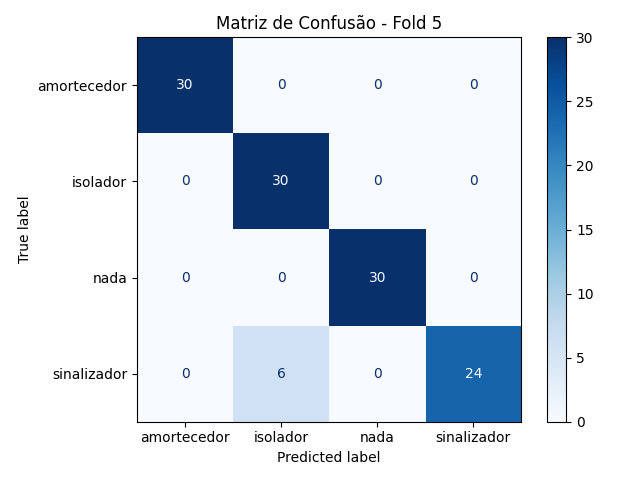
\includegraphics[width=0.7\linewidth]{figuras/Resultados/simu_principal_Teste2_knn.png}
\fonte{}
\label{fig:matriz_confusao_knn_lidar_bruto}
\end{figure}

\paragraph{Árvore de Decisão}

\begin{table}[H]
\centering
\caption{Desempenho da Árvore de Decisão com dados brutos do LiDAR (simulação)}
\label{tab:arvore_lidar_sim}
\begin{tabular}{ccccc}
\hline
\textbf{Dobra} & \textbf{Época Final} & \textbf{Perda Final} & \textbf{Acurácia (\%)} & \textbf{Tempo de Validação (s)} \\
\hline
1 & -  & -      & 100.00 & 0.0001 \\
2 & -  & -      & 99.17  & 0.0001 \\
3 & -  & -      & 99.17  & 0.0002 \\
4 & -  & -      & 100.00 & 0.0002 \\
5 & -  & -      & 99.17  & 0.0001 \\
\hline
\textbf{Média} & - & - & 99.50 & 0.0001 \\
\hline
\end{tabular} \fonte{}
\end{table}

\begin{figure}[H]
\caption{Árvore de decisão gerada para a dobra 1 utilizando dados brutos do LiDAR (simulação).}
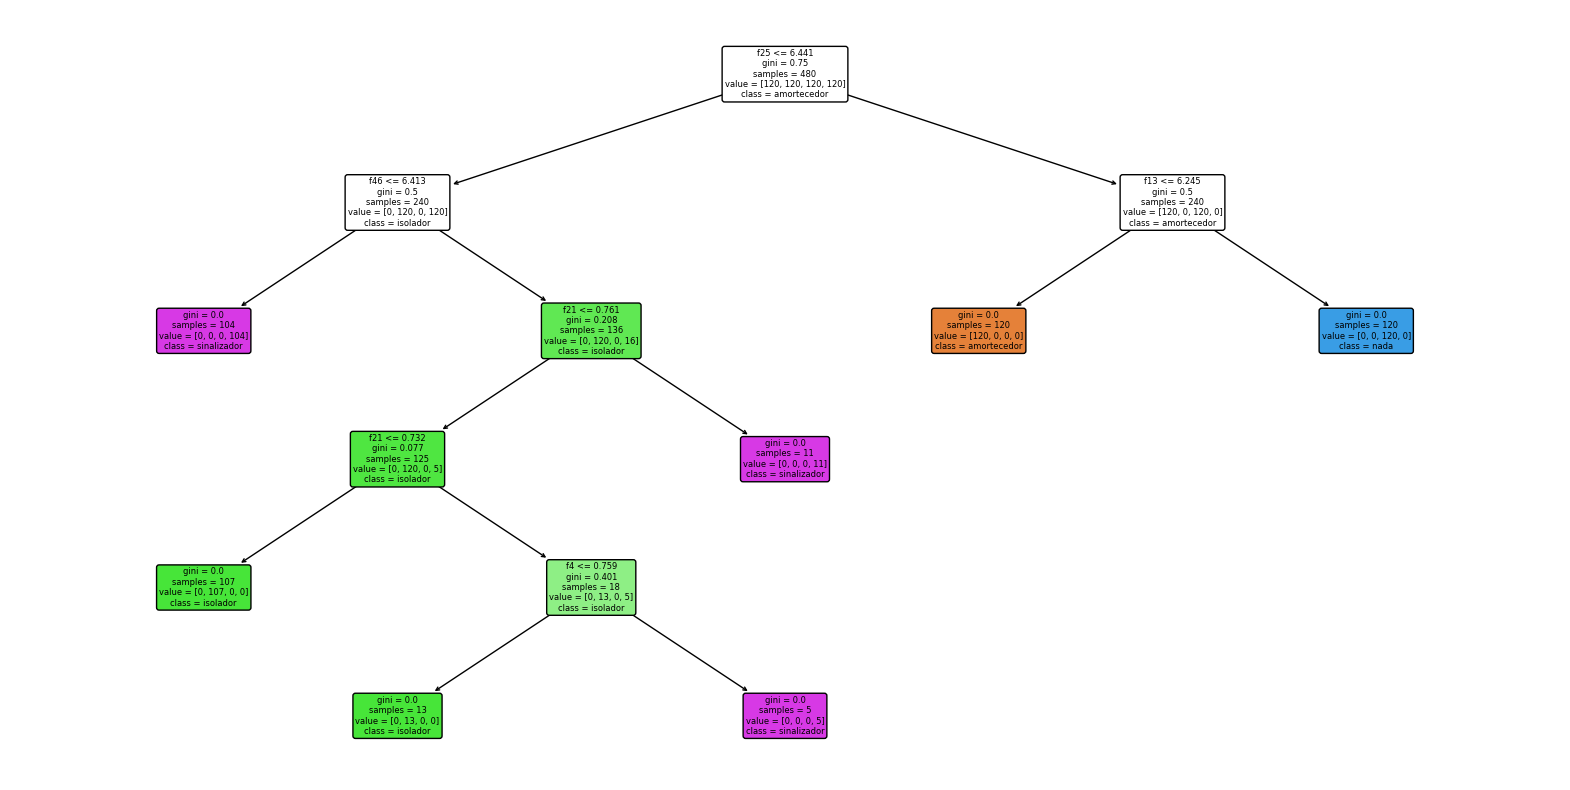
\includegraphics[width=0.9\textwidth]{figuras/Resultados/simu_principal_Teste2_arvore.png}
\fonte{}
\label{fig:arvore_decisao_dobra1}
\end{figure}


\paragraph{Naive Bayes}

\begin{table}[H]
\centering
\caption{Desempenho do Naive Bayes com dados brutos do LiDAR (simulação)}
\label{tab:naive_lidar_bruto}
\begin{tabular}{ccccc}
\hline
\textbf{Dobra} & \textbf{Época Final} & \textbf{Perda Final} & \textbf{Acurácia (\%)} & \textbf{Tempo de Validação (s)} \\
\hline
1 & - & --      & 99.17 & 0.0003 \\
2 & - & --      & 97.50 & 0.0005 \\
3 & - & --      & 97.50 & 0.0003 \\
4 & - & --      & 97.50 & 0.0003 \\
5 & - & --      & 93.33 & 0.0003 \\
\hline
\textbf{Média} & - & -- & 96.60 & 0.0003 \\
\hline
\end{tabular} \fonte{}
\end{table}

\begin{figure}[H]
\caption{Matriz de confusão do Naive Bayes na dobra 5 com dados brutos do LiDAR (simulação).}
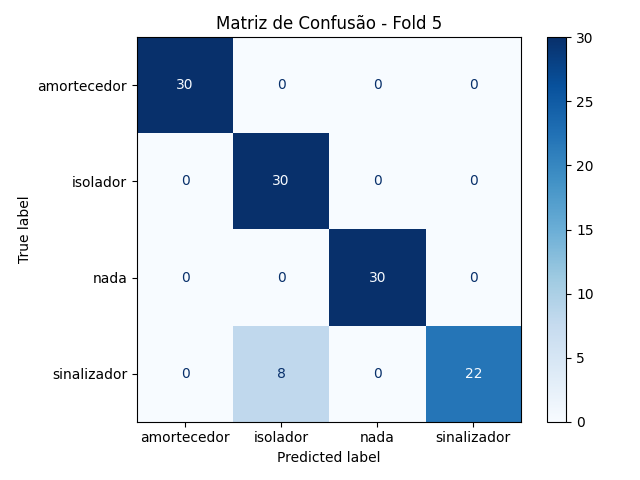
\includegraphics[width=0.7\linewidth]{figuras/Resultados/simu_principal_Teste2_naive.png}
\fonte{}
\label{fig:matriz_confusao_naive_lidar_bruto}
\end{figure}


\paragraph{Rede Neural}

\begin{table}[H]
\centering
\caption{Desempenho da Rede Neural com dados brutos do LiDAR (simulação)}
\label{tab:rede_neural_lidar_bruto}
\begin{tabular}{ccccc}
\hline
\textbf{Dobra} & \textbf{Época Final} & \textbf{Perda Final} & \textbf{Acurácia (\%)} & \textbf{Tempo de Validação (s)} \\
\hline
1 & 200 & 0.033461 & 96.67 & 0.0094 \\
2 & 200 & 0.025889 & 95.83 & 0.0021 \\
3 & 200 & 0.029690 & 98.33 & 0.0019 \\
4 & 200 & 0.029371 & 97.50 & 0.0019 \\
5 & 200 & 0.031941 & 93.33 & 0.0022 \\
\hline
\textbf{Média} & 200.0 & 0.030070 & 96.73 & 0.0035 \\
\hline
\end{tabular} \fonte{}
\end{table}

\begin{figure}[H]
\caption{Matriz de confusão da Rede Neural na dobra 2 com dados brutos do LiDAR (simulação).}
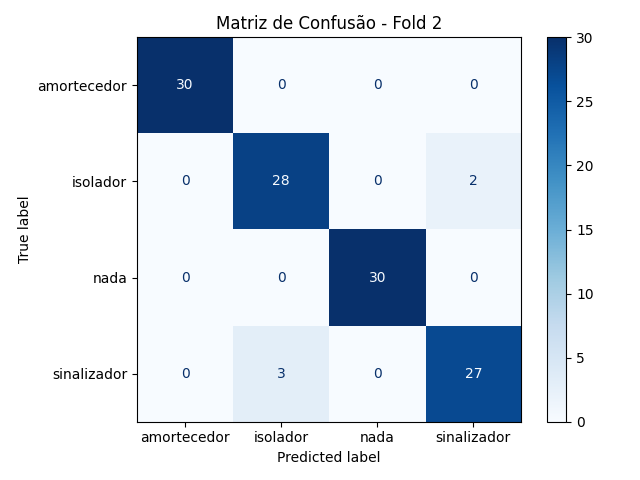
\includegraphics[width=0.7\linewidth]{figuras/Resultados/simu_principal_Teste2_nn.png}
\fonte{}
\label{fig:matriz_confusao_nn_lidar_bruto}
\end{figure}


\paragraph{Floresta Aleatória}

\begin{table}[!h]
\centering
\caption{Desempenho da Floresta Aleatória com dados brutos do LiDAR (simulação)}
\label{tab:rede_neural_features_imagem}
\begin{tabular}{ccccc}
\hline
\textbf{Dobra} & \textbf{Época Final} & \textbf{Perda Final} & \textbf{Acurácia (\%)} & \textbf{Tempo de Validação (s)} \\
\hline
1 & - & - & 100.0  & 0.0061 \\
2 & - & - & 99.17  & 0.0061 \\
3 & - & - & 99.17  & 0.0059 \\
4 & - & - & 100.0  & 0.0059 \\
5 & - & - & 100.0  & 0.0062 \\
\hline
\textbf{Média} & - & - & 99.7 & 0.0060 \\
\hline
\end{tabular} \fonte{}
\end{table}

\subsubsection{Features extraídas das imagens}

Esta subseção apresenta os resultados obtidos com o uso de \textit{features} extraídas das imagens de profundidade simuladas no robô principal. As imagens foram previamente processadas para extração de características numéricas representativas.

\paragraph{k-Vizinhos mais próximos}

\begin{table}[H]
\centering
\caption{Desempenho do k-Vizinhos mais próximos com features extraídas das imagens (simulação)}
\label{tab:knn_feat_img_simu}
\begin{tabular}{ccccc}
\hline
\textbf{Dobra} & \textbf{Época Final} & \textbf{Perda Final} & \textbf{Acurácia (\%)} & \textbf{Tempo de Validação (s)} \\
\hline
1 & - & - & 100.0 & 0.0029 \\
2 & - & - & 100.0 & 0.0054 \\
3 & - & - & 100.0 & 0.0027 \\
4 & - & - & 100.0 & 0.0028 \\
5 & - & - & 100.0 & 0.0028 \\
\hline
\textbf{Média} & - & - & 100.0 & 0.0033 \\
\hline
\end{tabular} \fonte{}
\end{table}

\paragraph{Árvore de Decisão}

\begin{table}[H]
\centering
\caption{Desempenho da Árvore de Decisão com features extraídas das imagens (simulação)}
\label{tab:tree_feat_img_simu}
\begin{tabular}{ccccc}
\hline
\textbf{Dobra} & \textbf{Época Final} & \textbf{Perda Final} & \textbf{Acurácia (\%)} & \textbf{Tempo de Validação (s)} \\
\hline
1 & - & - & 100.0 & 0.000138 \\
2 & - & - & 100.0 & 0.000123 \\
3 & - & - & 100.0 & 0.000124 \\
4 & - & - & 100.0 & 0.000124 \\
5 & - & - & 100.0 & 0.000124 \\
\hline
\textbf{Média} & - & - & 100.0 & 0.000127 \\
\hline
\end{tabular} \fonte{}
\end{table}

\paragraph{Naive Bayes}

\begin{table}[H]
\centering
\caption{Desempenho do Naive Bayes com features extraídas das imagens (simulação)}
\label{tab:naive_feat_img_simu}
\begin{tabular}{ccccc}
\hline
\textbf{Dobra} & \textbf{Época Final} & \textbf{Perda Final} & \textbf{Acurácia (\%)} & \textbf{Tempo de Validação (s)} \\
\hline
1 & - & - & 100.0 & 0.000209 \\
2 & - & - & 99.17 & 0.000212 \\
3 & - & - & 100.0 & 0.000194 \\
4 & - & - & 100.0 & 0.000211 \\
5 & - & - & 100.0 & 0.000214 \\
\hline
\textbf{Média} & - & - & 99.83 & 0.000208 \\
\hline
\end{tabular} \fonte{}
\end{table} 

\paragraph{Rede Neural}

\begin{table}[H]
\centering
\caption{Desempenho da Rede Neural com features extraídas das imagens (simulação)}
\label{tab:nn_feat_img_simu}
\begin{tabular}{ccccc}
\hline
\textbf{Dobra} & \textbf{Época Final} & \textbf{Perda Final} & \textbf{Acurácia (\%)} & \textbf{Tempo de Validação (s)} \\
\hline
1 & 79 & 0.000395 & 100.0 & 0.0117 \\
2 & 34 & 0.000362 & 100.0 & 0.0021 \\
3 & 63 & 0.000620 & 100.0 & 0.0024 \\
4 & 74 & 0.000415 & 99.17 & 0.0021 \\
5 & 49 & 0.000421 & 100.0 & 0.0025 \\
\hline
\textbf{Média} & 59.8 & 0.000443 & 99.83 & 0.0042 \\
\hline
\end{tabular} \fonte{}
\end{table}

\paragraph{Floresta Aleatória}

\begin{table}[H]
\centering
\caption{Desempenho da Floresta Aleatória com features extraídas das imagens (simulação)}
\label{tab:rf_feat_img_simu}
\begin{tabular}{ccccc}
\hline
\textbf{Dobra} & \textbf{Época Final} & \textbf{Perda Final} & \textbf{Acurácia (\%)} & \textbf{Tempo de Validação (s)} \\
\hline
1 & - & - & 100.0 & 0.0055 \\
2 & - & - & 100.0 & 0.0055 \\
3 & - & - & 100.0 & 0.0053 \\
4 & - & - & 100.0 & 0.0052 \\
5 & - & - & 100.0 & 0.0052 \\
\hline
\textbf{Média} & - & - & 100.0 & 0.0054 \\
\hline
\end{tabular} \fonte{}
\end{table}

\subsubsection{Features extraídas do LiDAR}

Esta subseção apresenta os resultados obtidos a partir de atributos derivados dos dados brutos de distância do sensor \textit{LiDAR}, coletados em simulações com o robô principal. As leituras foram processadas para extrair informações relevantes (\textit{features}) que pudessem melhorar a capacidade dos modelos de aprendizado de máquina.

\paragraph{k-Vizinhos mais próximos}

\begin{table}[H]
\centering
\caption{Desempenho do k-Vizinhos mais próximos com features extraídas do LiDAR (simulação)}
\label{tab:knn_features_lidar_simulado}
\begin{tabular}{ccccc}
\hline
\textbf{Dobra} & \textbf{Época Final} & \textbf{Perda Final} & \textbf{Acurácia (\%)} & \textbf{Tempo de Validação (s)} \\
\hline
1 & - & - & 97.5  & 0.0027 \\
2 & - & - & 95.0  & 0.0026 \\
3 & - & - & 96.67 & 0.0030 \\
4 & - & - & 96.67 & 0.0029 \\
5 & - & - & 93.33 & 0.0028 \\
\hline
\textbf{Média} & - & - & 95.83 & 0.0028 \\
\hline
\end{tabular} \fonte{}
\end{table}

\begin{figure}[H]
\caption{Matriz de confusão do k-Vizinhos mais próximos na dobra 5 com features extraídas do LiDAR (simulação).}
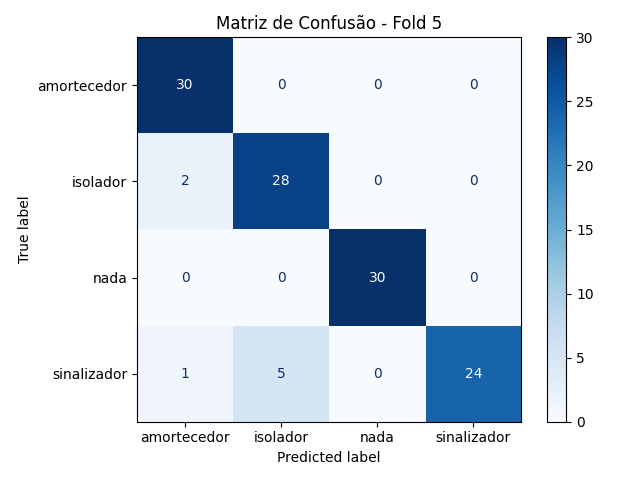
\includegraphics[width=0.7\linewidth]{figuras/Resultados/simu_principal_Teste4_knn.png}
\fonte{}
\label{fig:matriz_confusao_knn_lidar_features}
\end{figure}


\paragraph{Árvore de Decisão}

\begin{table}[H]
\centering
\caption{Desempenho da Árvore de Decisão com features extraídas do LiDAR (simulação)}
\label{tab:arvore_features_lidar_simulado}
\begin{tabular}{ccccc}
\hline
\textbf{Dobra} & \textbf{Época Final} & \textbf{Perda Final} & \textbf{Acurácia (\%)} & \textbf{Tempo de Validação (s)} \\
\hline
1 & - & - & 98.33 & 0.0001 \\
2 & - & - & 98.33 & 0.0002 \\
3 & - & - & 99.17 & 0.0001 \\
4 & - & - & 98.33 & 0.0001 \\
5 & - & - & 96.67 & 0.0002 \\
\hline
\textbf{Média} & - & - & 98.17 & 0.0001 \\
\hline
\end{tabular} \fonte{}
\end{table}

\paragraph{Naive Bayes}

\begin{table}[H]
\centering
\caption{Desempenho do Naive Bayes com features extraídas do LiDAR (simulação)}
\label{tab:naive_features_lidar_simulado}
\begin{tabular}{ccccc}
\hline
\textbf{Dobra} & \textbf{Época Final} & \textbf{Perda Final} & \textbf{Acurácia (\%)} & \textbf{Tempo de Validação (s)} \\
\hline
1 & - & - & 94.17 & 0.00022 \\
2 & - & - & 95.00 & 0.00021 \\
3 & - & - & 94.17 & 0.00034 \\
4 & - & - & 95.00 & 0.00033 \\
5 & - & - & 90.00 & 0.00020 \\
\hline
\textbf{Média} & - & - & 93.67 & 0.00026 \\
\hline
\end{tabular} \fonte{}
\end{table}

\begin{figure}[H]
\caption{Matriz de confusão do Naive Bayes na dobra 5 com features extraídas do LiDAR (simulação).}
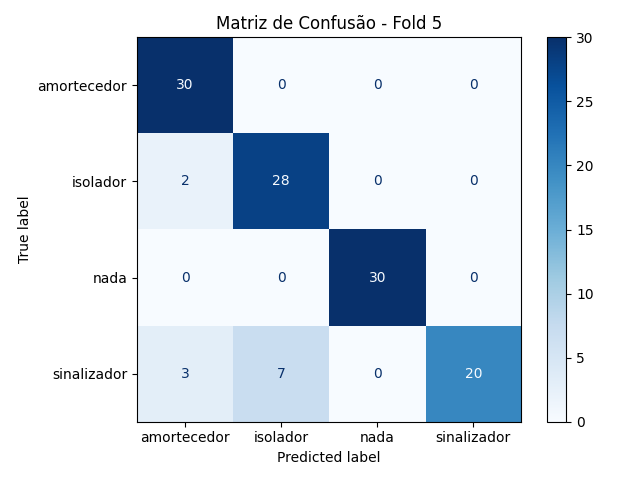
\includegraphics[width=0.7\linewidth]{figuras/Resultados/simu_principal_Teste4_naive.png}
\fonte{}
\label{fig:matriz_confusao_naive_lidar_features}
\end{figure}

\paragraph{Rede Neural}

\begin{table}[H]
\centering
\caption{Desempenho da Rede Neural com features extraídas do LiDAR (simulação)}
\label{tab:rede_neural_lidar_features}
\begin{tabular}{ccccc}
\hline
\textbf{Dobra} & \textbf{Época Final} & \textbf{Perda Final} & \textbf{Acurácia (\%)} & \textbf{Tempo de Validação (s)} \\
\hline
1 & 200 & 0.214619 & 95.00 & 0.00914 \\
2 & 200 & 0.203636 & 94.17 & 0.00183 \\
3 & 200 & 0.202239 & 93.33 & 0.00210 \\
4 & 200 & 0.223546 & 95.83 & 0.00187 \\
5 & 200 & 0.213401 & 89.17 & 0.00193 \\
\hline
\textbf{Média} & 200 & 0.211088 & 93.90 & 0.00377 \\
\hline
\end{tabular}
\fonte{}
\end{table}

\begin{figure}[H]
\caption{Matriz de confusão da Rede Neural na dobra 5 com features extraídas do LiDAR (simulação).}
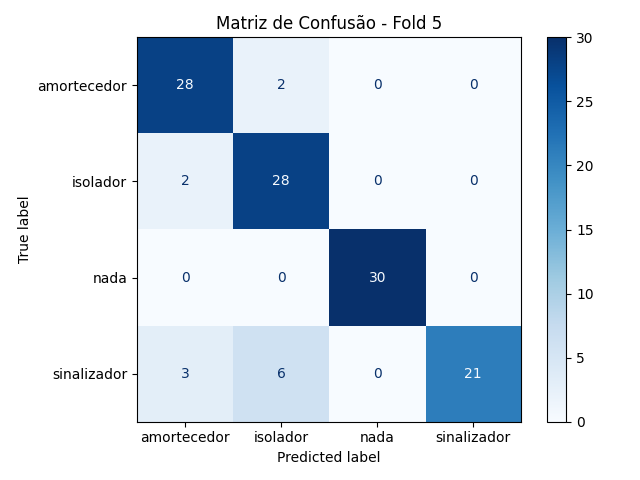
\includegraphics[width=0.7\linewidth]{figuras/Resultados/simu_principal_Teste4_nn.png}
\fonte{}
\label{fig:matriz_confusao_nn_lidar_features}
\end{figure}


\paragraph{Floresta Aleatória}

\begin{table}[H]
\centering
\caption{Desempenho da Floresta Aleatória com features extraídas do LiDAR (simulação)}
\label{tab:floresta_aleatoria_lidar_features}
\begin{tabular}{ccccc}
\hline
\textbf{Dobra} & \textbf{Época Final} & \textbf{Perda Final} & \textbf{Acurácia (\%)} & \textbf{Tempo de Validação (s)} \\
\hline
1 & -   & -        & 98.33 & 0.00586 \\
2 & -   & -        & 95.00 & 0.00551 \\
3 & -   & -        & 98.33 & 0.00582 \\
4 & -   & -        & 98.33 & 0.00550 \\
5 & -   & -        & 97.50 & 0.00572 \\
\hline
\textbf{Média} & - & - & 97.50 & 0.00566 \\
\hline
\end{tabular}
\fonte{}
\end{table}

\subsubsection{Features combinadas}

Esta subseção apresenta os resultados obtidos a partir da combinação das \textit{features} extraídas das imagens e dos dados do sensor \textit{LiDAR}, coletados em simulações com o robô principal.

\paragraph{k-Vizinhos mais próximos}

\begin{table}[H]
\centering
\caption{Desempenho do k-Vizinhos mais próximos com features combinadas (simulação)}
\label{tab:knn_features_combinadas}
\begin{tabular}{ccccc}
\hline
\textbf{Dobra} & \textbf{Época Final} & \textbf{Perda Final} & \textbf{Acurácia (\%)} & \textbf{Tempo de Validação (s)} \\
\hline
1 & - & -       & 100.0 & 0.0027 \\
2 & - & -       & 100.0 & 0.0028 \\
3 & - & -       & 100.0 & 0.0029 \\
4 & - & -       & 100.0 & 0.0027 \\
5 & - & -       & 100.0 & 0.0030 \\
\hline
\textbf{Média} & 1 & -      & 100.0 & 0.00282 \\
\hline
\end{tabular}
\fonte{}
\end{table}

\paragraph{Árvore de Decisão}

\begin{table}[H]
\centering
\caption{Desempenho da Árvore de Decisão com features combinadas (simulação)}
\label{tab:arvore_features_combinadas}
\begin{tabular}{ccccc}
\hline
\textbf{Dobra} & \textbf{Época Final} & \textbf{Perda Final} & \textbf{Acurácia (\%)} & \textbf{Tempo de Validação (s)} \\
\hline
1 & - & -       & 100.0 & 0.000137 \\
2 & - & -       & 100.0 & 0.000128 \\
3 & - & -       & 100.0 & 0.000121 \\
4 & - & -       & 100.0 & 0.000174 \\
5 & - & -       & 100.0 & 0.000122 \\
\hline
\textbf{Média} & 1 & -      & 100.0 & 0.000136 \\
\hline
\end{tabular}
\fonte{}
\end{table}

\paragraph{Naive Bayes}

\begin{table}[H]
\centering
\caption{Desempenho do Naive Bayes com features combinadas (simulação)}
\label{tab:naive_bayes_features_combinadas}
\begin{tabular}{ccccc}
\hline
\textbf{Dobra} & \textbf{Época Final} & \textbf{Perda Final} & \textbf{Acurácia (\%)} & \textbf{Tempo de Validação (s)} \\
\hline
1 & - & -       & 100.0 & 0.000205 \\
2 & - & -       & 99.17 & 0.000200 \\
3 & - & -       & 100.0 & 0.000215 \\
4 & - & -       & 100.0 & 0.000197 \\
5 & - & -       & 100.0 & 0.000232 \\
\hline
\textbf{Média} & 1 & -      & 99.83 & 0.000210 \\
\hline
\end{tabular}
\fonte{}
\end{table}


\paragraph{Rede Neural}

\begin{table}[H]
\centering
\caption{Desempenho da Rede Neural com features combinadas (simulação)}
\label{tab:rn_features_lidar}
\begin{tabular}{ccccc}
\hline
\textbf{Dobra} & \textbf{Época Final} & \textbf{Perda Final} & \textbf{Acurácia (\%)} & \textbf{Tempo de Validação (s)} \\
\hline
1 & 49  & 0.000374 & 100.0  & 0.0096 \\
2 & 66  & 0.000453 & 99.17  & 0.0022 \\
3 & 98  & 0.000035 & 100.0  & 0.0023 \\
4 & 75  & 0.000934 & 100.0  & 0.0019 \\
5 & 38  & 0.000445 & 100.0  & 0.0020 \\
\hline
\textbf{Média} & 65.2 & 0.000428 & 99.67 & 0.0036 \\
\hline
\end{tabular}
\fonte{}
\end{table}

\paragraph{Floresta Aleatória}

\begin{table}[H]
\centering
\caption{Desempenho da Floresta Aleatória com features combinadas (simulação)}
\label{tab:floresta_features_lidar}
\begin{tabular}{ccccc}
\hline
\textbf{Dobra} & \textbf{Época Final} & \textbf{Perda Final} & \textbf{Acurácia (\%)} & \textbf{Tempo de Validação (s)} \\
\hline
1 & - & - & 100.0 & 0.0057 \\
2 & - & - & 100.0 & 0.0053 \\
3 & - & - & 100.0 & 0.0057 \\
4 & - & - & 100.0 & 0.0058 \\
5 & - & - & 100.0 & 0.0054 \\
\hline
\textbf{Média} & - & - & 100.0 & 0.0056 \\
\hline
\end{tabular}
\fonte{}
\end{table}

\subsection{Dados reais}

Nesta subseção são apresentados os resultados obtidos a partir dos dados reais gerados pelo robô principal durante as execuções no ambiente do laboratório.

\subsubsection{Imagens brutas}

Esta subseção apresenta os resultados obtidos com as imagens de profundidade brutas capturadas pelo robô principal em ambiente real no laboratório.

\begin{table}[H]
\centering
\caption{Desempenho da SqueezeNet com imagens brutas (real)}
\label{tab:squeezenet_lidar_real}
\begin{tabular}{ccccc}
\hline
\textbf{Dobra} & \textbf{Época Final} & \textbf{Perda Final} & \textbf{Acurácia (\%)} & \textbf{Tempo de Validação (s)} \\
\hline
1 & 10 & 0.000032 & 100.0 & 0.7084 \\
2 & 11 & 0.000280 & 100.0 & 0.6005 \\
3 & 9  & 0.000295 & 100.0 & 0.6091 \\
4 & 2  & 0.000004 & 100.0 & 0.6110 \\
5 & 4  & 0.000735 & 100.0 & 0.6307 \\
\hline
\textbf{Média} & 7.2 & 0.000269 & 100.0 & 0.6319 \\
\hline
\end{tabular}
\fonte{}
\end{table}

\subsubsection{Dados brutos do LiDAR}

Esta subseção apresenta os resultados obtidos diretamente dos dados brutos de distância fornecidos pelo sensor \textit{LiDAR}, coletados em ambientes reais com o robô principal. 

\paragraph{k-Vizinhos mais próximos}

\begin{table}[H]
\centering
\caption{Desempenho do k-Vizinhos mais próximos com dados brutos do LiDAR (real)}
\label{tab:knn_lidar_bruto_real_2}
\begin{tabular}{ccccc}
\hline
\textbf{Dobra} & \textbf{Época Final} & \textbf{Perda Final} & \textbf{Acurácia (\%)} & \textbf{Tempo de Validação (s)} \\
\hline
1 & - & - & 87.50 & 0.0039 \\
2 & - & - & 93.33 & 0.0037 \\
3 & - & - & 93.33 & 0.0031 \\
4 & - & - & 91.67 & 0.0032 \\
5 & - & - & 86.67 & 0.0034 \\
\hline
\textbf{Média} & - & - & 90.90 & 0.00346 \\
\hline
\end{tabular}
\fonte{}
\end{table}

\begin{figure}[H]
\caption{Matriz de confusão do k-Vizinhos mais próximos na dobra 1 com dados brutos do LiDAR (real).}
\centering
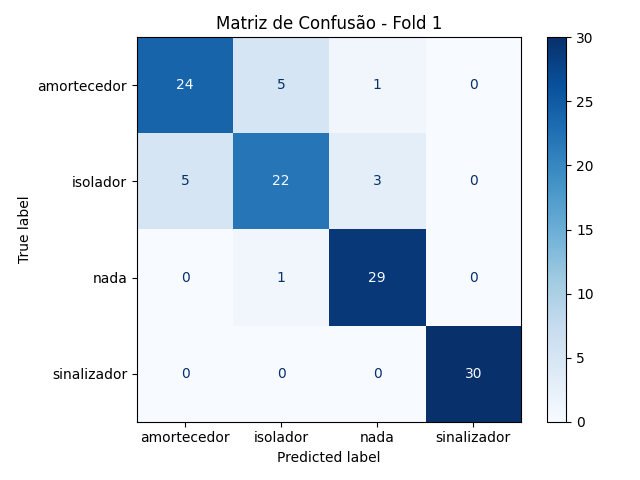
\includegraphics[width=0.7\linewidth]{figuras/Resultados/real_principal_Teste2_knn.png}
\fonte{}
\label{fig:matriz_confusao_knn_lidar_bruto_real}
\end{figure}


\paragraph{Árvore de Decisão}

\begin{table}[H]
\centering
\caption{Desempenho do Árvore de Decisão com dados brutos do LiDAR (real)}
\label{tab:arvore_lidar_bruto_real_2}
\begin{tabular}{ccccc}
\hline
\textbf{Dobra} & \textbf{Época Final} & \textbf{Perda Final} & \textbf{Acurácia (\%)} & \textbf{Tempo de Validação (s)} \\
\hline
1 & - & - & 100.00 & 0.000144 \\
2 & - & - & 99.17 & 0.000139 \\
3 & - & - & 100.00 & 0.000136 \\
4 & - & - & 99.17 & 0.000215 \\
5 & - & - & 97.50 & 0.000159 \\
\hline
\textbf{Média} & - & - & 99.37 & 0.000159 \\
\hline
\end{tabular}
\fonte{}
\end{table}

\paragraph{Naive Bayes}

\begin{table}[H]
\centering
\caption{Desempenho do Naive Bayes com dados brutos do LiDAR (real)}
\label{tab:naive_lidar_bruto_real}
\begin{tabular}{ccccc}
\hline
\textbf{Dobra} & \textbf{Época Final} & \textbf{Perda Final} & \textbf{Acurácia (\%)} & \textbf{Tempo de Validação (s)} \\
\hline
1 & - & - & 86.67 & 0.000273 \\
2 & - & - & 80.83 & 0.000262 \\
3 & - & - & 81.67 & 0.000290 \\
4 & - & - & 80.00 & 0.000286 \\
5 & - & - & 77.50 & 0.000270 \\
\hline
\textbf{Média} & - & - & 81.33 & 0.000276 \\
\hline
\end{tabular}
\fonte{}
\end{table}

\begin{figure}[H]
\caption{Matriz de confusão do Naive Bayes na dobra 2 com dados brutos do LiDAR (real).}
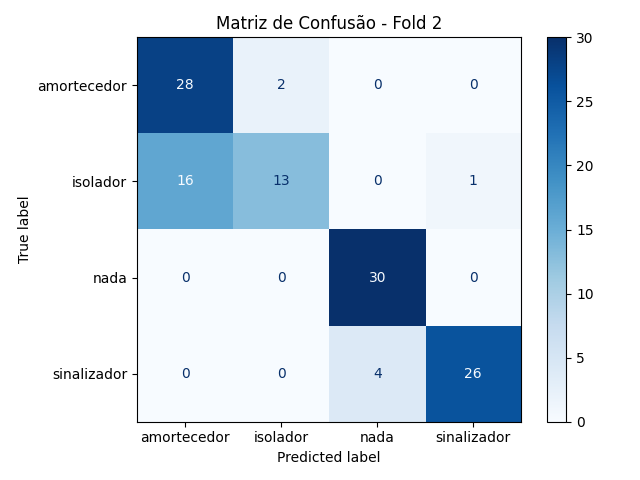
\includegraphics[width=0.7\linewidth]{figuras/Resultados/real_principal_Teste2_naive.png}
\fonte{}
\label{fig:matriz_confusao_naive_lidar_real_dobra2}
\end{figure}

\paragraph{Rede Neural}

\begin{table}[H]
\centering
\caption{Desempenho da Rede Neural com dados brutos do LiDAR (real)}
\label{tab:nn_lidar_bruto_real}
\begin{tabular}{ccccc}
\hline
\textbf{Dobra} & \textbf{Época Final} & \textbf{Perda Final} & \textbf{Acurácia (\%)} & \textbf{Tempo de Validação (s)} \\
\hline
1 & 200 & 0.003282 & 93.33 & 0.010296 \\
2 & 200 & 0.004890 & 94.17 & 0.003278 \\
3 & 200 & 0.004671 & 93.33 & 0.001895 \\
4 & 160 & 0.000999 & 94.17 & 0.001972 \\
5 & 200 & 0.004385 & 90.83 & 0.001836 \\
\hline
\textbf{Média} & 192 & 0.003645 & 93.17 & 0.003855 \\
\hline
\end{tabular}
\fonte{}
\end{table}

\begin{figure}[H]
\caption{Matriz de confusão da Rede Neural na dobra 5 com dados brutos do LiDAR (real).}
\centering
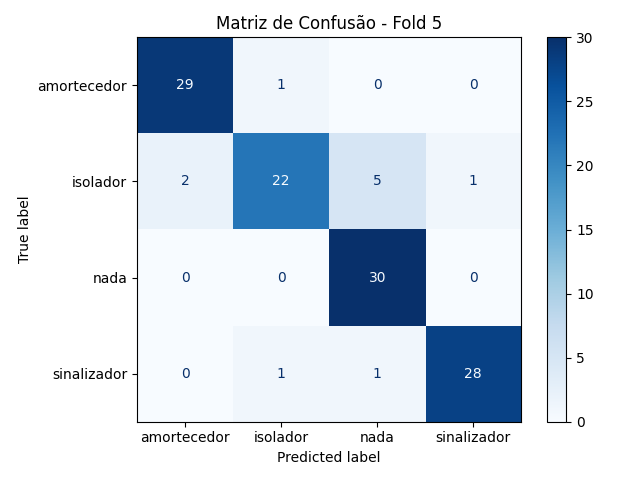
\includegraphics[width=0.7\linewidth]{figuras/Resultados/real_principal_Teste2_nn.png}
\fonte{}
\label{fig:matriz_confusao_nn_lidar_bruto_real}
\end{figure}

\paragraph{Floresta Aleatória}

\begin{table}[H]
\centering
\caption{Desempenho da Floresta Aleatória com dados brutos do LiDAR (real)}
\label{tab:rf_lidar_bruto_real}
\begin{tabular}{ccccc}
\hline
\textbf{Dobra} & \textbf{Época Final} & \textbf{Perda Final} & \textbf{Acurácia (\%)} & \textbf{Tempo de Validação (s)} \\
\hline
1 & - & - & 100.0 & 0.005681 \\
2 & - & - & 100.0 & 0.005755 \\
3 & - & - & 100.0 & 0.005916 \\
4 & - & - & 100.0 & 0.006184 \\
5 & - & - & 100.0 & 0.006251 \\
\hline
\textbf{Média} & - & - & 100.0 & 0.005957 \\
\hline
\end{tabular}
\fonte{}
\end{table}

\subsubsection{Features extraídas das imagens}

Esta subseção apresenta os resultados obtidos a partir de atributos derivados das imagens reais coletadas pelo robô principal. As imagens foram processadas para extrair informações relevantes (\textit{features}) que pudessem melhorar a capacidade dos modelos de aprendizado de máquina na identificação das classes de objetos.

\paragraph{k-Vizinhos mais próximos}

\begin{table}[H]
\caption{Desempenho do k-Vizinhos mais próximos com features extraídas das imagens (real).}
\centering
\begin{tabular}{ccccc}
\hline
\textbf{Dobra} & \textbf{Época Final} & \textbf{Perda Final} & \textbf{Acurácia (\%)} & \textbf{Tempo de Validação (s)}  \\
\hline
1 & - & - & 100,0 & 0,0030 \\
2 & - & - & 100,0 & 0,0030 \\
3 & - & - & 100,0 & 0,0029 \\
4 & - & - & 100,0 & 0,0030 \\
5 & - & - & 100,0 & 0,0031 \\
\hline
\textbf{Média} & - & - & 100,0 & 0,0030 \\
\hline
\end{tabular}
\fonte{}
\label{tab:knn_features_imagens}
\end{table} 

\paragraph{Árvore de Decisão}

\begin{table}[H]
\caption{Desempenho da Árvore de Decisão com features extraídas das imagens (real).}
\centering
\begin{tabular}{ccccc}
\hline
\textbf{Dobra} & \textbf{Época Final} & \textbf{Perda Final} & \textbf{Acurácia (\%)} & \textbf{Tempo de Validação (s)}  \\
\hline
1 & - & - & 100,0 & 0,000154 \\
2 & - & - & 100,0 & 0,000129 \\
3 & - & - & 100,0 & 0,000138 \\
4 & - & - & 100,0 & 0,000135 \\
5 & - & - & 99,17 & 0,000128 \\
\hline
\textbf{Média} & - & - & 99,67 & 0,000137 \\
\hline
\end{tabular}
\fonte{}
\label{tab:arvore_features_imagens}
\end{table}

\paragraph{Naive Bayes}

\begin{table}[H]
\caption{Desempenho do Naive Bayes com features extraídas das imagens (real).}
\centering
\begin{tabular}{ccccc}
\hline
\textbf{Dobra} & \textbf{Época Final} & \textbf{Perda Final} & \textbf{Acurácia (\%)} & \textbf{Tempo de Validação (s)}  \\
\hline
1 & - & - & 99,17 & 0,000196 \\
2 & - & - & 100,0 & 0,000192 \\
3 & - & - & 99,17 & 0,000350 \\
4 & - & - & 100,0 & 0,000243 \\
5 & - & - & 98,33 & 0,000200 \\
\hline
\textbf{Média} & - & - & 99,33 & 0,000236 \\
\hline
\end{tabular}
\fonte{}
\label{tab:naive_features_imagens}
\end{table}


\paragraph{Rede Neural}

\begin{table}[H]
\caption{Desempenho da Rede Neural com features extraídas das imagens (real).}
\centering
\begin{tabular}{ccccc}
\hline
\textbf{Dobra} & \textbf{Época Final} & \textbf{Perda Final} & \textbf{Acurácia (\%)} & \textbf{Tempo de Validação (s)}  \\
\hline
1 & 200 & 7,458555 & 89,17 & 0,009501 \\
2 & 200 & 1,502896 & 87,5 & 0,001873 \\
3 & 200 & 3,814955 & 89,17 & 0,001903 \\
4 & 200 & 10,270095 & 86,67 & 0,001998 \\
5 & 200 & 4,025579 & 86,67 & 0,001852 \\
\hline
\textbf{Média} & 200 & 5,014204 & 87,84 & 0,003025 \\
\hline
\end{tabular}
\fonte{}
\label{tab:rn_features_imagens_real}
\end{table}

\begin{figure}[H]
\caption{Matriz de confusão da Rede Neural na dobra 4 com features extraídas das imagens (real).}
\centering
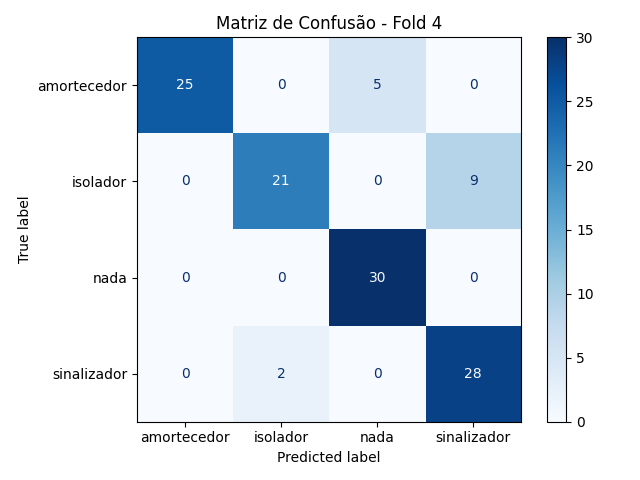
\includegraphics[width=0.7\linewidth]{figuras/Resultados/real_principal_Teste3_nn.png}
\fonte{}
\label{fig:matriz_confusao_rn_imagens_real}
\end{figure}


\paragraph{Floresta Aleatória}

\begin{table}[H]
\caption{Desempenho da Floresta Aleatória com features extraídas das imagens (real).}
\centering
\begin{tabular}{ccccc}
\hline
\textbf{Dobra} & \textbf{Época Final} & \textbf{Perda Final} & \textbf{Acurácia (\%)} & \textbf{Tempo de Validação (s)}  \\
\hline
1 & - & - & 99,17 & 0,005706 \\
2 & - & - & 100,0 & 0,005852 \\
3 & - & - & 100,0 & 0,005603 \\
4 & - & - & 100,0 & 0,005454 \\
5 & - & - & 100,0 & 0,005498 \\
\hline
\textbf{Média} & - & - & 99,67 & 0,005623 \\
\hline
\end{tabular}
\fonte{}
\label{tab:rf_features_imagens_real}
\end{table}


\subsubsection{Features extraídas do LiDAR}

Esta subseção apresenta os resultados obtidos a partir de atributos derivados dos dados brutos reais de distância do sensor \textit{LiDAR}, coletados com o robô principal. As leituras foram processadas para extrair informações relevantes (\textit{features}) que pudessem melhorar a capacidade dos modelos de aprendizado de máquina.

\paragraph{k-Vizinhos mais próximos}

\begin{table}[H]
\caption{Desempenho do k-Vizinhos mais próximos com features extraídas do LiDAR (real).}
\centering
\begin{tabular}{ccccc}
\hline
\textbf{Dobra} & \textbf{Época Final} & \textbf{Perda Final} & \textbf{Acurácia (\%)} & \textbf{Tempo de Validação (s)}  \\
\hline
1 & - & - & 91,67 & 0,0030 \\
2 & - & - & 94,17 & 0,0027 \\
3 & - & - & 94,17 & 0,0028 \\
4 & - & - & 95,83 & 0,0028 \\
5 & - & - & 90,00 & 0,0027 \\
\hline
\textbf{Média} & - & - & 93,17 & 0,0028 \\
\hline
\end{tabular}
\fonte{}
\label{tab:knn_features_imagens_real}
\end{table}

\begin{figure}[H]
\caption{Matriz de confusão do k-Vizinhos mais próximos na dobra 5 com features extraídas do LiDAR (real).}
\centering
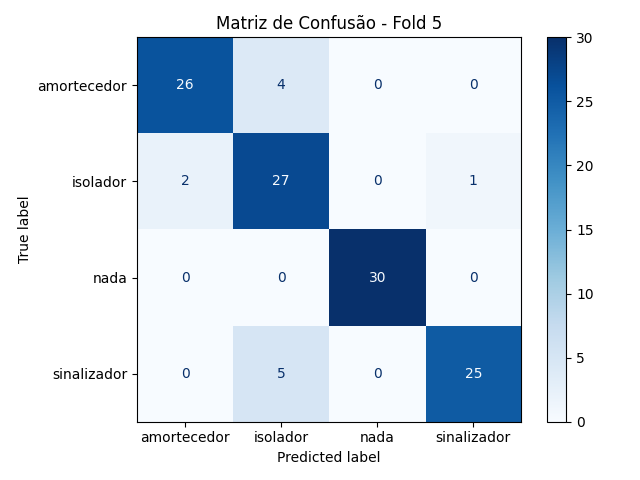
\includegraphics[width=0.7\linewidth]{figuras/Resultados/real_principal_Teste4_knn.png}
\fonte{}
\label{fig:matriz_confusao_knn_imagens_real_dobra5}
\end{figure}

\paragraph{Árvore de Decisão}

\begin{table}[H]
\caption{Desempenho da Árvore de Decisão com features extraídas do LiDAR (real).}
\centering
\begin{tabular}{ccccc}
\hline
\textbf{Dobra} & \textbf{Época Final} & \textbf{Perda Final} & \textbf{Acurácia (\%)} & \textbf{Tempo de Validação (s)}  \\
\hline
1 & - & - & 97,50 & 0,000133 \\
2 & - & - & 99,17 & 0,000135 \\
3 & - & - & 97,50 & 0,000124 \\
4 & - & - & 98,33 & 0,000137 \\
5 & - & - & 95,00 & 0,000138 \\
\hline
\textbf{Média} & - & - & 97,50 & 0,000134 \\
\hline
\end{tabular}
\fonte{}
\label{tab:arvore_decisao_features_imagens_real}
\end{table}

\paragraph{Naive Bayes}

\begin{table}[H]
\caption{Desempenho do Naive Bayes com features extraídas do LiDAR (real).}
\centering
\begin{tabular}{ccccc}
\hline
\textbf{Dobra} & \textbf{Época Final} & \textbf{Perda Final} & \textbf{Acurácia (\%)} & \textbf{Tempo de Validação (s)}  \\
\hline
1 & - & - & 96,67 & 0,00026 \\
2 & - & - & 94,17 & 0,000252 \\
3 & - & - & 93,33 & 0,000207 \\
4 & - & - & 93,33 & 0,000205 \\
5 & - & - & 90,00 & 0,000295 \\
\hline
\textbf{Média} & - & - & 93,90 & 0,000244 \\
\hline
\end{tabular}
\fonte{}
\label{tab:naive_bayes_features_imagens_real}
\end{table}

\begin{figure}[H]
\caption{Matriz de confusão do Naive Bayes na dobra 5 com features extraídas do LiDAR (real).}
\centering
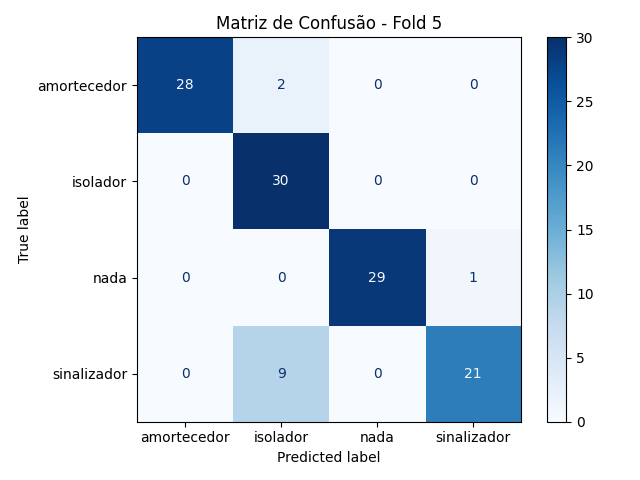
\includegraphics[width=0.7\linewidth]{figuras/Resultados/real_principal_Teste4_naive.png}
\fonte{}
\label{fig:matriz_confusao_naive_imagens_real}
\end{figure}

\paragraph{Rede Neural}

\begin{table}[H]
\caption{Desempenho da Rede Neural com features extraídas do LiDAR (real).}
\centering
\begin{tabular}{ccccc}
\hline
\textbf{Dobra} & \textbf{Época Final} & \textbf{Perda Final} & \textbf{Acurácia (\%)} & \textbf{Tempo de Validação (s)}  \\
\hline
1 & 200 & 0.135437 & 96.67 & 0.010137 \\
2 & 200 & 0.121473 & 95.83 & 0.002069 \\
3 & 200 & 0.143646 & 95.83 & 0.002144 \\
4 & 200 & 0.109989 & 96.67 & 0.002189 \\
5 & 200 & 0.168874 & 90.00 & 0.001935 \\
\hline
\multicolumn{3}{c}{Média} & 95.00 & 0.003295 \\
\hline
\end{tabular}
\fonte{}
\label{tab:resultados_nn_imagens_real}
\end{table}

\begin{figure}[H]
\caption{Matriz de confusão da Rede Neural na dobra 5 com features extraídas do LiDAR (real).}
\centering
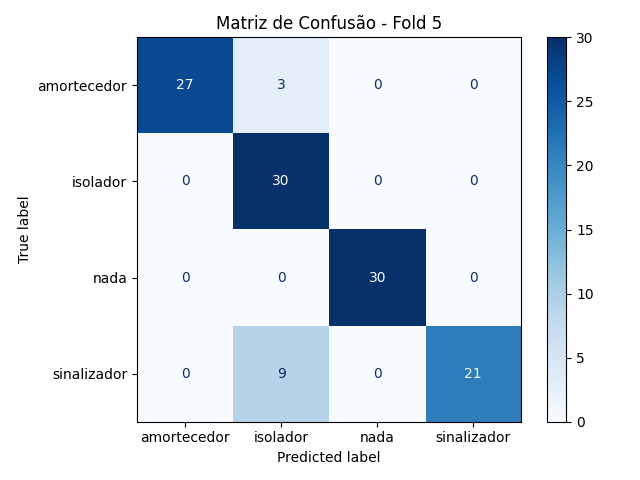
\includegraphics[width=0.7\linewidth]{figuras/Resultados/real_principal_Teste4_nn.png}
\fonte{}
\label{fig:matriz_confusao_nn_imagens_real}
\end{figure}


\paragraph{Floresta Aleatória}

\begin{table}[H]
\caption{Desempenho da Floresta Aleatória com features extraídas do LiDAR (real).}
\centering
\begin{tabular}{ccccc}
\hline
\textbf{Dobra} & \textbf{Época Final} & \textbf{Perda Final} & \textbf{Acurácia (\%)} & \textbf{Tempo de Validação (s)}  \\
\hline
1 & - & - & 100.0 & 0.005577 \\
2 & - & - & 98.33 & 0.005834 \\
3 & - & - & 99.17 & 0.006009 \\
4 & - & - & 96.67 & 0.005491 \\
5 & - & - & 97.5 & 0.005741 \\
\hline
\multicolumn{3}{c}{Média} & 98.33 & 0.005730 \\
\hline
\end{tabular}
\fonte{}
\label{tab:resultados_rf_imagens_real}
\end{table}


\subsubsection{Features combinadas}

Esta subseção apresenta os resultados obtidos a partir da combinação das \textit{features} extraídas das imagens e dos dados do sensor \textit{LiDAR} reais, coletados com o robô principal.

\paragraph{k-Vizinhos mais próximos}

\begin{table}[H]
\caption{Desempenho do k-Vizinhos mais próximos com features combinadas (real).}
\centering
\begin{tabular}{ccccc}
\hline
\textbf{Dobra} & \textbf{Época Final} & \textbf{Perda Final} & \textbf{Acurácia (\%)} & \textbf{Tempo de Validação (s)}  \\
\hline
1 & - & - & 100.0 & 0.0028 \\
2 & - & - & 100.0 & 0.0028 \\
3 & - & - & 100.0 & 0.0029 \\
4 & - & - & 100.0 & 0.0028 \\
5 & - & - & 100.0 & 0.0031 \\
\hline
\multicolumn{3}{c}{Média} & 100.0 & 0.0029 \\
\hline
\end{tabular}
\fonte{}
\label{tab:resultados_knn_imagens_real}
\end{table}


\paragraph{Árvore de Decisão}

\begin{table}[H]
\caption{Desempenho do Naive Bayes com features combinadas (real).}
\centering
\begin{tabular}{ccccc}
\hline
\textbf{Dobra} & \textbf{Época Final} & \textbf{Perda Final} & \textbf{Acurácia (\%)} & \textbf{Tempo de Validação (s)}  \\
\hline
1 & - & - & 100.0 & 0.000131 \\
2 & - & - & 100.0 & 0.000139 \\
3 & - & - & 100.0 & 0.000138 \\
4 & - & - & 98.33 & 0.000134 \\
5 & - & - & 99.17 & 0.000134 \\
\hline
\multicolumn{3}{c}{Média} & 99.5 & 0.000134 \\
\hline
\end{tabular}
\fonte{}
\label{tab:resultados_naive_imagens_real}
\end{table}

\paragraph{Naive Bayes}

\begin{table}[H]
\caption{Desempenho do Naive Bayes com features combinadas (real).}
\centering
\begin{tabular}{ccccc}
\hline
\textbf{Dobra} & \textbf{Época Final} & \textbf{Perda Final} & \textbf{Acurácia (\%)} & \textbf{Tempo de Validação (s)}  \\
\hline
1 & - & - & 100.0 & 0.000224 \\
2 & - & - & 100.0 & 0.000198 \\
3 & - & - & 100.0 & 0.000210 \\
4 & - & - & 100.0 & 0.000235 \\
5 & - & - & 98.33 & 0.000205 \\
\hline
\multicolumn{3}{c}{Média} & 99.67 & 0.000214 \\
\hline
\end{tabular}
\fonte{}
\label{tab:resultados_naive_lidar_real}
\end{table}

\paragraph{Rede Neural}

\begin{table}[H]
\caption{Desempenho da Rede Neural com features combinadas (real).}
\centering
\begin{tabular}{ccccc}
\hline
\textbf{Dobra} & \textbf{Época Final} & \textbf{Perda Final} & \textbf{Acurácia (\%)} & \textbf{Tempo de Validação (s)}  \\
\hline
1 & 200 & 1.0448 & 94.17 & 0.009344 \\
2 & 200 & 1.9525 & 87.50 & 0.001929 \\
3 & 200 & 3.6604 & 87.50 & 0.001974 \\
4 & 200 & 3.4093 & 95.00 & 0.002141 \\
5 & 200 & 6.8385 & 90.83 & 0.001893 \\
\hline
\multicolumn{3}{c}{Média} & 90.60 & 0.003456 \\
\hline
\end{tabular}
\fonte{}
\label{tab:resultados_nn_lidar_real}
\end{table}

\begin{figure}[H]
\centering
\caption{Matriz de confusão da dobra 3 para a Rede Neural com features combinadas (real).}
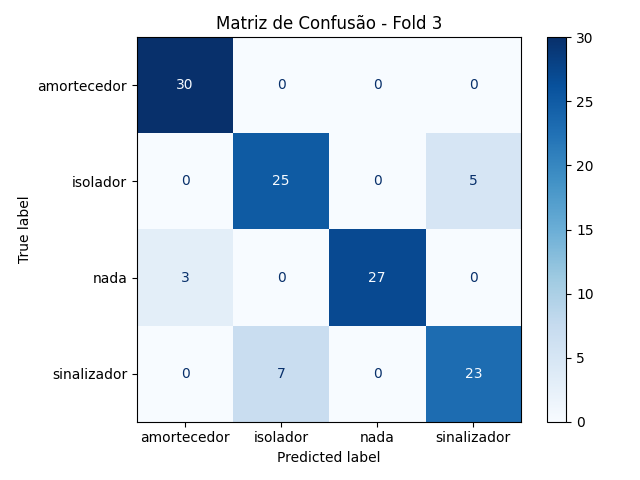
\includegraphics[width=0.7\textwidth]{figuras/Resultados/real_principal_Teste5_nn.png}
\label{fig:matriz_confusao_nn_dobra3}
\fonte{}
\end{figure}


\paragraph{Floresta Aleatória}

\begin{table}[H]
\caption{Desempenho da Floresta Aleatória com features combinadas (real).}
\centering
\begin{tabular}{ccccc}
\hline
\textbf{Dobra} & \textbf{Época Final} & \textbf{Perda Final} & \textbf{Acurácia (\%)} & \textbf{Tempo de Validação (s)}  \\
\hline
1 & - & - & 99.17 & 0.006221 \\
2 & - & - & 100.0 & 0.005471 \\
3 & - & - & 100.0 & 0.005714 \\
4 & - & - & 100.0 & 0.005598 \\
5 & - & - & 100.0 & 0.005813 \\
\hline
\multicolumn{3}{c}{Média} & 99.67 & 0.005763 \\
\hline
\end{tabular}
\fonte{}
\label{tab:resultados_rf_lidar_real}
\end{table}



\section{Resultados com os robôs secundários}

Nesta seção são apresentados os resultados obtidos com os dados provenientes do robôs secundários, utilizados em ambiente simulado. Para ambas topologias analisadas, foi aplicada a validação usando os dados da topologia principal para treinamento e os dados das topologias secundárias para validação, conforme descrito anteriormente. Os resultados estão organizados em subseções separadas, de modo a permitir uma análise clara do desempenho dos modelos em cada tipo de \textit{dataset}. Cada conjunto de dados — imagens brutas, leituras do \textit{LiDAR}, \textit{features} extraídas e combinação de \textit{features} — é avaliado individualmente. As métricas consideradas incluem acurácia média, tempo de validação, perda final e número de épocas, além da matriz de confusão quando relevante. A distinção entre as topologias permite também avaliar a consistência do sensor multimodal frente à variação entre os ambientes.

\subsection{Dados do primeiro robô}

Nesta subseção são apresentados os resultados obtidos a partir dos dados simulados gerados pela primeira topologia secundária em conjunto com os dados do robô principal usados para treinamento.

\subsubsection{Imagens brutas}

Esta subseção apresenta os resultados obtidos com as imagens de profundidade brutas
capturadas pelo primeiro robô das topologias secundárias em ambiente simulado com o modelo treinado pelos dados do robô principal.

\begin{table}[H]
\caption{Desempenho da SqueezeNet com imagens brutas (robô 1 das topologias secundárias).}
\centering
\begin{tabular}{ccccc}
\hline
\textbf{Época Final} & \textbf{Perda Final} & \textbf{Acurácia (\%)} & \textbf{Tempo de Validação (s)}  \\
\hline
3 & 0.00025 & 97.67 & 3.371939 \\
\hline
\end{tabular}
\fonte{}
\label{tab:resultados_nn_topo_secundarias}
\end{table}

\begin{figure}[H]
\centering
\caption{Matriz de confusão do modelo SqueezeNet utilizando imagens brutas (primeiro robô das topologias secundárias).}
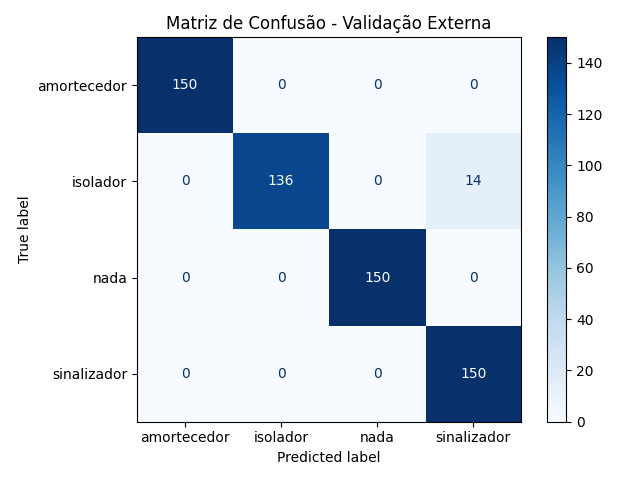
\includegraphics[width=0.7\textwidth]{figuras/Resultados/multi_primeiro_Teste1.png}
\label{fig:mc_squeezenet_imgbrutas_robo1_sim_t1}
\fonte{}
\end{figure}

\subsubsection{Dados brutos do LiDAR}

Esta subseção apresenta os resultados obtidos com os dados brutos do LiDAR capturadas pelo primeiro robô das topologias secundárias em ambiente simulado com o modelo treinado pelos dados do robô principal.

\begin{table}[H]
\caption{Comparativo de desempenho entre diferentes modelos.}
\centering
\begin{tabular}{ccccc}
\hline
\textbf{Modelo} & \textbf{Época Final} & \textbf{Perda Final} & \textbf{Acurácia (\%)} & \textbf{Tempo de Validação (s)}  \\
\hline
kNN      & - & - & 47.83 & 0.01927 \\
Árvore   & - & - & 46.00 & 0.000213 \\ 
Naive    & - & - & 25.00 & 0.000745 \\ 
Rede     & - & - & 25.00 & 0.000745 \\
Floresta & - & - & 46.67 & 0.007682 \\
\hline
\multicolumn{3}{c}{Média} & 38.10 & 0.056262 \\
\hline
\end{tabular}
\fonte{}
\label{tab:comparativo_modelos_atualizado}
\end{table}

\begin{figure}[H]
\centering
\caption{Matriz de confusão para o k-Vizinhos mais próximos com dados brutos do LiDAR (primeiro robô das topologias secundárias).}
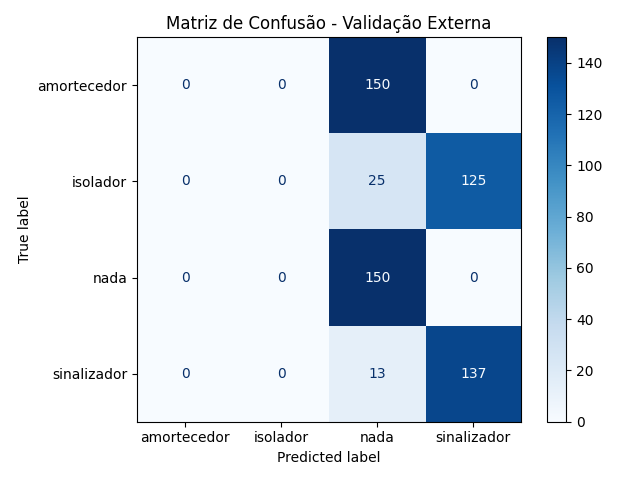
\includegraphics[width=0.7\textwidth]{figuras/Resultados/multi_primeiro_Teste2_knn.png}
\label{fig:mc_lidar_knn_robo1_t2}
\fonte{}
\end{figure}

\begin{figure}[H]
\centering
\caption{Matriz de confusão para a Árvore de Decisão com dados brutos do LiDAR (primeiro robô das topologias secundárias).}
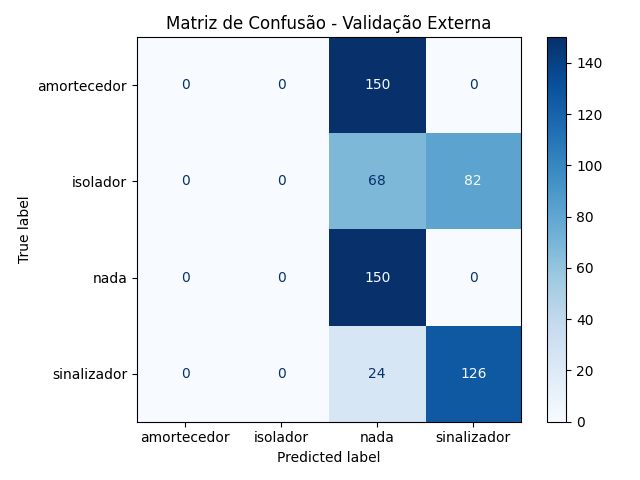
\includegraphics[width=0.7\textwidth]{figuras/Resultados/multi_primeiro_Teste2_tree.png}
\label{fig:mc_lidar_tree_robo1_t2}
\fonte{}
\end{figure}

\begin{figure}[H]
\centering
\caption{Matriz de confusão para o Naive Bayes com dados brutos do LiDAR (primeiro robô das topologias secundárias).}
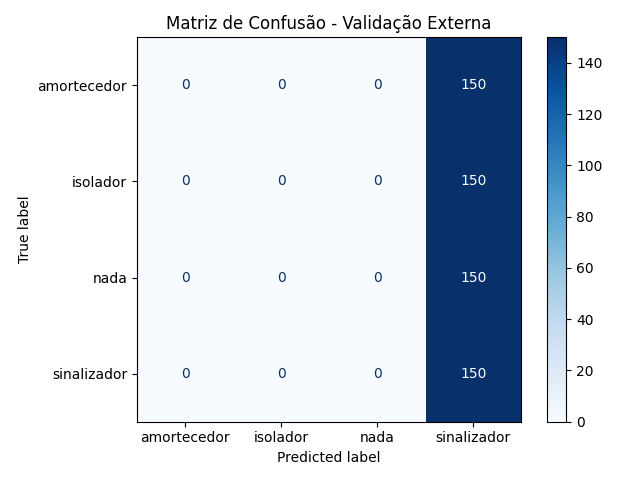
\includegraphics[width=0.7\textwidth]{figuras/Resultados/multi_primeiro_Teste2_naive.png}
\label{fig:mc_lidar_naive_robo1_t2}
\fonte{}
\end{figure}

\begin{figure}[H]
\centering
\caption{Matriz de confusão para a Rede Neural com dados brutos do LiDAR (primeiro robô das topologias secundárias).}
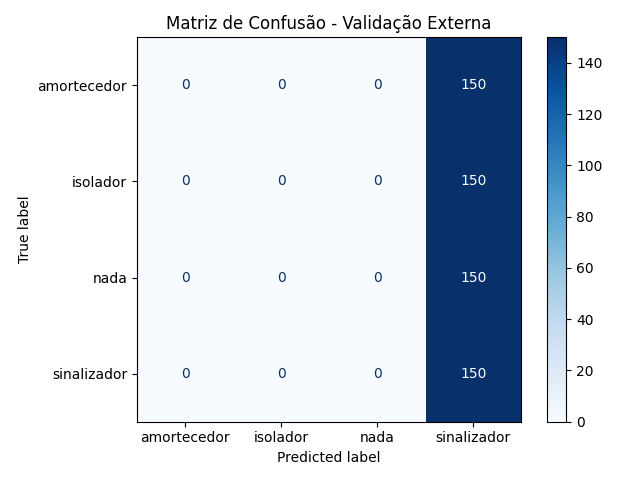
\includegraphics[width=0.7\textwidth]{figuras/Resultados/multi_primeiro_Teste2_nn.png}
\label{fig:mc_lidar_nn_robo1_t2}
\fonte{}
\end{figure}

\begin{figure}[H]
\centering
\caption{Matriz de confusão para a Floresta Aleatória com dados brutos do LiDAR (primeiro robô das topologias secundárias).}
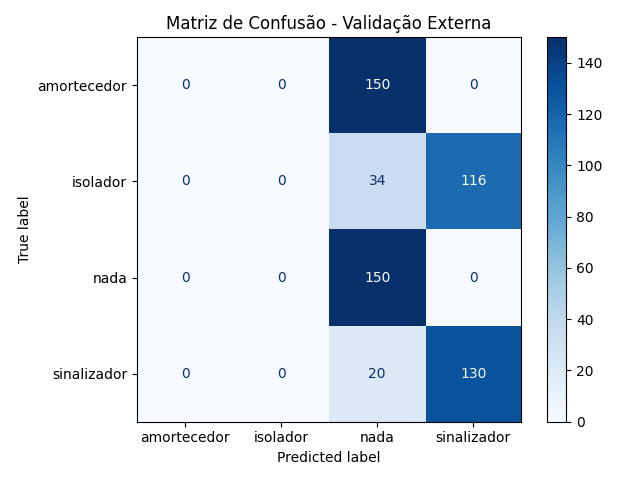
\includegraphics[width=0.7\textwidth]{figuras/Resultados/multi_primeiro_Teste2_rf.png}
\label{fig:mc_lidar_rf_robo1_t2}
\fonte{}
\end{figure}

\subsubsection{Features extraídas das imagens}

Esta subseção apresenta os resultados obtidos a partir de atributos derivados das imagens  capturadas pelo primeiro robô das topologias secundárias em ambiente simulado com o modelo treinado pelos dados do robô principal. As imagens foram processadas para extrair informações relevantes (\textit{features}) que pudessem melhorar a capacidade dos modelos de aprendizado de máquina na identificação das classes de objetos.

\begin{table}[H]
\caption{Desempenho dos modelos com features extraídas das imagens (primeiro robô das topologias secundárias).}
\centering
\begin{tabular}{ccccc}
\hline
\textbf{Modelo} & \textbf{Época Final} & \textbf{Perda Final} & \textbf{Acurácia (\%)} & \textbf{Tempo de Validação (s)}  \\
\hline
kNN      & - & - & 70.33 & 0.012015 \\
Árvore   & - & - & 69.67 & 0.000170 \\
Naive    & - & - & 69.83 & 0.000264 \\
Rede     & 43 & 0.000551 & 75.00 & 0.015986 \\
Floresta & - & - & 69.67 & 0.007539 \\
\hline
\multicolumn{3}{c}{Média} & 70.90 & 0.007195 \\
\hline
\end{tabular}
\fonte{}
\label{tab:modelos_feat_imagens_robo1}
\end{table}


\begin{figure}[H]
\centering
\caption{Matriz de confusão para o k-Vizinhos mais próximos com features extraídas das imagens (primeiro robô das topologias secundárias).}
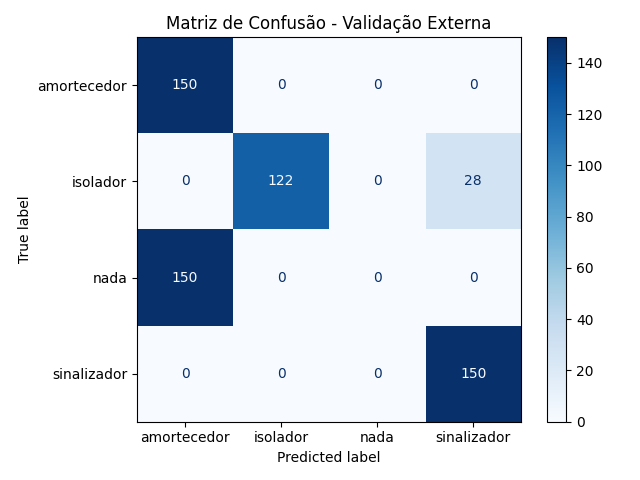
\includegraphics[width=0.7\textwidth]{figuras/Resultados/multi_primeiro_Teste3_knn.png}
\label{fig:mc_featimg_knn_robo1_t3}
\fonte{}
\end{figure}

\begin{figure}[H]
\centering
\caption{Matriz de confusão para a Árvore de Decisão com features extraídas das imagens (primeiro robô das topologias secundárias).}
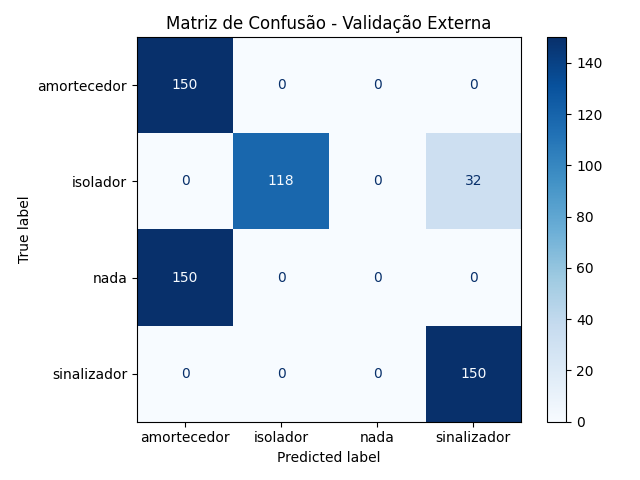
\includegraphics[width=0.7\textwidth]{figuras/Resultados/multi_primeiro_Teste3_tree.png}
\label{fig:mc_featimg_tree_robo1_t3}
\fonte{}
\end{figure}

\begin{figure}[H]
\centering
\caption{Matriz de confusão para o Naive Bayes com features extraídas das imagens (primeiro robô das topologias secundárias).}
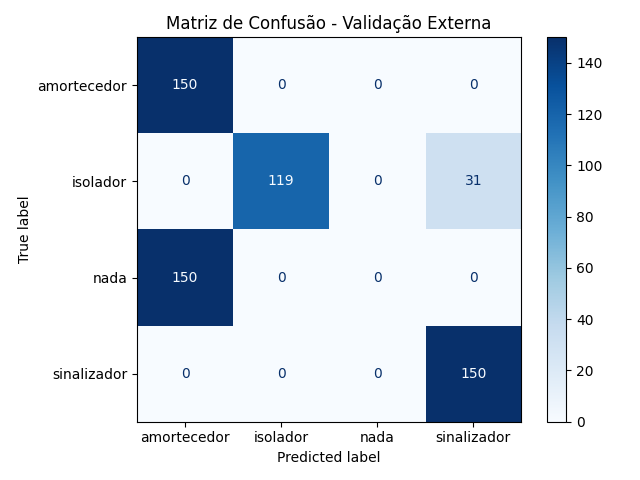
\includegraphics[width=0.7\textwidth]{figuras/Resultados/multi_primeiro_Teste3_naive.png}
\label{fig:mc_featimg_naive_robo1_t3}
\fonte{}
\end{figure}

\begin{figure}[H]
\centering
\caption{Matriz de confusão para a Rede Neural com features extraídas das imagens (primeiro robô das topologias secundárias).}
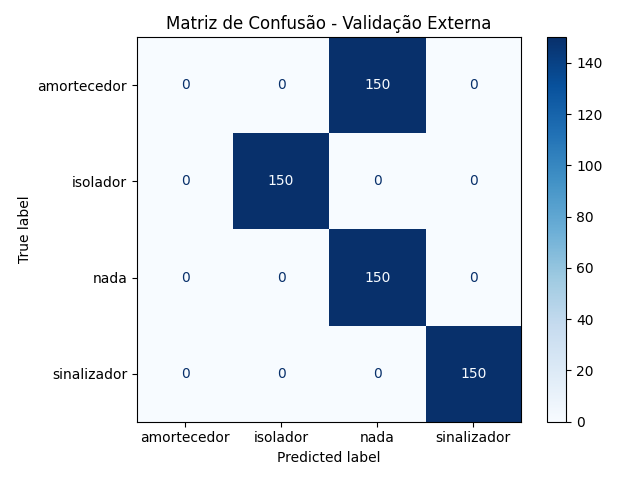
\includegraphics[width=0.7\textwidth]{figuras/Resultados/multi_primeiro_Teste3_nn.png}
\label{fig:mc_featimg_nn_robo1_t3}
\fonte{}
\end{figure}

\begin{figure}[H]
\centering
\caption{Matriz de confusão para a Floresta Aleatória com features extraídas das imagens (primeiro robô das topologias secundárias).}
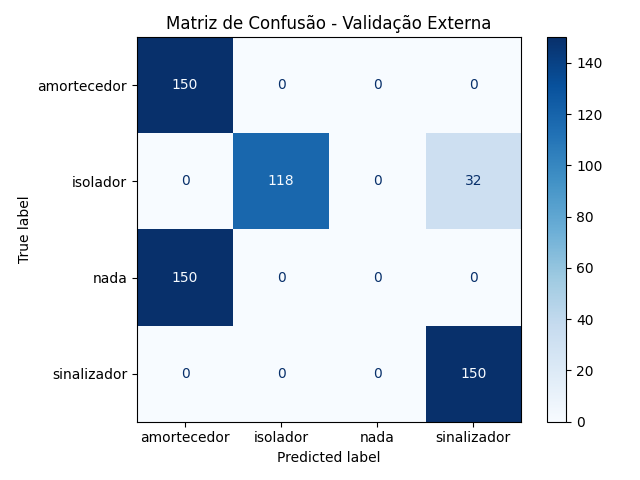
\includegraphics[width=0.7\textwidth]{figuras/Resultados/multi_primeiro_Teste3_rf.png}
\label{fig:mc_featimg_rf_robo1_t3}
\fonte{}
\end{figure}

\subsubsection{Features extraídas do LiDAR}

Esta subseção apresenta os resultados obtidos a partir de atributos derivados dos dados de distância do sensor \textit{LiDAR}, capturadas pelo primeiro robô das topologias secundárias em ambiente simulado com o modelo treinado pelos dados do robô principal. As imagens foram processadas para extrair informações relevantes (\textit{features}) que pudessem melhorar a capacidade dos modelos de aprendizado de máquina na identificação das classes de objetos.

\begin{table}[H]
\caption{Desempenho dos modelos com features extraídas do LiDAR (primeiro robô das topologias secundárias).}
\centering
\begin{tabular}{ccccc}
\hline
\textbf{Modelo} & \textbf{Época Final} & \textbf{Perda Final} & \textbf{Acurácia (\%)} & \textbf{Tempo de Validação (s)}  \\
\hline
kNN      & - & - & 79.83 & 0.012294 \\
Árvore   & - & - & 79.00 & 0.000156 \\
Naive    & - & - & 63.00 & 0.000232 \\
Rede     & 200 & 0.205509 & 69.17 & 0.015490 \\
Floresta & - & - & 80.33 & 0.008353 \\
\hline
\multicolumn{3}{c}{Média} & 74.27 & 0.007305 \\
\hline
\end{tabular}
\fonte{}
\label{tab:modelos_feat_lidar_robo1}
\end{table}

\begin{figure}[H]
\centering
\caption{Matriz de confusão para o k-Vizinhos mais próximos com features extraídas do LiDAR (primeiro robô das topologias secundárias).}
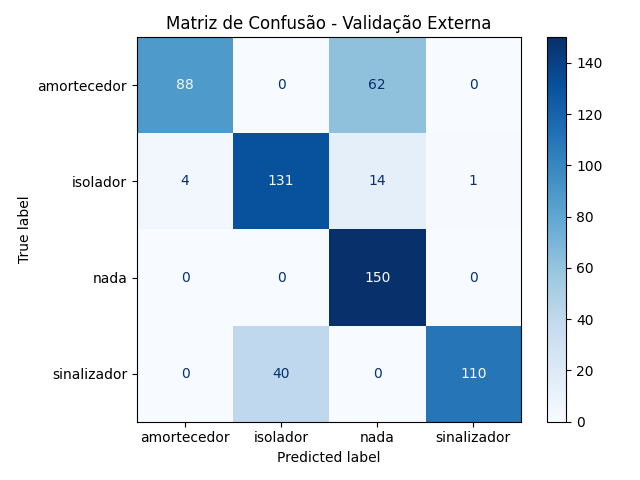
\includegraphics[width=0.7\textwidth]{figuras/Resultados/multi_primeiro_Teste4_knn.png}
\label{fig:mc_featlidar_knn_robo1_t4}
\fonte{}
\end{figure}

\begin{figure}[H]
\centering
\caption{Matriz de confusão para a Árvore de Decisão com features extraídas do LiDAR (primeiro robô das topologias secundárias).}
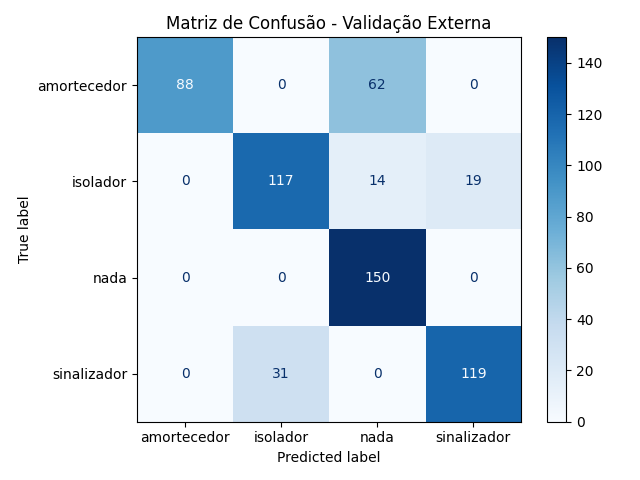
\includegraphics[width=0.7\textwidth]{figuras/Resultados/multi_primeiro_Teste4_tree.png}
\label{fig:mc_featlidar_tree_robo1_t4}
\fonte{}
\end{figure}

\begin{figure}[H]
\centering
\caption{Matriz de confusão para o Naive Bayes com features extraídas do LiDAR (primeiro robô das topologias secundárias).}
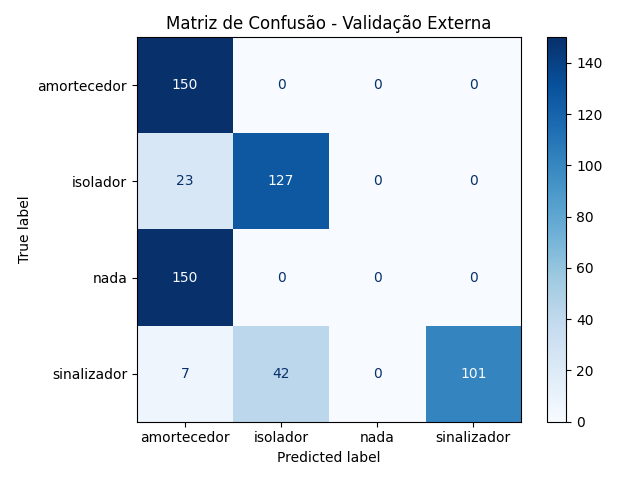
\includegraphics[width=0.7\textwidth]{figuras/Resultados/multi_primeiro_Teste4_naive.png}
\label{fig:mc_featlidar_naive_robo1_t4}
\fonte{}
\end{figure}

\begin{figure}[H]
\centering
\caption{Matriz de confusão para a Rede Neural com features extraídas do LiDAR (primeiro robô das topologias secundárias).}
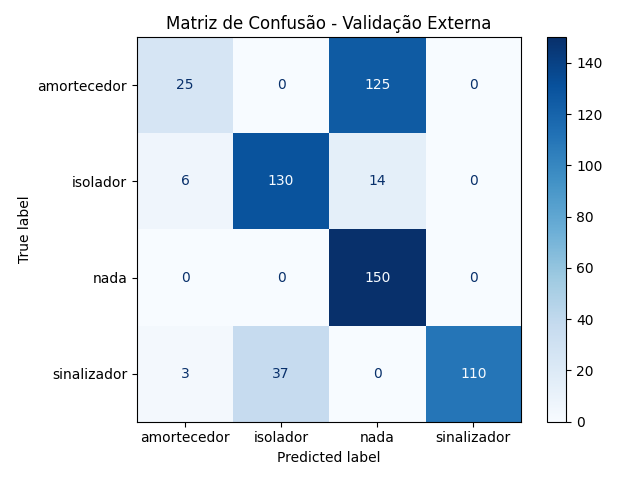
\includegraphics[width=0.7\textwidth]{figuras/Resultados/multi_primeiro_Teste4_nn.png}
\label{fig:mc_featlidar_nn_robo1_t4}
\fonte{}
\end{figure}

\begin{figure}[H]
\centering
\caption{Matriz de confusão para a Floresta Aleatória com features extraídas do LiDAR (primeiro robô das topologias secundárias).}
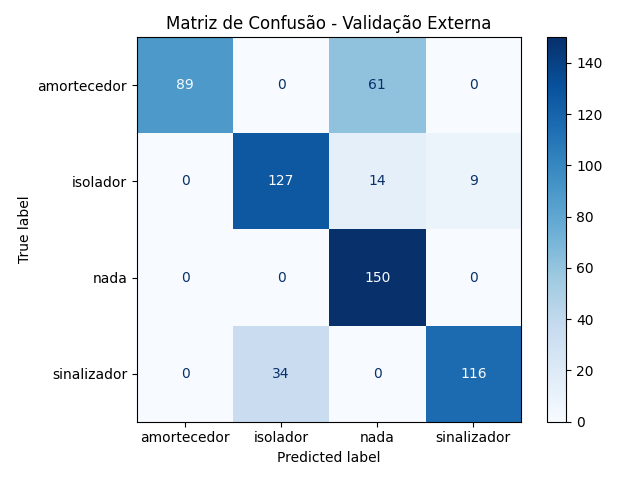
\includegraphics[width=0.7\textwidth]{figuras/Resultados/multi_primeiro_Teste4_rf.png}
\label{fig:mc_featlidar_rf_robo1_t4}
\fonte{}
\end{figure}

\subsubsection{Features combinadas}

Esta subseção apresenta os resultados obtidos a partir da combinação das \textit{features}
extraídas das imagens e dos dados do sensor \textit{LiDAR}, capturadas pelo primeiro robô das topologias secundárias em ambiente simulado com o modelo treinado pelos dados do robô principal.

\begin{table}[H]
\caption{Desempenho dos modelos com features combinadas (primeiro robô das topologias secundárias).}
\centering
\begin{tabular}{ccccc}
\hline
\textbf{Modelo} & \textbf{Época Final} & \textbf{Perda Final} & \textbf{Acurácia (\%)} & \textbf{Tempo de Validação (s)}  \\
\hline
kNN      & - & - & 70.33 & 0.011850 \\
Árvore   & - & - & 69.67 & 0.000151 \\
Naive    & - & - & 69.83 & 0.000245 \\
Rede     & 61 & 0.000034 & 100.00 & 0.016043 \\
Floresta & - & - & 70.33 & 0.007828 \\
\hline
\multicolumn{3}{c}{Média} & 76.03 & 0.007223 \\
\hline
\end{tabular}
\fonte{}
\label{tab:modelos_feat_combinadas_robo1}
\end{table}

\begin{figure}[H]
\centering
\caption{Matriz de confusão para o k-Vizinhos mais próximos com features combinadas (primeiro robô das topologias secundárias).}
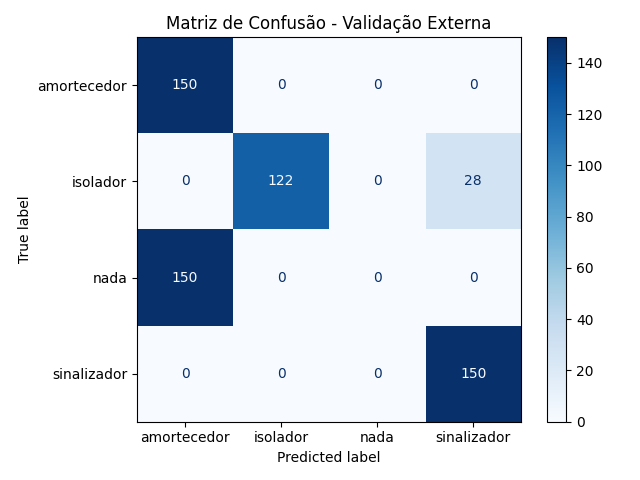
\includegraphics[width=0.7\textwidth]{figuras/Resultados/multi_primeiro_Teste5_knn.png}
\label{fig:mc_featcomb_knn_robo1_t5}
\fonte{}
\end{figure}

\begin{figure}[H]
\centering
\caption{Matriz de confusão para a Árvore de Decisão com features combinadas (primeiro robô das topologias secundárias).}
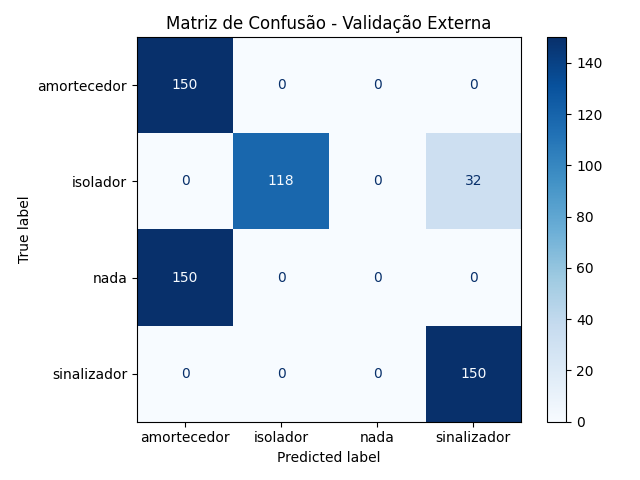
\includegraphics[width=0.7\textwidth]{figuras/Resultados/multi_primeiro_Teste5_tree.png}
\label{fig:mc_featcomb_tree_robo1_t5}
\fonte{}
\end{figure}

\begin{figure}[H]
\centering
\caption{Matriz de confusão para o Naive Bayes com features combinadas (primeiro robô das topologias secundárias).}
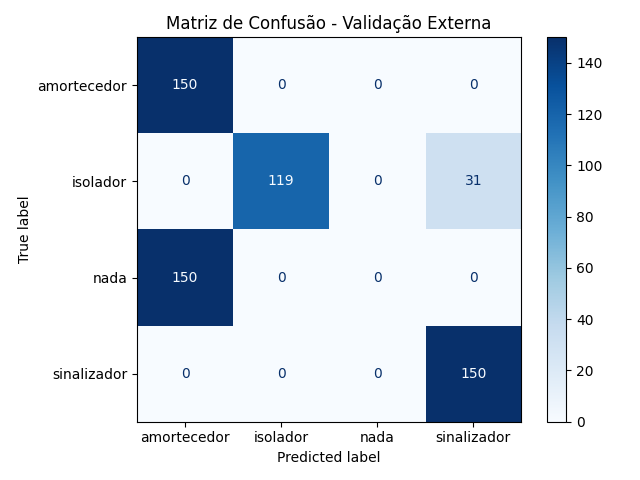
\includegraphics[width=0.7\textwidth]{figuras/Resultados/multi_primeiro_Teste5_naive.png}
\label{fig:mc_featcomb_naive_robo1_t5}
\fonte{}
\end{figure}

\begin{figure}[H]
\centering
\caption{Matriz de confusão para a Floresta Aleatória com features combinadas (primeiro robô das topologias secundárias).}
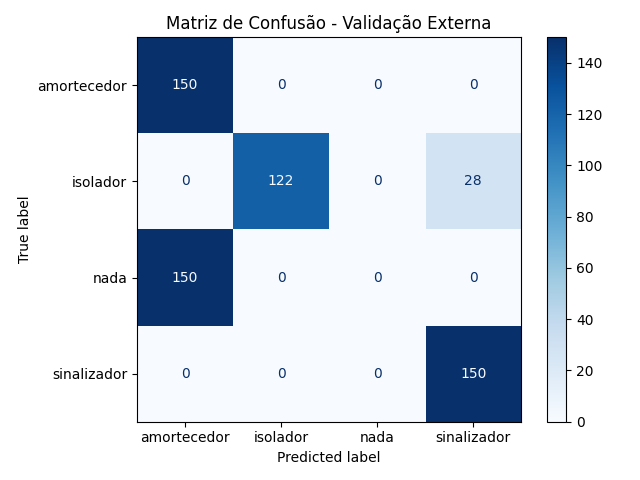
\includegraphics[width=0.7\textwidth]{figuras/Resultados/multi_primeiro_Teste5_rf.png}
\label{fig:mc_featcomb_rf_robo1_t5}
\fonte{}
\end{figure}

\subsection{Dados do segundo robô}

Nesta subseção são apresentados os resultados obtidos a partir dos dados simulados gerados pela segunda topologia secundária em conjunto com os dados do robô principal usados para treinamento. Os resultados serão resumidos nas médias obtidas.

\subsubsection{Imagens brutas}

Esta subseção apresenta os resultados obtidos com as imagens de profundidade brutas
capturadas pelo segundo robô das topologias secundárias em ambiente simulado com o modelo treinado pelos dados do robô principal.


\begin{table}[H]
\caption{Desempenho da SqueezeNet com imagens brutas (robô 1 das topologias secundárias).}
\centering
\begin{tabular}{ccccc}
\hline
\textbf{Época Final} & \textbf{Perda Final} & \textbf{Acurácia (\%)} & \textbf{Tempo de Validação (s)}  \\
\hline
5 & 0.000236 & 97.67 & 3.340613 \\
\hline
\end{tabular}
\fonte{}
\label{tab:resultados_nn2_topo_secundarias}
\end{table}

\subsubsection{Dados brutos do LiDAR}

Esta subseção apresenta os resultados obtidos com os dados brutos do LiDAR capturadas pelo segundo robô das topologias secundárias em ambiente simulado com o modelo treinado pelos dados do robô principal.

\begin{table}[H]
\caption{Desempenho dos modelos com dados brutos do LiDAR (segundo robô das topologias secundárias).}
\centering
\begin{tabular}{ccccc}
\hline
\textbf{Modelo} & \textbf{Época Final} & \textbf{Perda Final} & \textbf{Acurácia (\%)} & \textbf{Tempo de Validação (s)}  \\
\hline
kNN      & - & - & 78.00 & 0.019251 \\
Árvore   & - & - & 52.67 & 0.000230 \\
Naive    & - & - & 36.50 & 0.000785 \\
Rede     & 200 & 0.032724 & 76.33 & 0.015708 \\
Floresta & - & - & 77.50 & 0.007995 \\
\hline
\multicolumn{3}{c}{Média} & 64.20 & 0.043447 \\
\hline
\end{tabular}
\fonte{}
\label{tab:modelos_lidar_bruto_robo2}
\end{table}

% Figuras para a subseção "Dados brutos do LiDAR" (Segundo Robô)
% Contexto: segundo robô das topologias secundárias. Nomes dos arquivos indicam Teste2.

\begin{figure}[H]
\centering
\caption{Matriz de confusão para o k-Vizinhos mais próximos com dados brutos do LiDAR (segundo robô das topologias secundárias).}
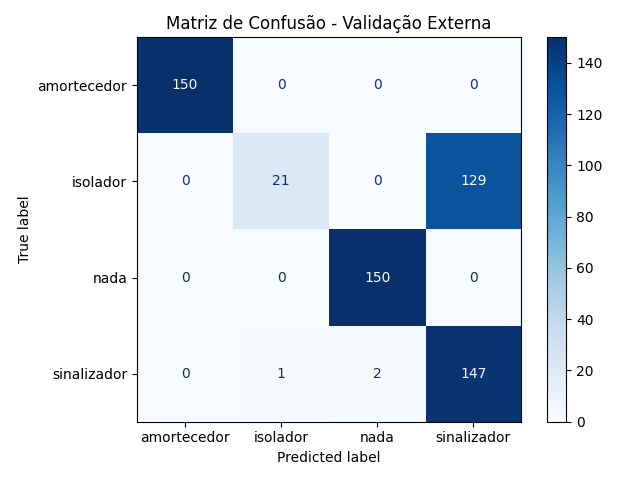
\includegraphics[width=0.7\textwidth]{figuras/Resultados/multi_segundo_Teste2_knn.png}
\label{fig:mc_lidar_knn_robo2_t2}
\fonte{}
\end{figure}

\begin{figure}[H]
\centering
\caption{Matriz de confusão para a Árvore de Decisão com dados brutos do LiDAR (segundo robô das topologias secundárias).}
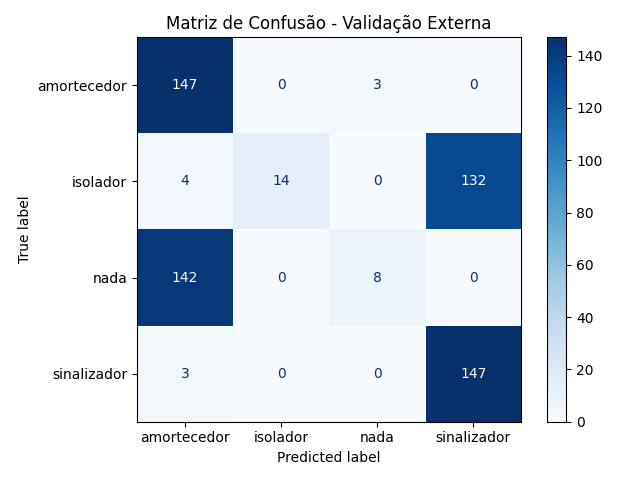
\includegraphics[width=0.7\textwidth]{figuras/Resultados/multi_segundo_Teste2_tree.png}
\label{fig:mc_lidar_tree_robo2_t2}
\fonte{}
\end{figure}

\begin{figure}[H]
\centering
\caption{Matriz de confusão para o Naive Bayes com dados brutos do LiDAR (segundo robô das topologias secundárias).}
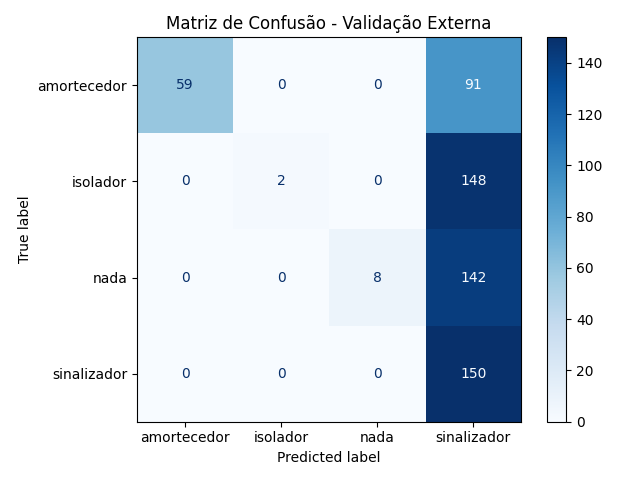
\includegraphics[width=0.7\textwidth]{figuras/Resultados/multi_segundo_Teste2_naive.png}
\label{fig:mc_lidar_naive_robo2_t2}
\fonte{}
\end{figure}

\begin{figure}[H]
\centering
\caption{Matriz de confusão para a Rede Neural com dados brutos do LiDAR (segundo robô das topologias secundárias).}
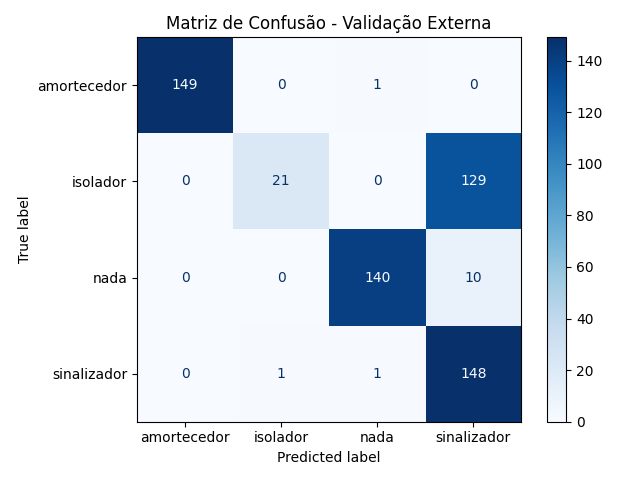
\includegraphics[width=0.7\textwidth]{figuras/Resultados/multi_segundo_Teste2_nn.png}
\label{fig:mc_lidar_nn_robo2_t2}
\fonte{}
\end{figure}

\begin{figure}[H]
\centering
\caption{Matriz de confusão para a Floresta Aleatória com dados brutos do LiDAR (segundo robô das topologias secundárias).}
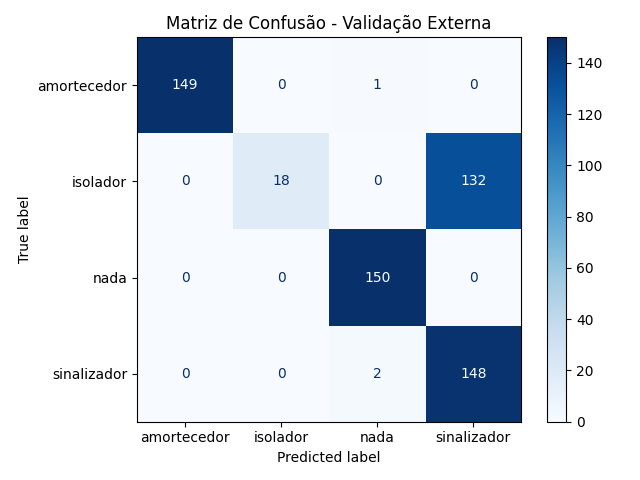
\includegraphics[width=0.7\textwidth]{figuras/Resultados/multi_segundo_Teste2_rf.png}
\label{fig:mc_lidar_rf_robo2_t2}
\fonte{}
\end{figure}

\subsubsection{Features extraídas das imagens}

Esta subseção apresenta os resultados obtidos a partir de atributos derivados das imagens capturadas pelo segundo robô das topologias secundárias em ambiente simulado com o modelo treinado pelos dados do robô principal. As imagens foram processadas para extrair informações relevantes (\textit{features}) que pudessem melhorar a capacidade dos modelos de aprendizado de máquina na identificação das classes de objetos.

\begin{table}[H]
\caption{Desempenho dos modelos com features extraídas das imagens (segundo robô das topologias secundárias).}
\centering
\begin{tabular}{ccccc}
\hline
\textbf{Modelo} & \textbf{Época Final} & \textbf{Perda Final} & \textbf{Acurácia (\%)} & \textbf{Tempo de Validação (s)}  \\
\hline
kNN      & - & - & 86.67 & 0.011986 \\
Árvore   & - & - & 61.17 & 0.000149 \\
Naive    & - & - & 47.33 & 0.000305 \\
Rede     & 60 & 0.000764 & 88.50 & 0.017994 \\
Floresta & - & - & 64.83 & 0.008024 \\
\hline
\multicolumn{3}{c}{Média} & 69.70 & 0.007692 \\
\hline
\end{tabular}
\fonte{}
\label{tab:modelos_featimg_robo2}
\end{table}

% Figuras para a subseção "Features extraídas das imagens" (Segundo Robô)
% Contexto: segundo robô das topologias secundárias. Nomes dos arquivos indicam Teste3.

\begin{figure}[H]
\centering
\caption{Matriz de confusão para o k-Vizinhos mais próximos com features extraídas das imagens (segundo robô das topologias secundárias).}
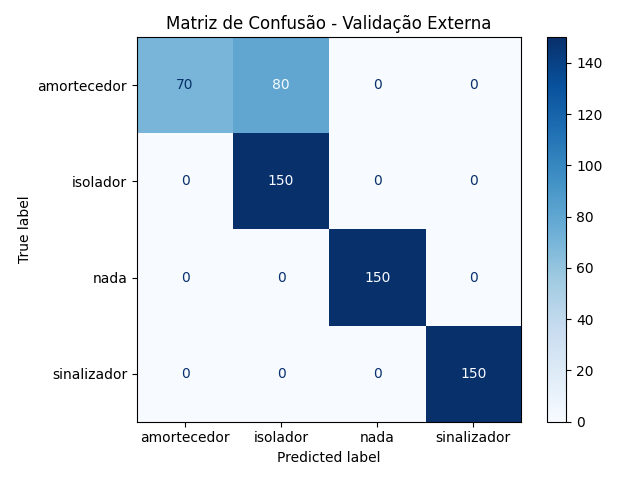
\includegraphics[width=0.7\textwidth]{figuras/Resultados/multi_segundo_Teste3_knn.png}
\label{fig:mc_featimg_knn_robo2_t3}
\fonte{}
\end{figure}

\begin{figure}[H]
\centering
\caption{Matriz de confusão para a Árvore de Decisão com features extraídas das imagens (segundo robô das topologias secundárias).}
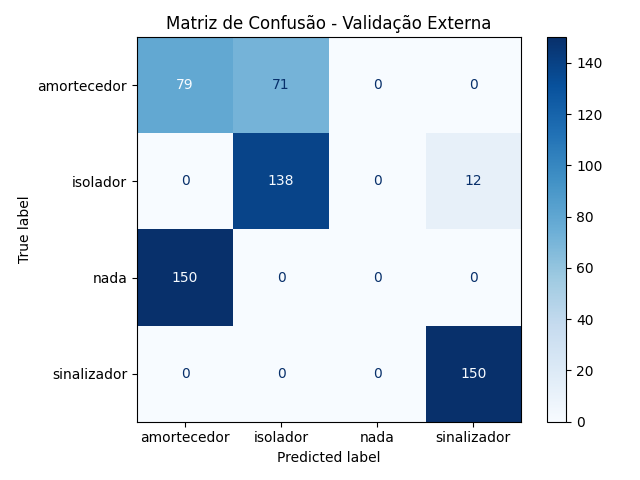
\includegraphics[width=0.7\textwidth]{figuras/Resultados/multi_segundo_Teste3_tree.png}
\label{fig:mc_featimg_tree_robo2_t3}
\fonte{}
\end{figure}

\begin{figure}[H]
\centering
\caption{Matriz de confusão para o Naive Bayes com features extraídas das imagens (segundo robô das topologias secundárias).}
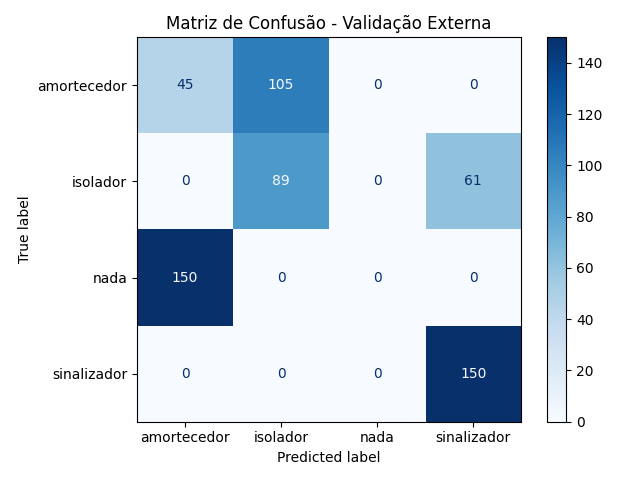
\includegraphics[width=0.7\textwidth]{figuras/Resultados/multi_segundo_Teste3_naive.png}
\label{fig:mc_featimg_naive_robo2_t3}
\fonte{}
\end{figure}

\begin{figure}[H]
\centering
\caption{Matriz de confusão para a Rede Neural com features extraídas das imagens (segundo robô das topologias secundárias).}
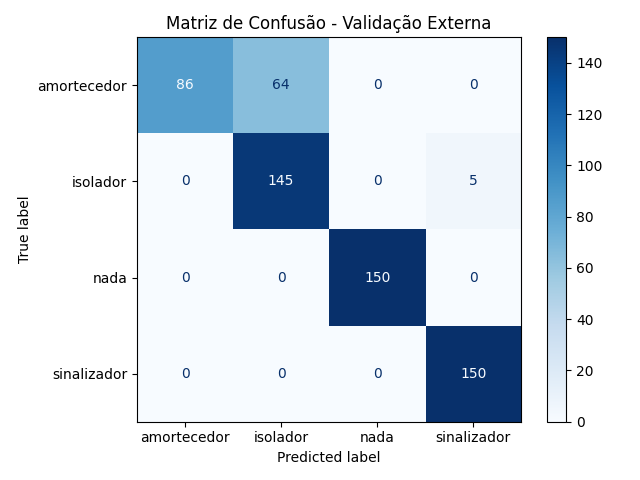
\includegraphics[width=0.7\textwidth]{figuras/Resultados/multi_segundo_Teste3_nn.png}
\label{fig:mc_featimg_nn_robo2_t3}
\fonte{}
\end{figure}

\begin{figure}[H]
\centering
\caption{Matriz de confusão para a Floresta Aleatória com features extraídas das imagens (segundo robô das topologias secundárias).}
\includegraphics[width=0.7\textwidth]{figuras/Resultados/multi_segundo_Teste3_rf.png}
\label{fig:mc_featimg_rf_robo2_t3}
\fonte{}
\end{figure}

\subsubsection{Features extraídas do LiDAR}

Esta subseção apresenta os resultados obtidos a partir de atributos derivados dos dados de distância do sensor \textit{LiDAR}, capturadas pelo segundo robô das topologias secundárias em ambiente simulado com o modelo treinado pelos dados do robô principal. As imagens foram processadas para extrair informações relevantes (\textit{features}) que pudessem melhorar a capacidade dos modelos de aprendizado de máquina na identificação das classes de objetos.

\begin{table}[H]
\caption{Desempenho dos modelos com features extraídas do LiDAR (segundo robô das topologias secundárias).}
\centering
\begin{tabular}{ccccc}
\hline
\textbf{Modelo} & \textbf{Época Final} & \textbf{Perda Final} & \textbf{Acurácia (\%)} & \textbf{Tempo de Validação (s)}  \\
\hline
kNN      & - & - & 74.33 & 0.013072 \\
Árvore   & - & - & 74.50 & 0.000177 \\
Naive    & - & - & 71.67 & 0.000255 \\
Rede     & 200 & 0.283318 & 93.50 & 0.015820 \\
Floresta & - & - & 80.67 & 0.007872 \\
\hline
\multicolumn{3}{c}{Média} & 78.93 & 0.007439 \\
\hline
\end{tabular}
\fonte{}
\label{tab:modelos_featlidar_robo2}
\end{table}

\begin{figure}[H]
\centering
\caption{Matriz de confusão para o k-Vizinhos mais próximos com features extraídas do LiDAR (segundo robô das topologias secundárias).}
\includegraphics[width=0.7\textwidth]{figuras/Resultados/multi_segundo_Teste4_knn.png}
\label{fig:mc_featlidar_knn_robo2_t4}
\fonte{}
\end{figure}

\begin{figure}[H]
\centering
\caption{Matriz de confusão para a Árvore de Decisão com features extraídas do LiDAR (segundo robô das topologias secundárias).}
\includegraphics[width=0.7\textwidth]{figuras/Resultados/multi_segundo_Teste4_tree.png}
\label{fig:mc_featlidar_tree_robo2_t4}
\fonte{}
\end{figure}

\begin{figure}[H]
\centering
\caption{Matriz de confusão para o Naive Bayes com features extraídas do LiDAR (segundo robô das topologias secundárias).}
\includegraphics[width=0.7\textwidth]{figuras/Resultados/multi_segundo_Teste4_naive.png}
\label{fig:mc_featlidar_naive_robo2_t4}
\fonte{}
\end{figure}

\begin{figure}[H]
\centering
\caption{Matriz de confusão para a Rede Neural com features extraídas do LiDAR (segundo robô das topologias secundárias).}
\includegraphics[width=0.7\textwidth]{figuras/Resultados/multi_segundo_Teste4_nn.png}
\label{fig:mc_featlidar_nn_robo2_t4}
\fonte{}
\end{figure}

\begin{figure}[H]
\centering
\caption{Matriz de confusão para a Floresta Aleatória com features extraídas do LiDAR (segundo robô das topologias secundárias).}
\includegraphics[width=0.7\textwidth]{figuras/Resultados/multi_segundo_Teste4_rf.png}
\label{fig:mc_featlidar_rf_robo2_t4}
\fonte{}
\end{figure}

\subsubsection{Features combinadas}

Esta subseção apresenta os resultados obtidos a partir da combinação das \textit{features}
extraídas das imagens e dos dados do sensor \textit{LiDAR}, capturadas pelo segundo robô das topologias secundárias em ambiente simulado com o modelo treinado pelos dados do robô principal.

\begin{table}[H]
\caption{Desempenho dos modelos com features combinadas (segundo robô das topologias secundárias).}
\centering
\begin{tabular}{ccccc}
\hline
\textbf{Modelo} & \textbf{Época Final} & \textbf{Perda Final} & \textbf{Acurácia (\%)} & \textbf{Tempo de Validação (s)}  \\
\hline
kNN      & - & - & 86.67 & 0.011865 \\
Árvore   & - & - & 84.67 & 0.000149 \\
Naive    & - & - & 49.50 & 0.000358 \\
Rede     & 71 & 0.000686 & 88.50 & 0.015628 \\
Floresta & - & - & 64.83 & 0.006904 \\
\hline
\multicolumn{3}{c}{Média} & 74.83 & 0.006981 \\
\hline
\end{tabular}
\fonte{}
\label{tab:modelos_featcomb_robo2}
\end{table}

\begin{figure}[H]
\centering
\caption{Matriz de confusão para o k-Vizinhos mais próximos com features combinadas (segundo robô das topologias secundárias).}
\includegraphics[width=0.7\textwidth]{figuras/Resultados/multi_segundo_Teste5_knn.png}
\label{fig:mc_featcomb_knn_robo2_t5}
\fonte{}
\end{figure}

\begin{figure}[H]
\centering
\caption{Matriz de confusão para a Árvore de Decisão com features combinadas (segundo robô das topologias secundárias).}
\includegraphics[width=0.7\textwidth]{figuras/Resultados/multi_segundo_Teste5_tree.png}
\label{fig:mc_featcomb_tree_robo2_t5}
\fonte{}
\end{figure}

\begin{figure}[H]
\centering
\caption{Matriz de confusão para o Naive Bayes com features combinadas (segundo robô das topologias secundárias).}
\includegraphics[width=0.7\textwidth]{figuras/Resultados/multi_segundo_Teste5_naive.png}
\label{fig:mc_featcomb_naive_robo2_t5}
\fonte{}
\end{figure}

\begin{figure}[H]
\centering
\caption{Matriz de confusão para a Rede Neural com features combinadas (segundo robô das topologias secundárias).}
\includegraphics[width=0.7\textwidth]{figuras/Resultados/multi_segundo_Teste5_nn.png}
\label{fig:mc_featcomb_nn_robo2_t5}
\fonte{}
\end{figure}

\begin{figure}[H]
\centering
\caption{Matriz de confusão para a Floresta Aleatória com features combinadas (segundo robô das topologias secundárias).}
\includegraphics[width=0.7\textwidth]{figuras/Resultados/multi_segundo_Teste5_rf.png}
\label{fig:mc_featcomb_rf_robo2_t5}
\fonte{}
\end{figure}

%-----------------------------------------------------------%%% Apêndice - Comente para remover este item
   %%%%% APÊNDICE B
%%
%% Texto ou documento elaborado pelo autor, a fim de complementar sua argumentação, sem prejuízo da unidade nuclear do trabalho.

%% Título e rótulo de apêndice (rótulos não devem conter caracteres especiais, acentuados ou cedilha)
\chapter{Roteiro da entrevista}\label{cap:apendiceb}

\begin{table}[htb]%% Ambiente table
\caption{Orçamento dos materiais n.\textsuperscript{o} 1.}%% Legenda
\label{tab:tab3}%% Rótulo
\begin{tabularx}{\textwidth}{@{\extracolsep{\fill}}lrrr}%% Ambiente tabularx
\toprule
Material              & \multicolumn{1}{c}{Valor (R\$)} & \multicolumn{1}{c}{Quantidade}  & \multicolumn{1}{c}{Total (R\$)} \\ \midrule
Bomba centrífuga      & 2500,00                         & 01                              & 2500,00                         \\
Compressor rotativo   & 3000,00                         & 01                              & 3000,00                         \\
Manômetro diferencial & 450,00                          & 02                              & 900,00                          \\
Termopar              & 370,00                          & 02                              & 740,00                          \\
Válvula de esfera     & 43,00                           & 02                              & 86,00                           \\
Tubulação de PVC      & 10,00                           & 05                              & 50,00                           \\
Conexão de PVC        & 5,00                            & 10                              & 50,00                           \\ \midrule
                      &                                 & \multicolumn{1}{r}{Total (R\$)} & 7326,00                         \\ \bottomrule
\end{tabularx}
\fonte{}%% Fonte
\end{table}

\begin{table}[htb]%% Ambiente table
\caption{Orçamento dos materiais n.\textsuperscript{o} 2.}%% Legenda
\label{tab:tab4}%% Rótulo
\begin{tabularx}{\textwidth}{@{\extracolsep{\fill}}lrrr}%% Ambiente tabularx
\toprule
Material              & \multicolumn{1}{c}{Valor (R\$)} & \multicolumn{1}{c}{Quantidade}  & \multicolumn{1}{c}{Total (R\$)} \\ \midrule
Bomba centrífuga      & 2700,00                         & 01                              & 2700,00                         \\
Compressor rotativo   & 2950,00                         & 01                              & 2950,00                         \\
Manômetro diferencial & 515,00                          & 02                              & 1030,00                         \\
Termopar              & 350,00                          & 02                              & 700,00                          \\
Válvula de esfera     & 40,00                           & 02                              & 80,00                           \\
Tubulação de PVC      & 8,00                            & 05                              & 40,00                           \\
Conexão de PVC        & 6,00                            & 10                              & 60,00                           \\ \midrule
                      &                                 & \multicolumn{1}{r}{Total (R\$)} & 7560,00                         \\ \bottomrule
\end{tabularx}
\fonte{}%% Fonte
\end{table}

\begin{table}[htb]%% Ambiente table
\caption{Orçamento dos materiais n.\textsuperscript{o} 3.}%% Legenda
\label{tab:tab5}%% Rótulo
\begin{tabularx}{\textwidth}{@{\extracolsep{\fill}}lrrr}%% Ambiente tabularx
\toprule
Material              & \multicolumn{1}{c}{Valor (R\$)} & \multicolumn{1}{c}{Quantidade}  & \multicolumn{1}{c}{Total (R\$)} \\ \midrule
Bomba centrífuga      & 2600,00                         & 01                              & 2600,00                         \\
Compressor rotativo   & 3100,00                         & 01                              & 3100,00                         \\
Manômetro diferencial & 500,00                          & 02                              & 1000,00                         \\
Termopar              & 400,00                          & 02                              & 800,00                          \\
Válvula de esfera     & 45,00                           & 02                              & 90,00                           \\
Tubulação de PVC      & 12,00                           & 05                              & 60,00                           \\
Conexão de PVC        & 5,00                            & 10                              & 50,00                           \\ \midrule
                      &                                 & \multicolumn{1}{r}{Total (R\$)} & 7700,00                         \\ \bottomrule
\end{tabularx}
\fonte{}%% Fonte
\end{table}
%% Apêndice - Comente para remover este item
 \end{arquivosdeapendices}%% Não comente esta linha


% \begin{apendicesenv}%% Ambiente apendicesenv

% \partapendices
% \chapter{Ola}

% \lipsum[55-56]

% \end{apendicesenv}

%% Arquivos de anexos
\begin{arquivosdeanexos}%% Os arquivos de anexos devem se incluídos neste ambiente - Não comente esta linha
  %\partanexos%% Página de início dos anexos - adiciona uma página com o título Anexos

  %%%%% ANEXO A
%%
%% Texto ou documento não elaborado pelo autor, que serve de fundamentação, comprovação e ilustração.

%% Título e rótulo de anexo (rótulos não devem conter caracteres especiais, acentuados ou cedilha)
\anexos
\chapter{Lei N\texorpdfstring{.\textsuperscript{o}}{o.} 9.610, de 19 de Fevereiro de 1998}\label{cap:anexoa}

\centerline{\includegraphics[width=\textwidth]{./PosTexto/Ilustracoes/lei-n9610-p1}}%% Imagem (Dimensões e localização)

\centerline{\includegraphics[width=\textwidth]{./PosTexto/Ilustracoes/lei-n9610-p2}}%% Imagem (Dimensões e localização)
%% Anexo - Comente para remover este item
  %%%%% ANEXO B
%%
%% Texto ou documento não elaborado pelo autor, que serve de fundamentação, comprovação e ilustração.

%% Título e rótulo de anexo (rótulos não devem conter caracteres especiais, acentuados ou cedilha)
\chapter{Normas para elaboração de trabalhos acadêmicos}\label{cap:anexob}

As normas da \gls{utfpr} podem ser acessadas em: \url{http://portal.utfpr.edu.br/biblioteca/trabalhos-academicos/discentes/orientacao-para-trabalhos-academicos}. Ver Figura \ref{fig:capadolivro}.

\begin{figure}[htb]%% Ambiente figure
\captionsetup{width=0.9\textwidth}%% Largura da legenda
\caption{Sítio: Normas para Elaboração de Trabalhos Acadêmicos.}%% Legenda
\label{fig:capadolivro}%% Rótulo
\includegraphics[width=0.9\textwidth]{normas}%% Dimensões e localização
\fonte{\cite{UTFPR2008}}%% Fonte
\end{figure}

%% Anexo - Comente para remover este item
\end{arquivosdeanexos}%% Não comente esta linha

%% Índice - Adiciona um índice remissivo.
%\incluirindice%% Comente para remover este item

%% Fim do documento
\end{document}%% Não comente esta linha
